\documentclass[11pt]{article}
\usepackage{amsmath}
\usepackage{amssymb}
\usepackage{graphicx}
\usepackage{hyperref}
\usepackage{geometry}
\usepackage{booktabs}
\usepackage{xcolor}
\usepackage{float}

\pdfminorversion=4
\pdfobjcompresslevel=0

\setlength{\parindent}{0pt}


\geometry{a4paper, margin=1in}
\title{BUSFIN 8200 - Problem Set 1}
\author{Maeve Nguyen}
\date{\today}

\begin{document}
\maketitle
\section*{Question 1}
\subsection*{1 (a)}

Starting from $R_{e,t+1} = \frac{P_{t+1} + D_{t+1}}{P_t}$ and assuming that $D$ is greater than zero, we take log of both sides and have:
\[
\begin{aligned}
  r_{e,t+1}
  &= \log(P_{t+1} + D_{t+1}) - \log(P_t) \\
  &= \log(P_{t+1})(1+\frac{D_{t+1}}{P_{t+1}}) -  p_t \\
  &= p_{t+1} + \log(1+ \frac{e^{d_{t+1}}}{e^{p_{t+1}}}) - p_t \\
  &= p_{t+1} + \log(1+ e^{d_{t+1} - p_{t+1}}) - p_t \\
  &= p_{t+1} + \log(1+ e^{dp_{t+1}}) - p_t \\
  &= p_{t+1} - p_t + f(dp_{t+1})
\end{aligned}
\]

where $f(dp_{t+1})$ is a log function of the log dividend-price ratio. Applying a first-order Taylor expansion around $\overline{dp}$ to $f(dp_{t+1})$, we have Equation (1):

\[
\begin{aligned}
    r_{e,t+1}
    \approx p_{t+1} - p_t + f(\overline{dp})+f'(\overline{dp})(dp_{t+1} - \overline{dp}) 
\end{aligned}
\]

We define $\kappa = \frac{1}{1+e^{\overline{dp}}}$. Consequently, we have the following: 
\[
\begin{aligned}
     f'(\overline{dp}) = \frac{e^{\overline{dp}}}{1+e^{\overline{dp}}} &= 1 - \kappa \\
    e^{\overline{dp}} &= \frac{1}{\kappa} - 1 \\
    \overline{dp} &= \log(\frac{1}{\kappa} - 1)
\end{aligned}
\]

Plugging in the above results into Equation (1), we have:

\[
\begin{aligned}
    r_{e,t+1} 
    &\approx p_{t+1} - p_t + \log(1+ e^{\overline{dp}}) + (1 - \kappa)dp_{t+1} -  (1 - \kappa)\log(\frac{1}{\kappa} - 1) \\
    &= p_{t+1} - p_t + \log(\frac{1}{\kappa}) -(1- \kappa)p_{t+1} + (1 -\kappa)d_{t+1} - (1 - \kappa)\log(\frac{1}{\kappa} - 1) \\
    &= \kappa p_{t+1} - p_t + (1- \kappa) d_{t+1} + \kappa_0 \\
    &= \kappa_0 -\kappa dp_{t+1} + (d_{t+1} - d_t) + (d_t- p_t) \\
    &= \kappa_0 - \kappa dp_{t+1} + \Delta d_{t+1} + dp_t 
\end{aligned}
\]
where $\kappa_0 = \log(\frac{1}{\kappa}) - (1 - \kappa)\log(\frac{1}{\kappa} - 1) = -\log(\kappa) - (1 - \kappa)\log(\frac{1}{\kappa} - 1)$. Rearranging the above equation, we have:
\[
\begin{aligned}
    dp_t = -\kappa_0 + \kappa dp_{t+1} + r_{e,t+1} - \Delta d_{t+1} \\
    \Rightarrow dp_{t+1} = -\kappa_0 + \kappa dp_{t+2} + r_{e,t+2} - \Delta d_{t+2} \\
    \Rightarrow dp_{t+2} = -\kappa_0 + \kappa dp_{t+3} + r_{e,t+3} - \Delta d_{t+3} 
\end{aligned}
\]

Keeping substituting these equations into the first one and generalizing the pattern H times, we have:


\begin{align}
    dp_t 
    &= -\kappa_0 \underbrace{(1+\kappa + \kappa^2)}_{\displaystyle \sum_{h=1}^{H} \kappa^{h-1}} + \kappa^3 dp_{t+3} + [r_{e,t+1} + \kappa r_{e,t+2} + \kappa^2 r_{e,t+3}] - [\Delta d_{t+1} + \kappa \Delta d_{t+2} + \kappa^2 \Delta d_{t+3}] \notag \\
    &= -\kappa_0 (\frac{1-\kappa^H}{1-\kappa}) + \kappa^H \cdot dp_{t+H} + \sum_{h=1}^{H} \kappa^{h-1} \cdot r_{e,t+h} - \sum_{h=1}^{H} \kappa^{h-1} \cdot \Delta d_{t+h} \notag \\
    &= \kappa_0 (\frac{\kappa^H-1}{1-\kappa}) + \kappa^H \cdot dp_{t+H} + \sum_{h=1}^{H} \kappa^{h-1} \cdot r_{e,t+h} - \sum_{h=1}^{H} \kappa^{h-1} \cdot \Delta d_{t+h}  \tag*{\color{red}(1.1)}
\end{align}

Given that $\mathbb{E}_t[dp_t] = dp_t$, we take conditional expectation on both sides of Equation {\color{red}(1.1)} and have:

\begin{align}
    dp_t
    &= \kappa_0 (\frac{\kappa^H-1}{1-\kappa}) + \kappa^H \cdot \mathbb{E}_t[dp_{t+H}] + \sum_{h=1}^{H} \kappa^{h-1} \cdot \mathbb{E}_t[r_{e,t+h}] - \sum_{h=1}^{H} \kappa^{h-1} \cdot \mathbb{E}_t[\Delta d_{t+h}]
    \tag*{\color{red}(1.2)}
\end{align}

Since $e^{\overline{dp}}$ is always positive, we have $0 < \kappa < 1$. Therefore, as $H \to \infty$, $\kappa^H \to 0$. In addition, we also need to impose No-Bubble Condition such that $\lim_{H \to \infty} \kappa^H \cdot \mathbb{E}_t[dp_{t+H}] = 0$. Giglio, Maggiori, and Stroebel (2016) indeed shows that there were no systemic deviations in the discounts of extremely long leaseholds to otherwise identical freeholds in the U.K. and Singapore housing markets, thus indicating no rational bubbles. Consequently, letting $H \to \infty$, Equation {\color{red}(1.2)} can be simplified as follows:
\begin{align}
    dp_t
    &= \frac{-\kappa_0}{1-\kappa}+ \sum_{h=1}^{\infty} \kappa^{h-1} \cdot \mathbb{E}_t[r_{e,t+h}] - \sum_{h=1}^{\infty} \kappa^{h-1} \cdot \mathbb{E}_t[\Delta d_{t+h}]
    \tag*{\color{red}(1.3)}
\end{align}

\subsection*{1 (b)}
Using Equation 1.4 from the problem set, I decomposed the variation in the log dividend-price ratio into variations associated with the discounted future returns, discounted future dividend growth and terminal dividend-price ratio. By constructing these regressors at a 12-month increment, I regressed each component on $dp_t$ in univariate OLS models to estimate their respective betas through different horizons as shown below. 
\begin{figure}[H]
    \centering
    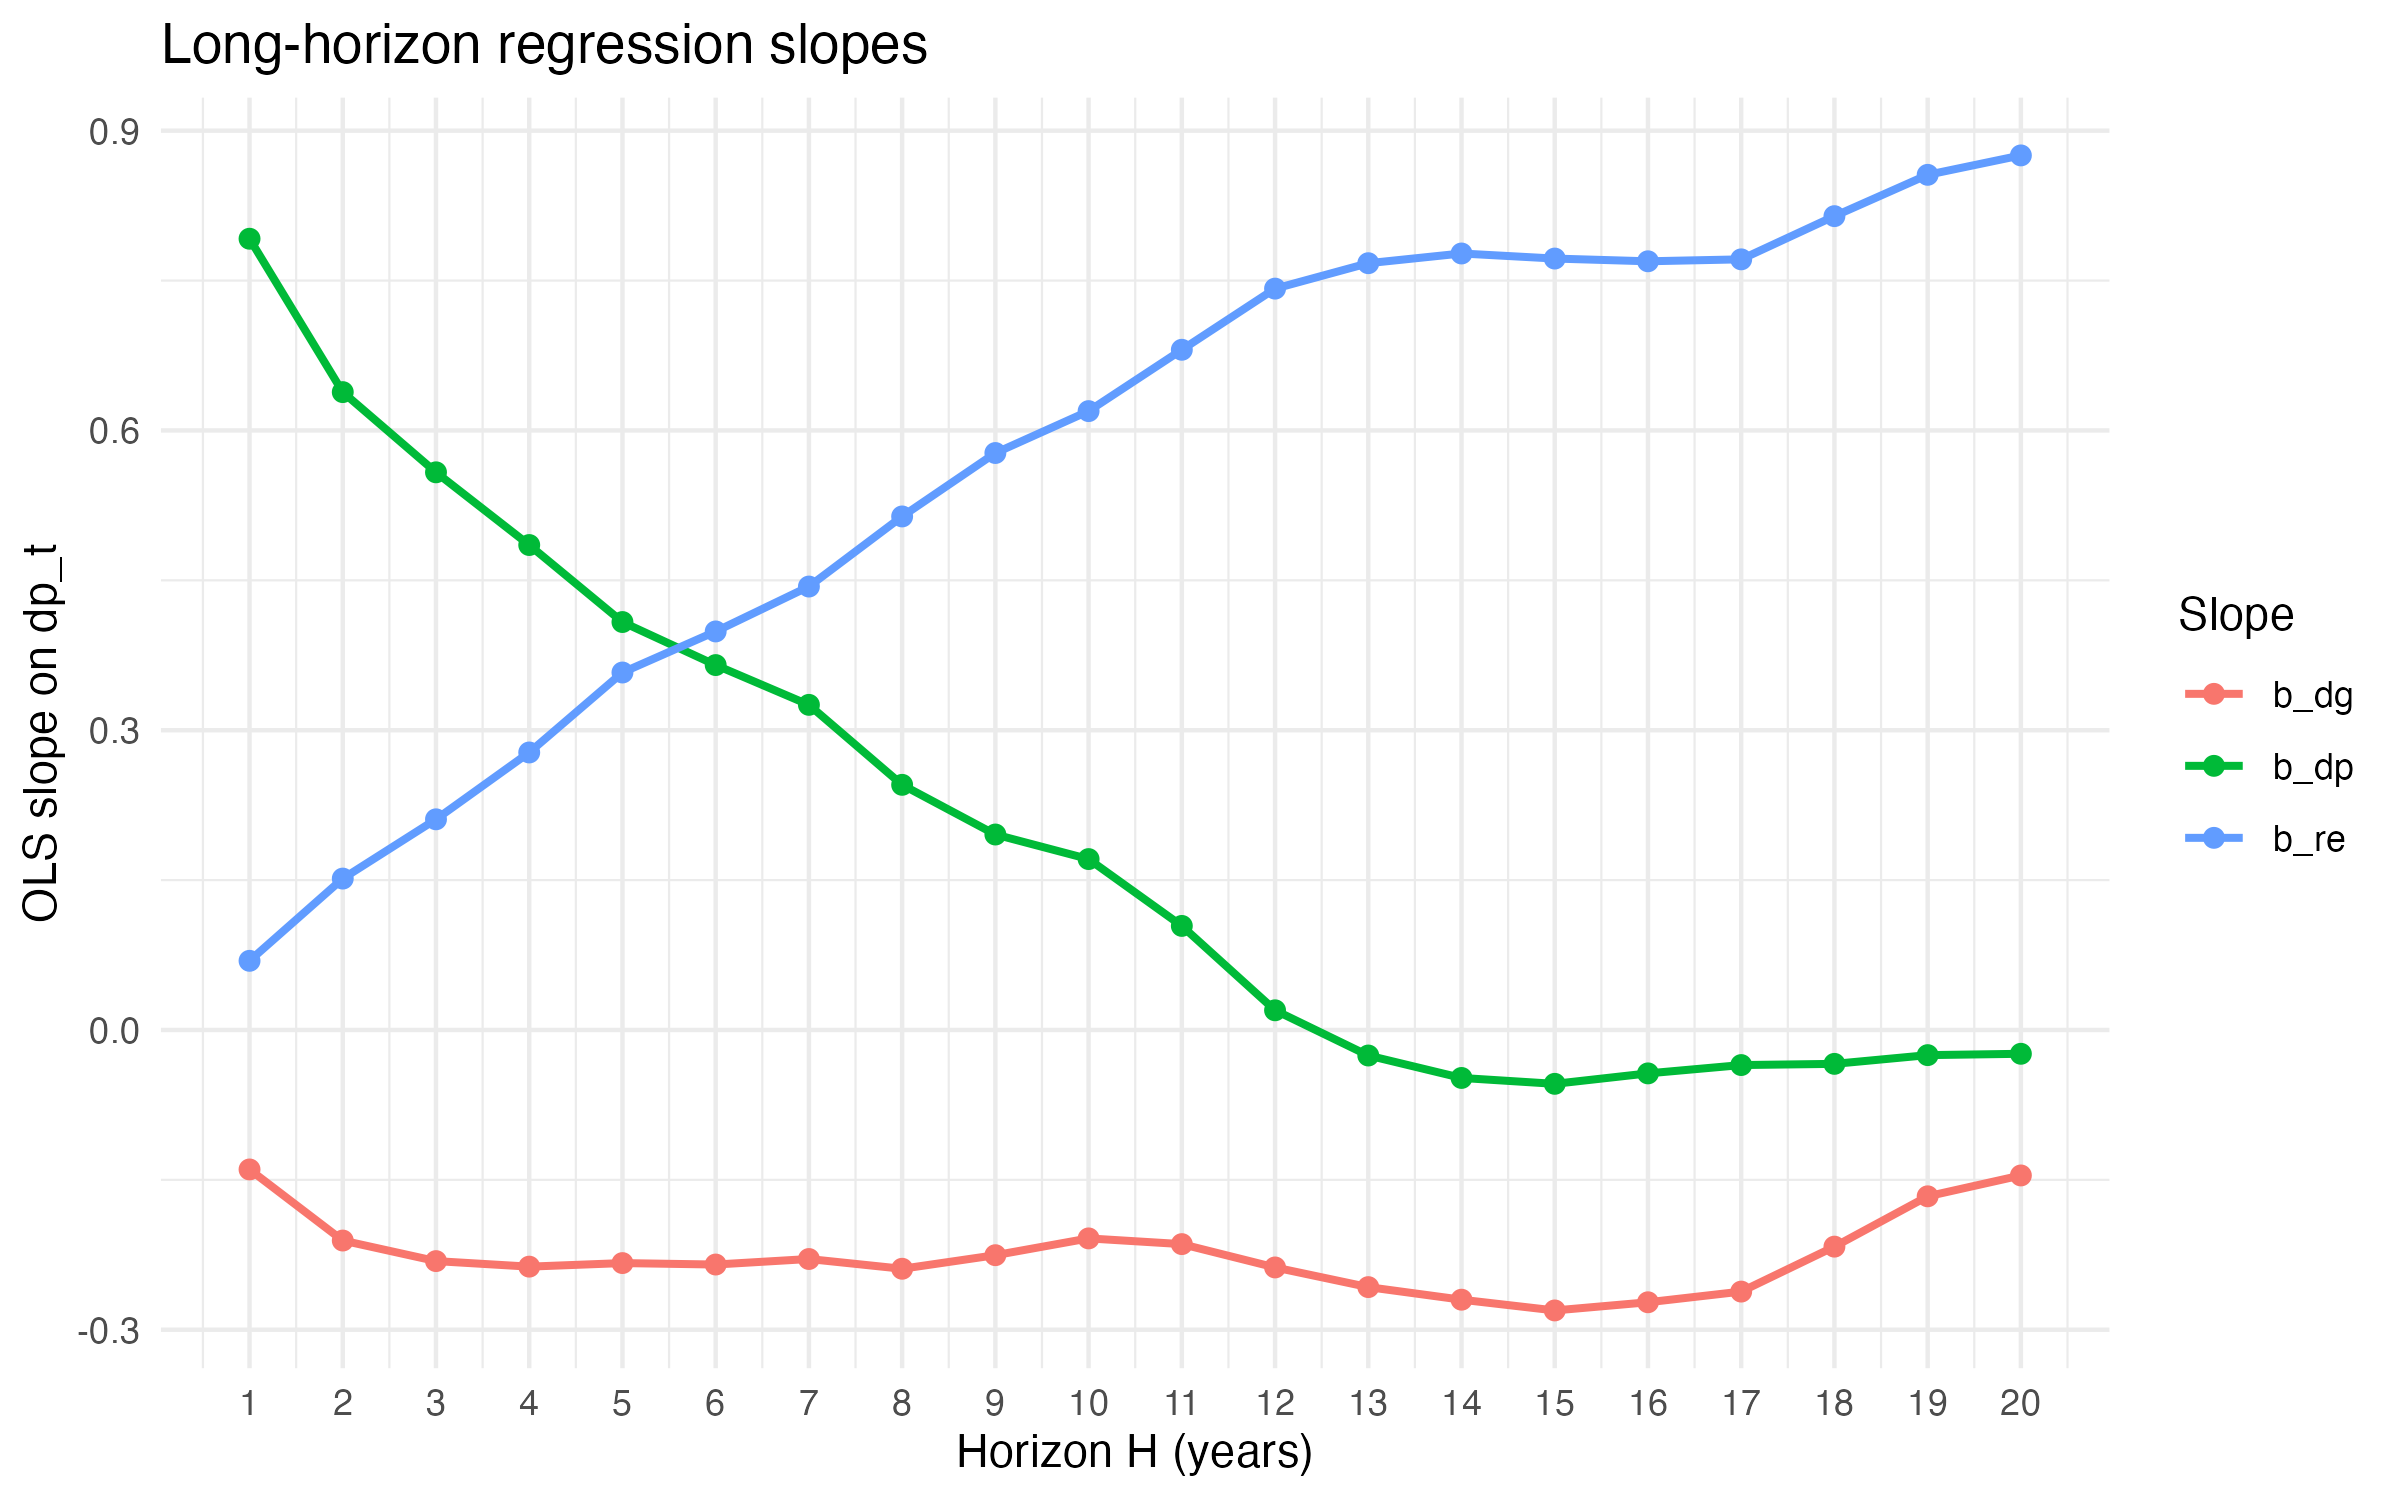
\includegraphics[width=0.6\textwidth]{figures/1b_figure.png}
    \label{fig:q1}
\end{figure}

The figure indicates that over the short horizon (up to 5 years), the discounted future dividend-price ratio is persistent and responsible for the majority of the variation in the log dividend-price ratio, as demonstrated by a strongly positive $\beta_{dp}^{(H)}$. Indeed, at H = 1, this component explains 80\% of the variation in $dp_t$. However, as the horizon extends beyond year 1, $\beta_{dp}^{(H)}$ gradually declines and approaches zero at H = 12, before turning negative for the rest of the horizons. This further proves the no-bubble condition imposed in part (a). Meanwhile, from H = 4 onward, the discounted future return component quickly rises and becomes the dominant force in explaining the variability in $dp_t$, with $\beta_{re}^{(H)}$ reaching 0.9 at H = 20. This further supports the notion that the discount rate component is more relevant in explaining long-run, rather than short-run, variation in the log dividend-price ratio.  
As for the dividend growth component, $\beta_{dg}^{(H)}$ remains relatively flat, hovering around 0.2 before gradually converging to 0.1 at H = 20. While the log dividend-price ratio has some relationship with discounted future dividend growth, it is considerably weaker than its relationship with discounted future expected returns, especially in the long horizons. Indeed, this evidence is consistent with Cochrane's address to Stambaugh, stating that log dividend-price ratio's inability to forecast future dividend growth proves that stock returns are predictable. 

\subsection*{1 (c)}
Applying Equation 1.4 to a VAR(1) model, I constructed Figure 2 as below.
\begin{figure}[H]
    \centering
    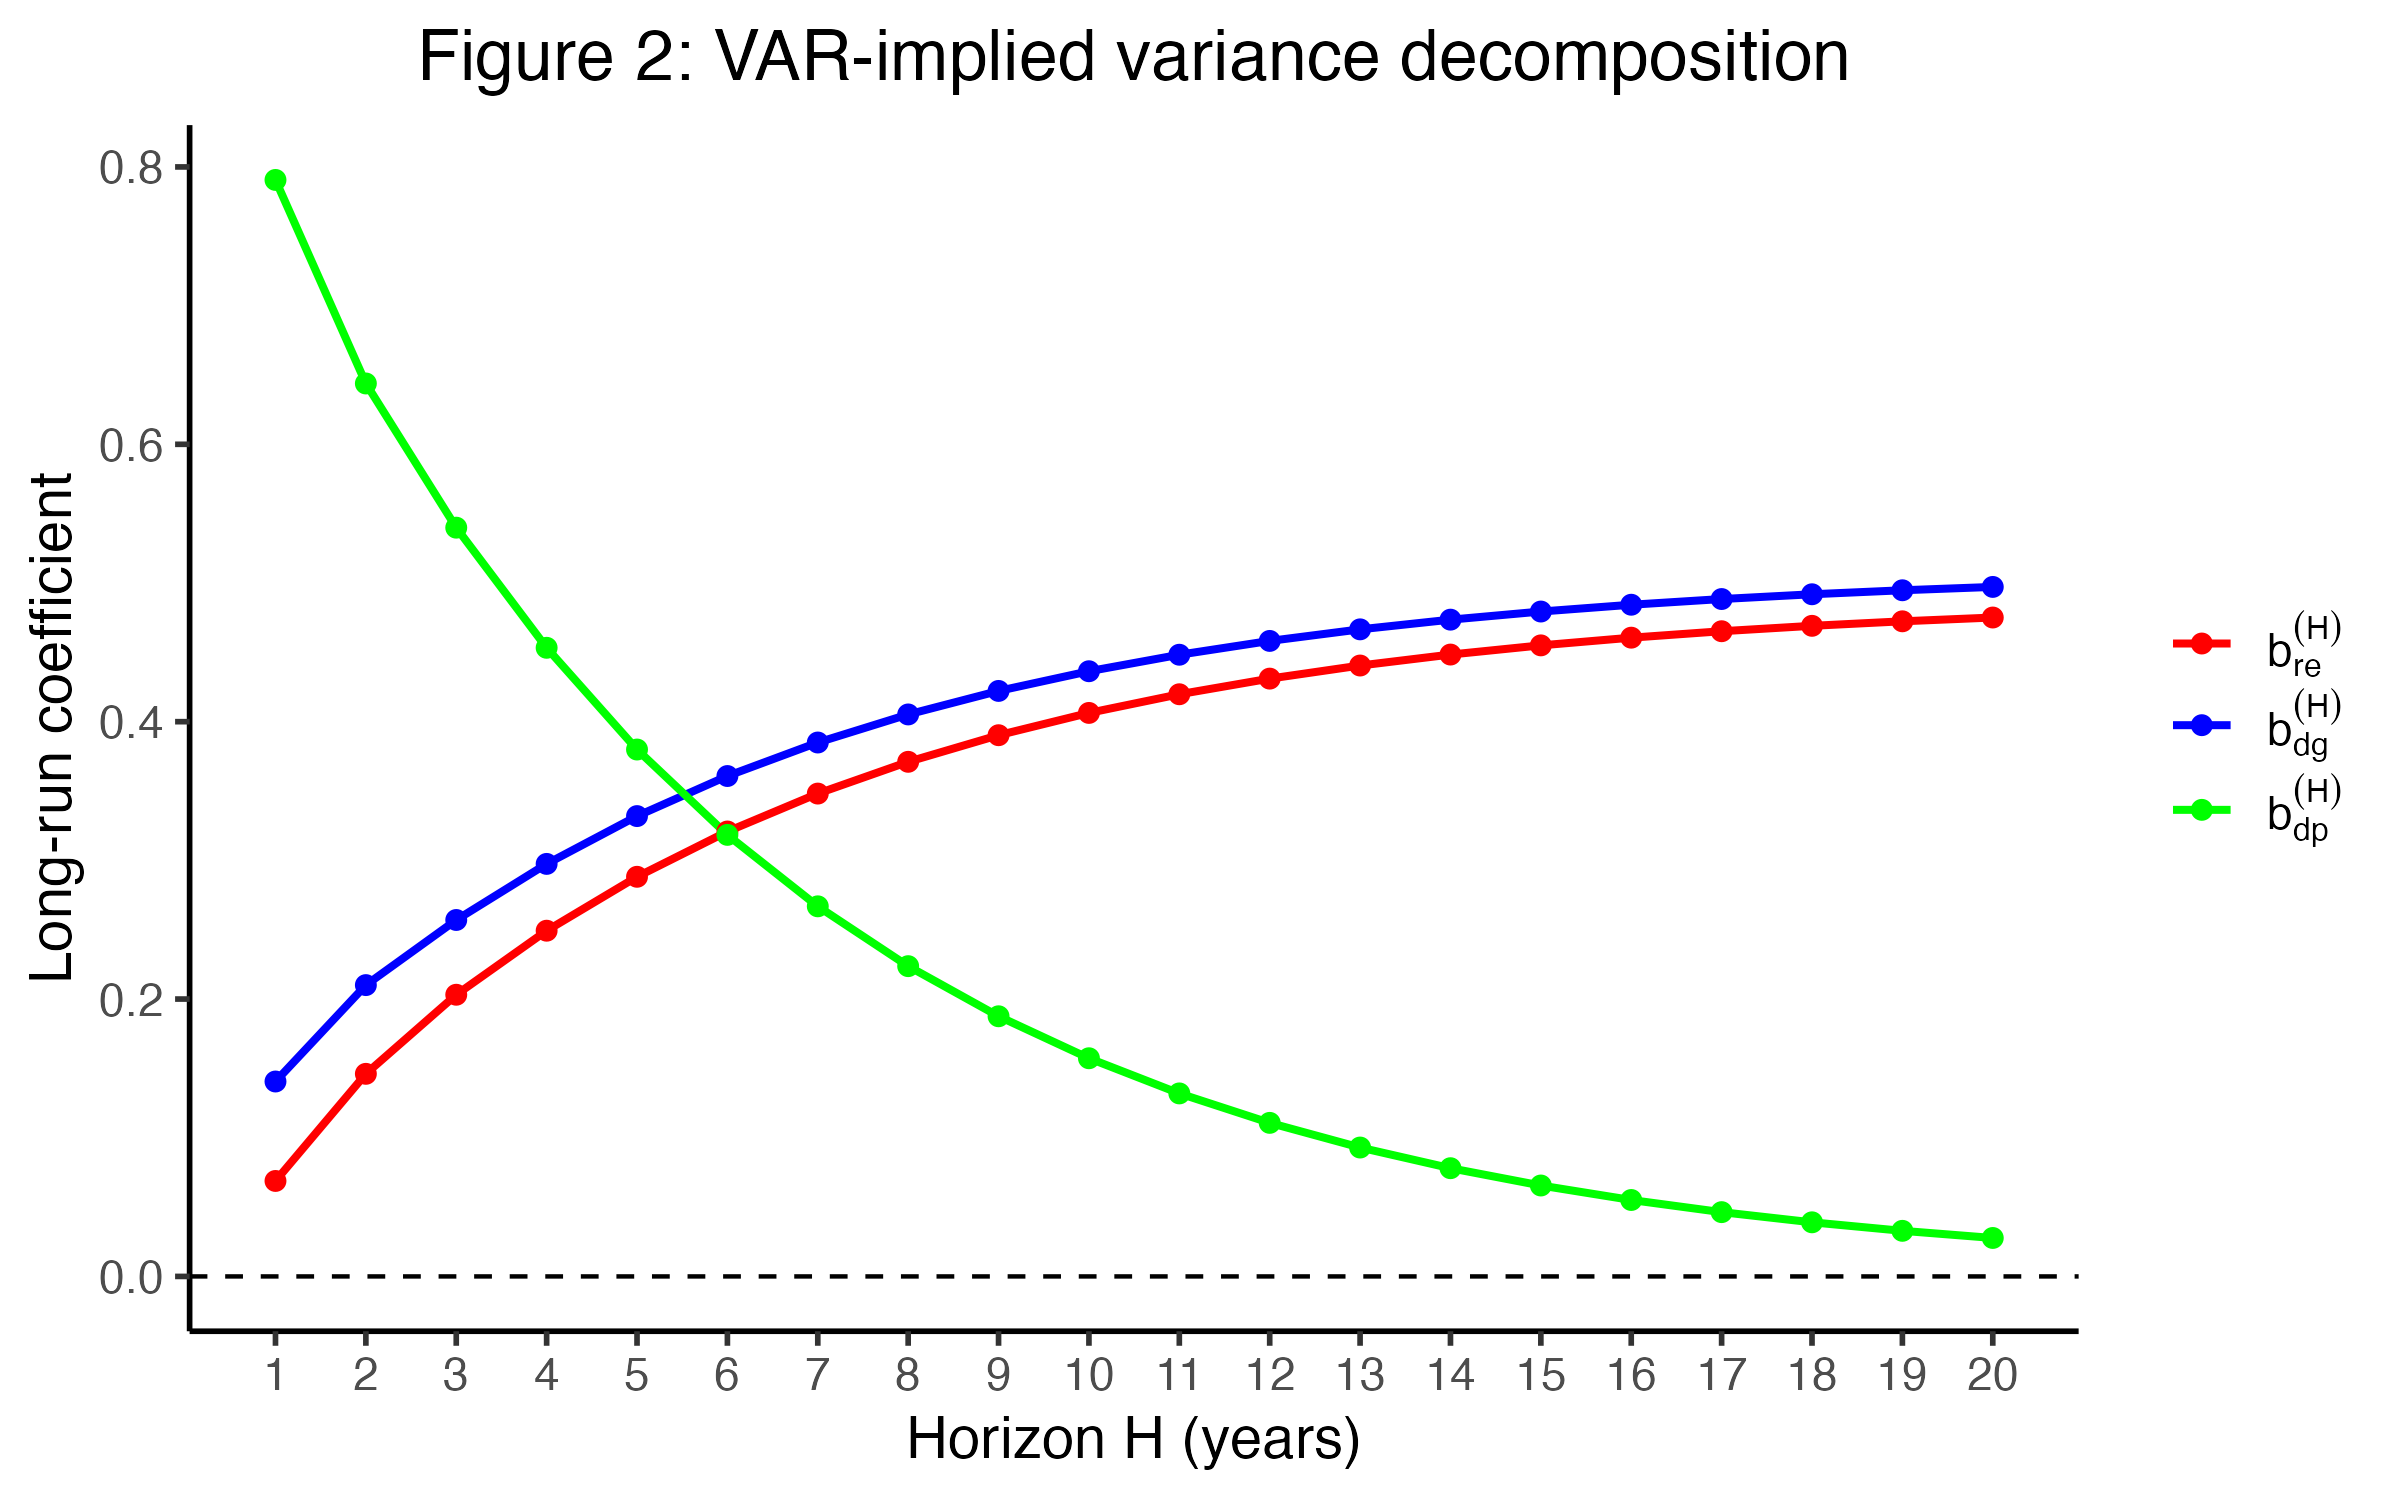
\includegraphics[width=0.6\textwidth]{figures/1c.png}
    \label{fig:q2}
\end{figure}

In particular, let $z_t = [dg_t, r_{e,t}, dp_t]$ follow $z_{t+1} = \Gamma_0 + \Gamma z_t + \varepsilon_{t+1}$ where $\varepsilon_{t+1} \overset{\mathrm{i.i.d.}}{\sim} (0,\Sigma)$. Running these overlapping annual regressions, I recover $\hat{\Gamma}$ in the form of $(z_t'z_t)^{-1}z_t'z_{t+1}$ to forecast three state variables in the future. Then, I regress $dg_t$, $re_t$, and $dp_t$ onto $dp_t$ using univariate full-sample OLS specifications to recover their coefficients in the form of the $b_z$ vector. As a result, I calculate the VAR-implied coefficients as follows:
\begin{align}
    b_{dg}^{(H)} &= -\mathbf{1}_{dg}' (\Gamma - \kappa^{H} \cdot \Gamma^{H+1}) (I - \kappa \cdot \Gamma)^{-1} b_z, \notag  \\
    b_{re}^{(H)} &= \mathbf{1}_{re}' (\Gamma - \kappa^{H} \cdot \Gamma^{H+1}) (I - \kappa \cdot \Gamma)^{-1} b_z, \notag  \\
    b_{dp}^{(H)} &= 1 - b_{dg}^{(H)} - b_{re}^{(H)} \notag 
\end{align}

\subsection*{1 (d)}
Using the same VAR process in equation (1.5) and taking H to $\infty$, the term $\kappa^{H} \cdot dp_{t+H}$ should go to 0 under the no-bubble condition. However, there is still a residual VAR-implied $b_{dp}^{\infty}$, albeit minor at 0.0011919. This could be attributed to the first-order specifications of the VAR process. Otherwise, the VAR-implied covariance coefficients for the discount rate and dividend growth components are as follows:
\begin{table}[H]
  \centering
  \caption{VAR-implied infinite-horizon coefficients}
  \label{tab:q1d}
  \begin{tabular}{lr}
    \toprule
    Component & Coefficient \\
    \midrule
    $b_{re}^{(\infty)}$ & 0.489191 \\
    $b_{dg}^{(\infty)}$ & 0.509617 \\
    \bottomrule
  \end{tabular}
\end{table}

Table 1 suggests that under the VAR(1) specifications, eventually both expected return and dividend growth equally contribute to the variation in the log dividend-price ratio in the extremely long run. 

\subsection*{1 (e)}

\[
    R_{e,t+1} = \frac{P_{t+1} + D_{t+1}}{P_t}.
\]

Taking log of both sides, we have:
\begin{align}
    r_{e,t+1}
    &= \log(P_{t+1} + D_{t+1}) - p_t \notag \\
    &= \log\left(
        P_{t+1}
        + \frac{P_{t+1} \cdot D_{t+1}}{P_{t+1}}
    \right) - p_t \notag \\
    &= \log\left(
        P_{t+1}
        \left(1 + \frac{D_{t+1}}{P_{t+1}}\right)
    \right) - p_t \notag \\
    &= p_{t+1}
    + \underbrace{
        \log\left(1 + \frac{D_{t+1}}{P_{t+1}}\right)
    }_{\equiv\,dy_{t+1}}
    - p_t
    \tag*{\color{red}(1.4)}
\end{align}

We also have:
\begin{equation*}
    dy_t
    = \log\left(1 + \frac{D_t}{P_t}\right)
    = \log\left(1 + \frac{e^{d_t}}{e^{p_t}}\right)
    = \log(1 + e^{dp_t}) \notag 
\end{equation*}


\begin{flalign}
&\Rightarrow\quad 
-dy_t
= -\log(1 + e^{dp_t})
= \log(1 + e^{dp_t})^{-1} 
&&\notag \\
%
&\Rightarrow\quad 
e^{-dy_t}
= e^{\log(1 + e^{dp_t})^{-1}}
= \frac{1}{1 + e^{dp_t}} 
&&\notag \\
%
&\Rightarrow\quad 
\frac{1}{e^{-dy_t}} - 1
= e^{dp_t} 
&&\notag \\
%
&\Rightarrow\quad
\frac{1 - e^{-dy_t}}{e^{-dy_t}}
= e^{dp_t} 
&&\notag \\
%
&\Rightarrow\quad 
1 - e^{-dy_t}
= e^{dp_t} \cdot e^{-dy_t} 
&&\notag \\
%
&\Rightarrow\quad 
\log(1 - e^{-dy_t})
= dp_t - dy_t
&&\tag*{\color{red}(1.5)}
\end{flalign}



Rewriting Equation {\color{red}(1.4)} and plugging in Equation
{\color{red}(1.5)}, we have:
\begin{align}
    r_{e,t+1} - (d_{t+1} - d_t)
    &= (d_t - p_t)
    - (d_{t+1} - p_{t+1})
    + dy_{t+1} \notag \\
    \Rightarrow\quad
    r_{e,t+1} - \Delta d_{t+1}
    &= dp_t - dp_{t+1} + dy_{t+1} \notag \\
    &= (dp_t - dy_t)
    - (dp_{t+1} - dy_{t+1})
    + dy_t \notag \\
    &= \log(1 - e^{-dy_t})
    - \log(1 - e^{-dy_{t+1}})
    + dy_t
    \tag*{\color{red}(1.6)}
\end{align}

Applying a first-order Taylor approximation to
$\log(1-e^{-dy_t})$ around $\overline{dy}$, we have:
\begin{align}
    \log(1-e^{-dy_t})
    &= f(dy_t)
    \approx f(\overline{dy})
    + f'(\overline{dy})(dy_t-\overline{dy}).
    \notag
\end{align}

Define $\kappa\equiv e^{-\overline{dy}}$. We have the following:
\begin{align}
    f(\overline{dy})
    &= \log(1-e^{-\overline{dy}})
    = \log(1-\kappa), \notag \\
    f'(\overline{dy})
    &= \frac{1}{1-e^{-\overline{dy}}}
    \cdot e^{-\overline{dy}}
    = \frac{e^{-\overline{dy}}}{1-e^{-\overline{dy}}}
    = \frac{\kappa}{1-\kappa}.
    \notag
\end{align}

As a result,
\begin{align}
    f(dy_t)
    &= \log(1-\kappa)
    + \frac{\kappa}{1-\kappa}(dy_t-\overline{dy}).
    \notag
\end{align}

Similarly,
\begin{align}
    f(dy_{t+1})
    &= \log(1-\kappa)
    + \frac{\kappa}{1-\kappa}(dy_{t+1}-\overline{dy}).
    \notag
\end{align}

Plugging these two equations into Equation {\color{red}(1.6)}, we have:
\begin{align}
    r_{e,t+1}-\Delta d_{t+1}
    &= \log(1-\kappa)
    + \frac{\kappa}{1-\kappa}(dy_t-\overline{dy})
    - \log(1-\kappa)
    - \frac{\kappa}{1-\kappa}(dy_{t+1}-\overline{dy})
    + dy_t \notag \\
    &= \frac{\kappa}{1-\kappa}(dy_t-dy_{t+1})+dy_t
    \notag \\
    &= \frac{\kappa+1-\kappa}{1-\kappa}dy_t
    - \frac{\kappa}{1-\kappa}dy_{t+1} \notag \\
    &= \frac{1}{1-\kappa}dy_t
    - \frac{\kappa}{1-\kappa}dy_{t+1} \notag \\
    &= \frac{dy_t-\kappa dy_{t+1}}{1-\kappa}.
    \notag
\end{align}
Rearraning the terms, we have: 
\begin{align}
    dy_t
    &= (1-\kappa)(r_{e,t+1}-\Delta d_{t+1})
    + \kappa dy_{t+1}
    \notag
\end{align}

Recursively substituting $dy_{t+h}$, we have:
\begin{align}
    dy_t
    &= (1-\kappa)\cdot
    \left[
        \sum_{h=1}^{H}\kappa^{h-1}\cdot r_{e,t+h}
        - \sum_{h=1}^{H}\kappa^{h-1}\cdot\Delta d_{t+h}
    \right]
    + \kappa^H\cdot dy_{t+H}
    \tag*{\color{red}(1.7)}
\end{align}

Taking the conditional expectation of both sides and assuming that
$\mathbb{E}_t[X]=X$, we have:
\begin{align}
    dy_t
    &= (1-\kappa)\cdot
    \left[
        \sum_{h=1}^{H}\kappa^{h-1}
        \cdot\mathbb{E}_t[r_{e,t+h}]
        - \sum_{h=1}^{H}\kappa^{h-1}
        \cdot\mathbb{E}_t[\Delta d_{t+h}]
    \right]
    + \kappa^H\cdot dy_{t+H}
    \tag*{\color{red}(1.8)}
\end{align}

Knowing that $0<\kappa<1$ by construction and assuming that the
no-bubble condition holds such that
$\lim_{H\to\infty}\kappa^H\cdot dy_{t+H}=0$, we let
$H\to\infty$ in Equation {\color{red}(1.8)} and have:
\begin{align}
    dy_t
    &= (1-\kappa)\cdot
    \left[
        \sum_{h=1}^{\infty}\kappa^{h-1}
        \cdot\mathbb{E}_t[r_{e,t+h}]
        - \sum_{h=1}^{\infty}\kappa^{h-1}
        \cdot\mathbb{E}_t[\Delta d_{t+h}]
    \right]
    \tag*{\color{red}(1.9)}
\end{align}

\section*{Question 2}
\subsection*{2 (a)}
Running OLS regressions of average excess return on dividend-price ratio presents the following figure. 
\begin{figure}[H]
    \centering
    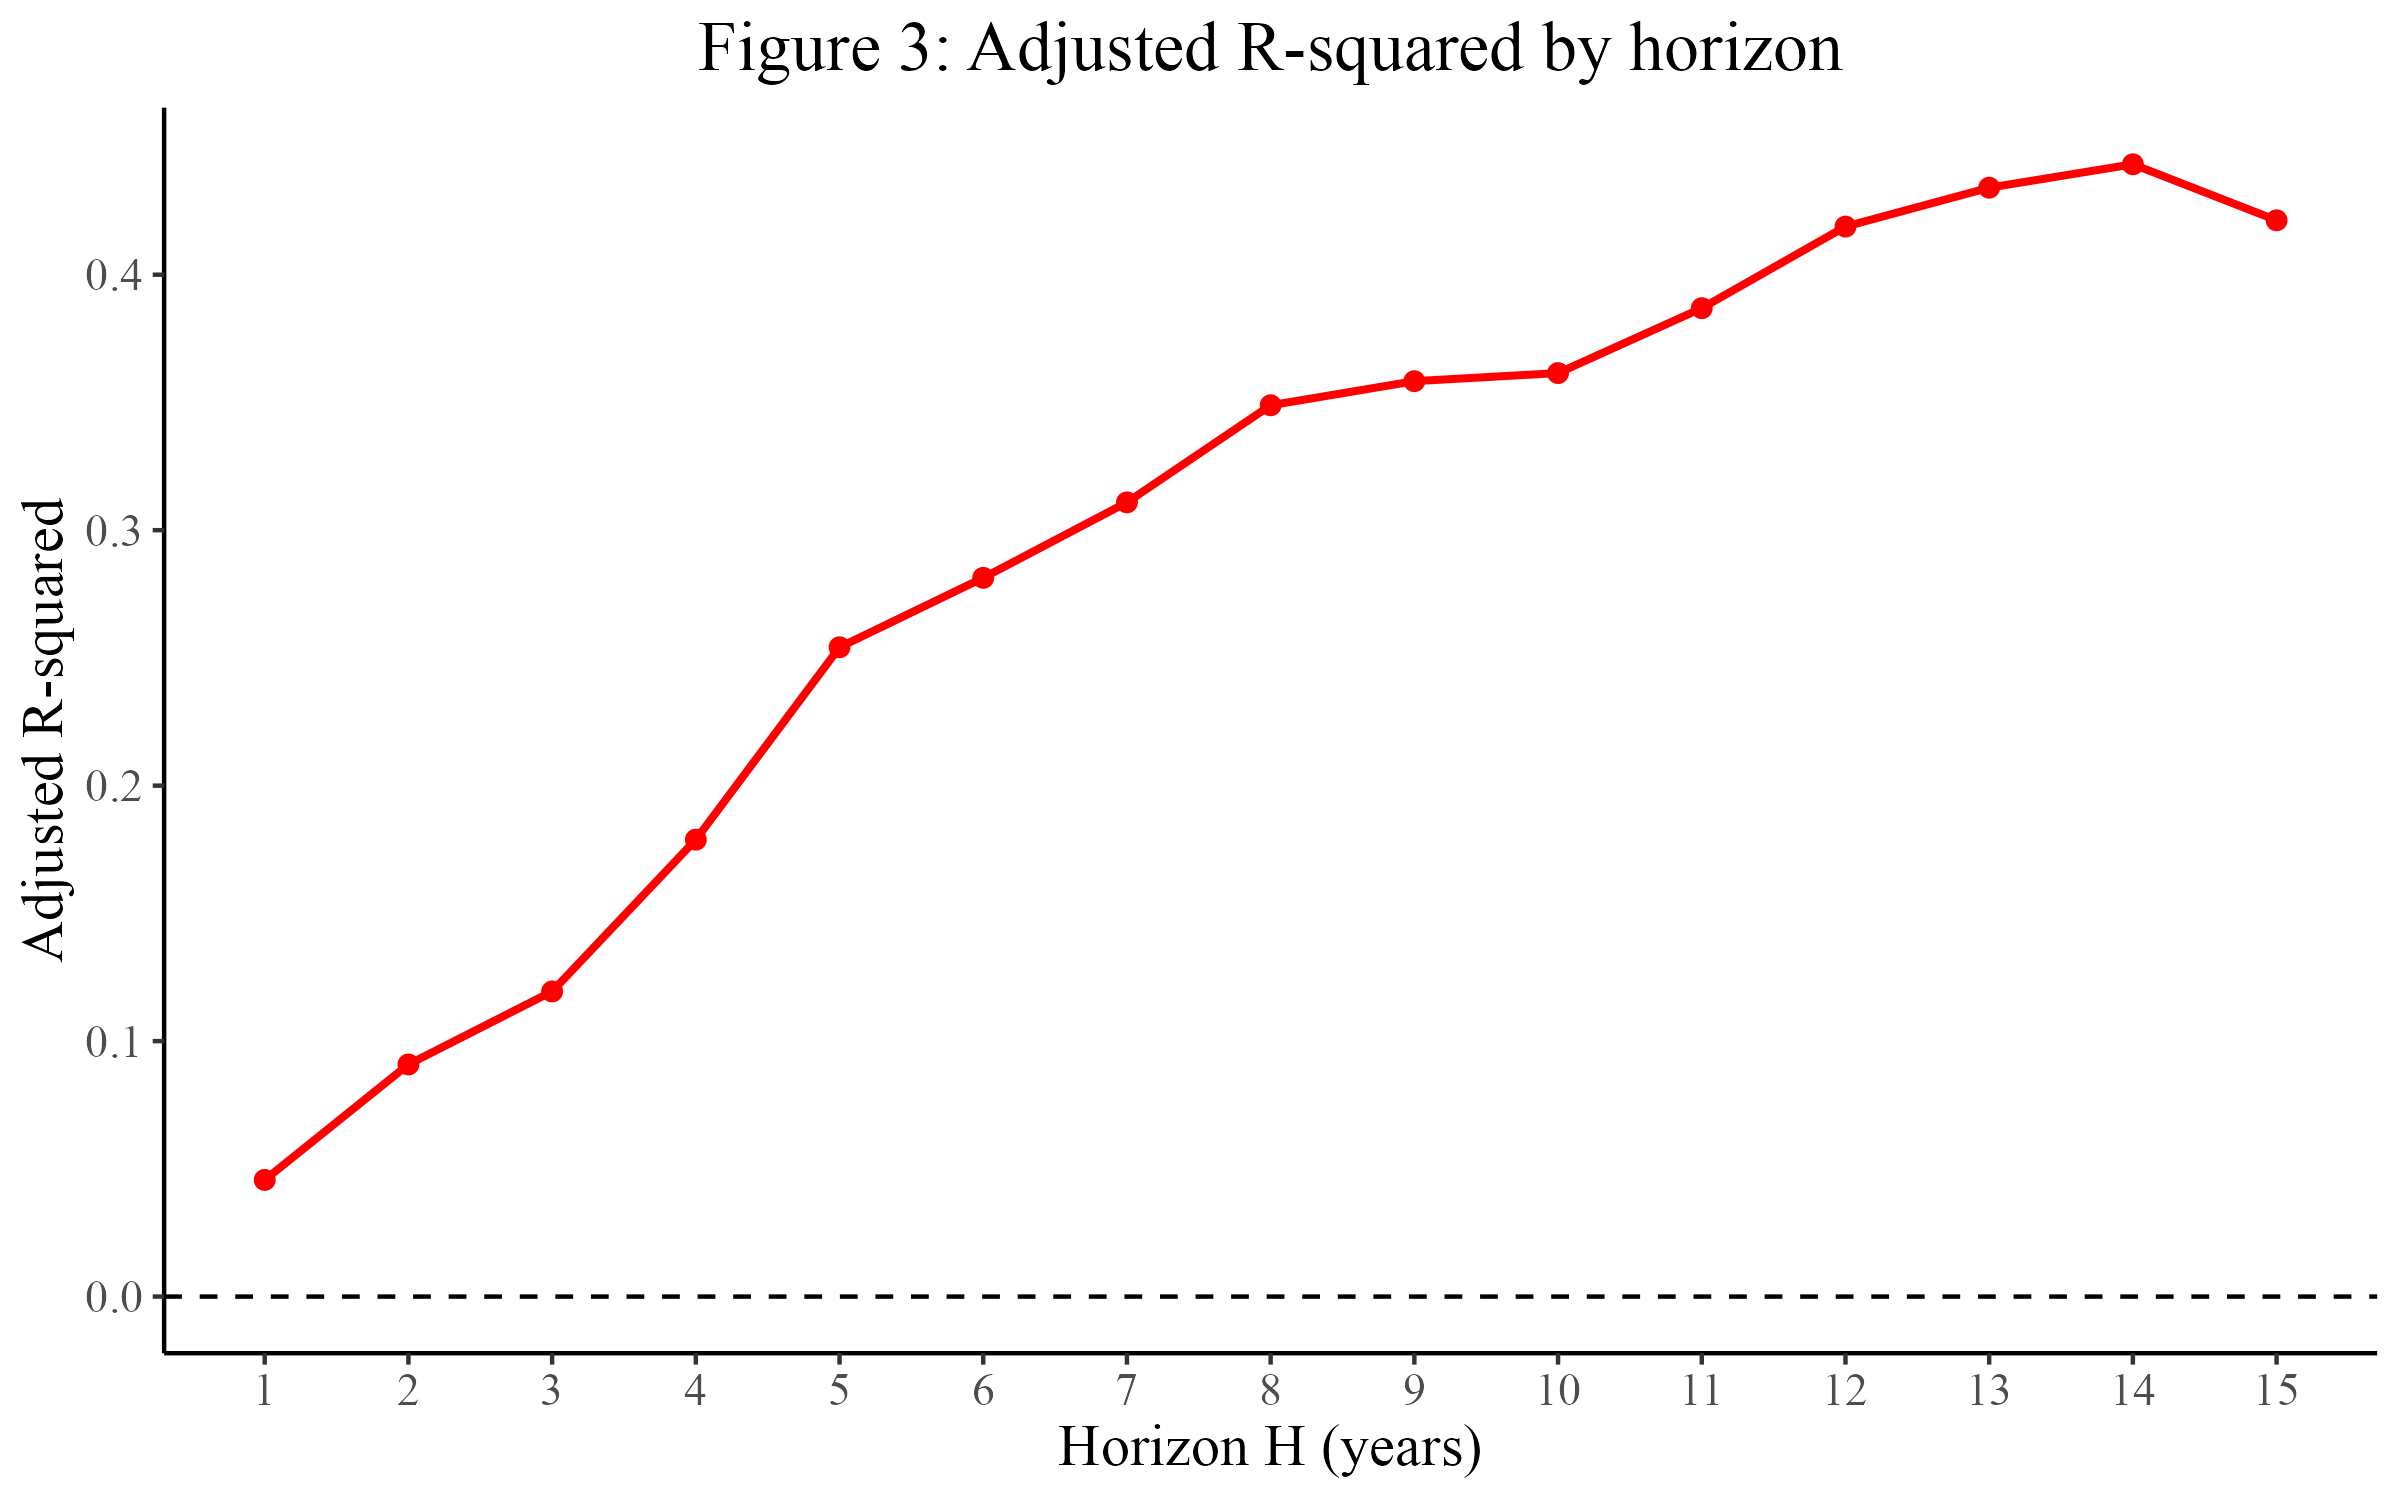
\includegraphics[width=0.6\textwidth]{figures/2a.png}
    \label{fig:q3}
\end{figure}

For the first few horizons, $R_{adj}^{2}$ remained low around 0.2, suggesting the dividend-price ratio's weak ability to predict average excess return in the short run. However, as the horizons extend, $R_{adj}^{2}$ gradually improves and reaches a peak of approximately 0.45 at H = 14. This means that over the longer horizon, current dividend-price ratio explains about 45\% of the variation in the long-run average excess return, rendering this independent variable relevant in predicting long-term return. 

\subsection*{2 (b)}

I estimated the one-year OLS regression of excess return on current dividend-price ratio and retrieved the fixed estimated $\hat{b}$ and $\hat{e}$: 
\begin{align*}
xR_{e,t+1} &= a + b \cdot D_{t}/P_{t} + e_{t} 
\end{align*}

For each estimator, I calculated a corresponding spectral density matrix $\hat{S}$ before feeding it into the following sandwich covariance matrix estimator: 
\begin{align*}
\widehat{\operatorname{Avar}}(\hat{\theta})
= \frac{1}{T} 
Q^{-1}\widehat{S}Q^{-1}, 
\qquad Q= \frac{1}{T}X'X
\end{align*}

Taking square root of the diagonal entries of the coefficient covariance matrix, I derive the following table: 
\begin{table}[H]
  \centering
  \caption{Predictive-regression coefficient estimates and standard errors}
  \label{tab:q2b}
  \begin{tabular}{lrrr}
    \toprule
    Method & $\hat{b}$ & Std. Error & $t$-stat \\
    \midrule
    OLS & 2.8038 & 0.3802 & 7.3754 \\
    White (1980) & 2.8038 & 0.6587 & 4.2569 \\
    Newey--West (1987), 11 lags & 2.8038 & 1.2990 & 2.1584 \\
    Hansen--Hodrick (1980), 11 lags & 2.8038 & 1.4537 & 1.9287 \\
    Newey--West (1987, 1994), automatic (22 lags) & 2.8038 & 1.2523 & 2.2390 \\
    \bottomrule
  \end{tabular}
\end{table}

As the estimate accounts for both heteroskedasticity and autocorrelation, the standard error becomes larger and the t-stat declines. 

\subsection*{2 (c)} 
The Amihud and Hurvich (2004) correction responds to Stambaugh's concern for bias in the coefficient estimate due to the persistent nature of the predictor, or $\frac{D_t}{P_t}$ in this case. Indeed, estimating the AR(1) regression of $D_{t+1}/P_{t+1}$ on $D_t/P_t$  such that $D_{t+1}/ P_{t+1} = \theta + \phi \cdot D_t/P_t + u_{t+1} $, I retrieved $\hat{\phi} = 0.7197$, suggesting that shocks to dividend-price ratio disappear verly slowly. Given our finite sample, the OLS estimate of the persistence coefficient tends to be biased downward so that $\mathbb{E}_t[\hat{\phi} - \phi ] < 0$. As a result, a downwardly biased $\hat{\phi}$ also leads to an upward bias in $\hat{b}$ via a negative covariance between shocks to return ($e_{t+1}$) and shocks to predictor ($u_{t+1}$). In order to correct the OLS's overstated return predictability, I re-estimate the slope coefficient using the Amihud and Hurvich (2004) correction as follows: 
\begin{enumerate}
    \item Step 1: Convert the dataset from months into the corresponding $T=95$ calendar years. Construct the the bias-corrected slope estimate $\hat{\phi}^{c} = \hat{\phi} + (1/T) \cdot (1+ 3 \cdot \hat{\phi}) + (1/T^2) \cdot 3 \cdot (1+ 3 \cdot \hat{\phi})$.
    \item Step 2: Subbing $\hat{\phi}^{c}$ into the AR(1) process, I calculate the bias-corrected residual estimate: $\hat{u}_{t+1}^{c} = D_{t+1}/ P_{t+1} - (\hat{\theta} +  \hat{\phi}^{c} \cdot D_t/P_t)$. 
    \item Step 3: I plug the updated AR(1) regression in place of $D_t/P_t$ into Equation (2.2) in part (b) and retrieve a new $\hat{b}_{AH}$: $xR_{e,t+1} = a + b_{AH} \cdot D_t/P_t + b_{u} \cdot \hat{u}_{t+1}^{c} + e_{t+1}$. 
\end{enumerate}

The slope estimates for the conventional OLS and Amihud and Hurvich are $\hat{b}$ = 2.8038 and $\hat{b}_{AH}$ = 2.3412 respectively. This empirical result is in line with the small sample bias discussion above, proving that the corrected $\hat{u}_{t+1}^{c}$ controls for the contemporaneous correlation between the return and dividend-price ratio innovations and shrinks the inflated slope coefficient.

\subsection*{2 (d)} 
The in-sample OLS forecast used the full-sample data following Equation 2.2 to derive in-sample fitted values $\hat{E}_{t}^{IS}[{xR}_{e}]$. I estimated the time-varying $a_{t}^{OS}$ and $b_{t}^{OS}$ via the OLS regression $xR_{e,t+1} =  a_{t}^{OS} + b_{t}^{OS} \cdot D_t/P_t + e_{t+1}$ using an expanding window and historical observations of $\{D_t/P_t, xR_{e,t+1}\}$ from (December 1927, December 1928) to (December 1938, December 1939). Then, I retrieved the out-of-sample forecast $\hat{E}_{t}^{OS}[{xR}_{e}]$ starting in December 1940 and using estimated coefficients and observations in December 1939. The average historical expanding-window excess return $\overline{xR}_{e,t}$ is calculated as $\overline{xR_{e,t}} = (1/N_t) \cdot \sum_{i=1}^{N_t} xR_{e,i}$ where $N_t$ denotes the number of observations available at time t. The first $\overline{xR}_{e,t}$ uses $xR_{e,i}$ from December 1928 to December 1939. 
Using the out-of-sample forecasting errors, I calculated the out-of-sample $R^{2}_{OS}$ as follows:
\[
    R^{2}_{OS}
    = 1 - 
    \frac{
    \displaystyle\sum_{t=1}^{T}
    \left( 
    xR_{e,t+1} - 
    \widehat{E}_t^{OS}\left[ xR_{e,t}\right]
    \right)^2
    }{
    \displaystyle\sum_{t=1}^{T} 
    \left(
    xR_{e,t+1} - 
    \overline{xR_{e,t}} 
    \right)^2
    }
    = -0.00611
\]

\begin{figure}[H]
    \centering
    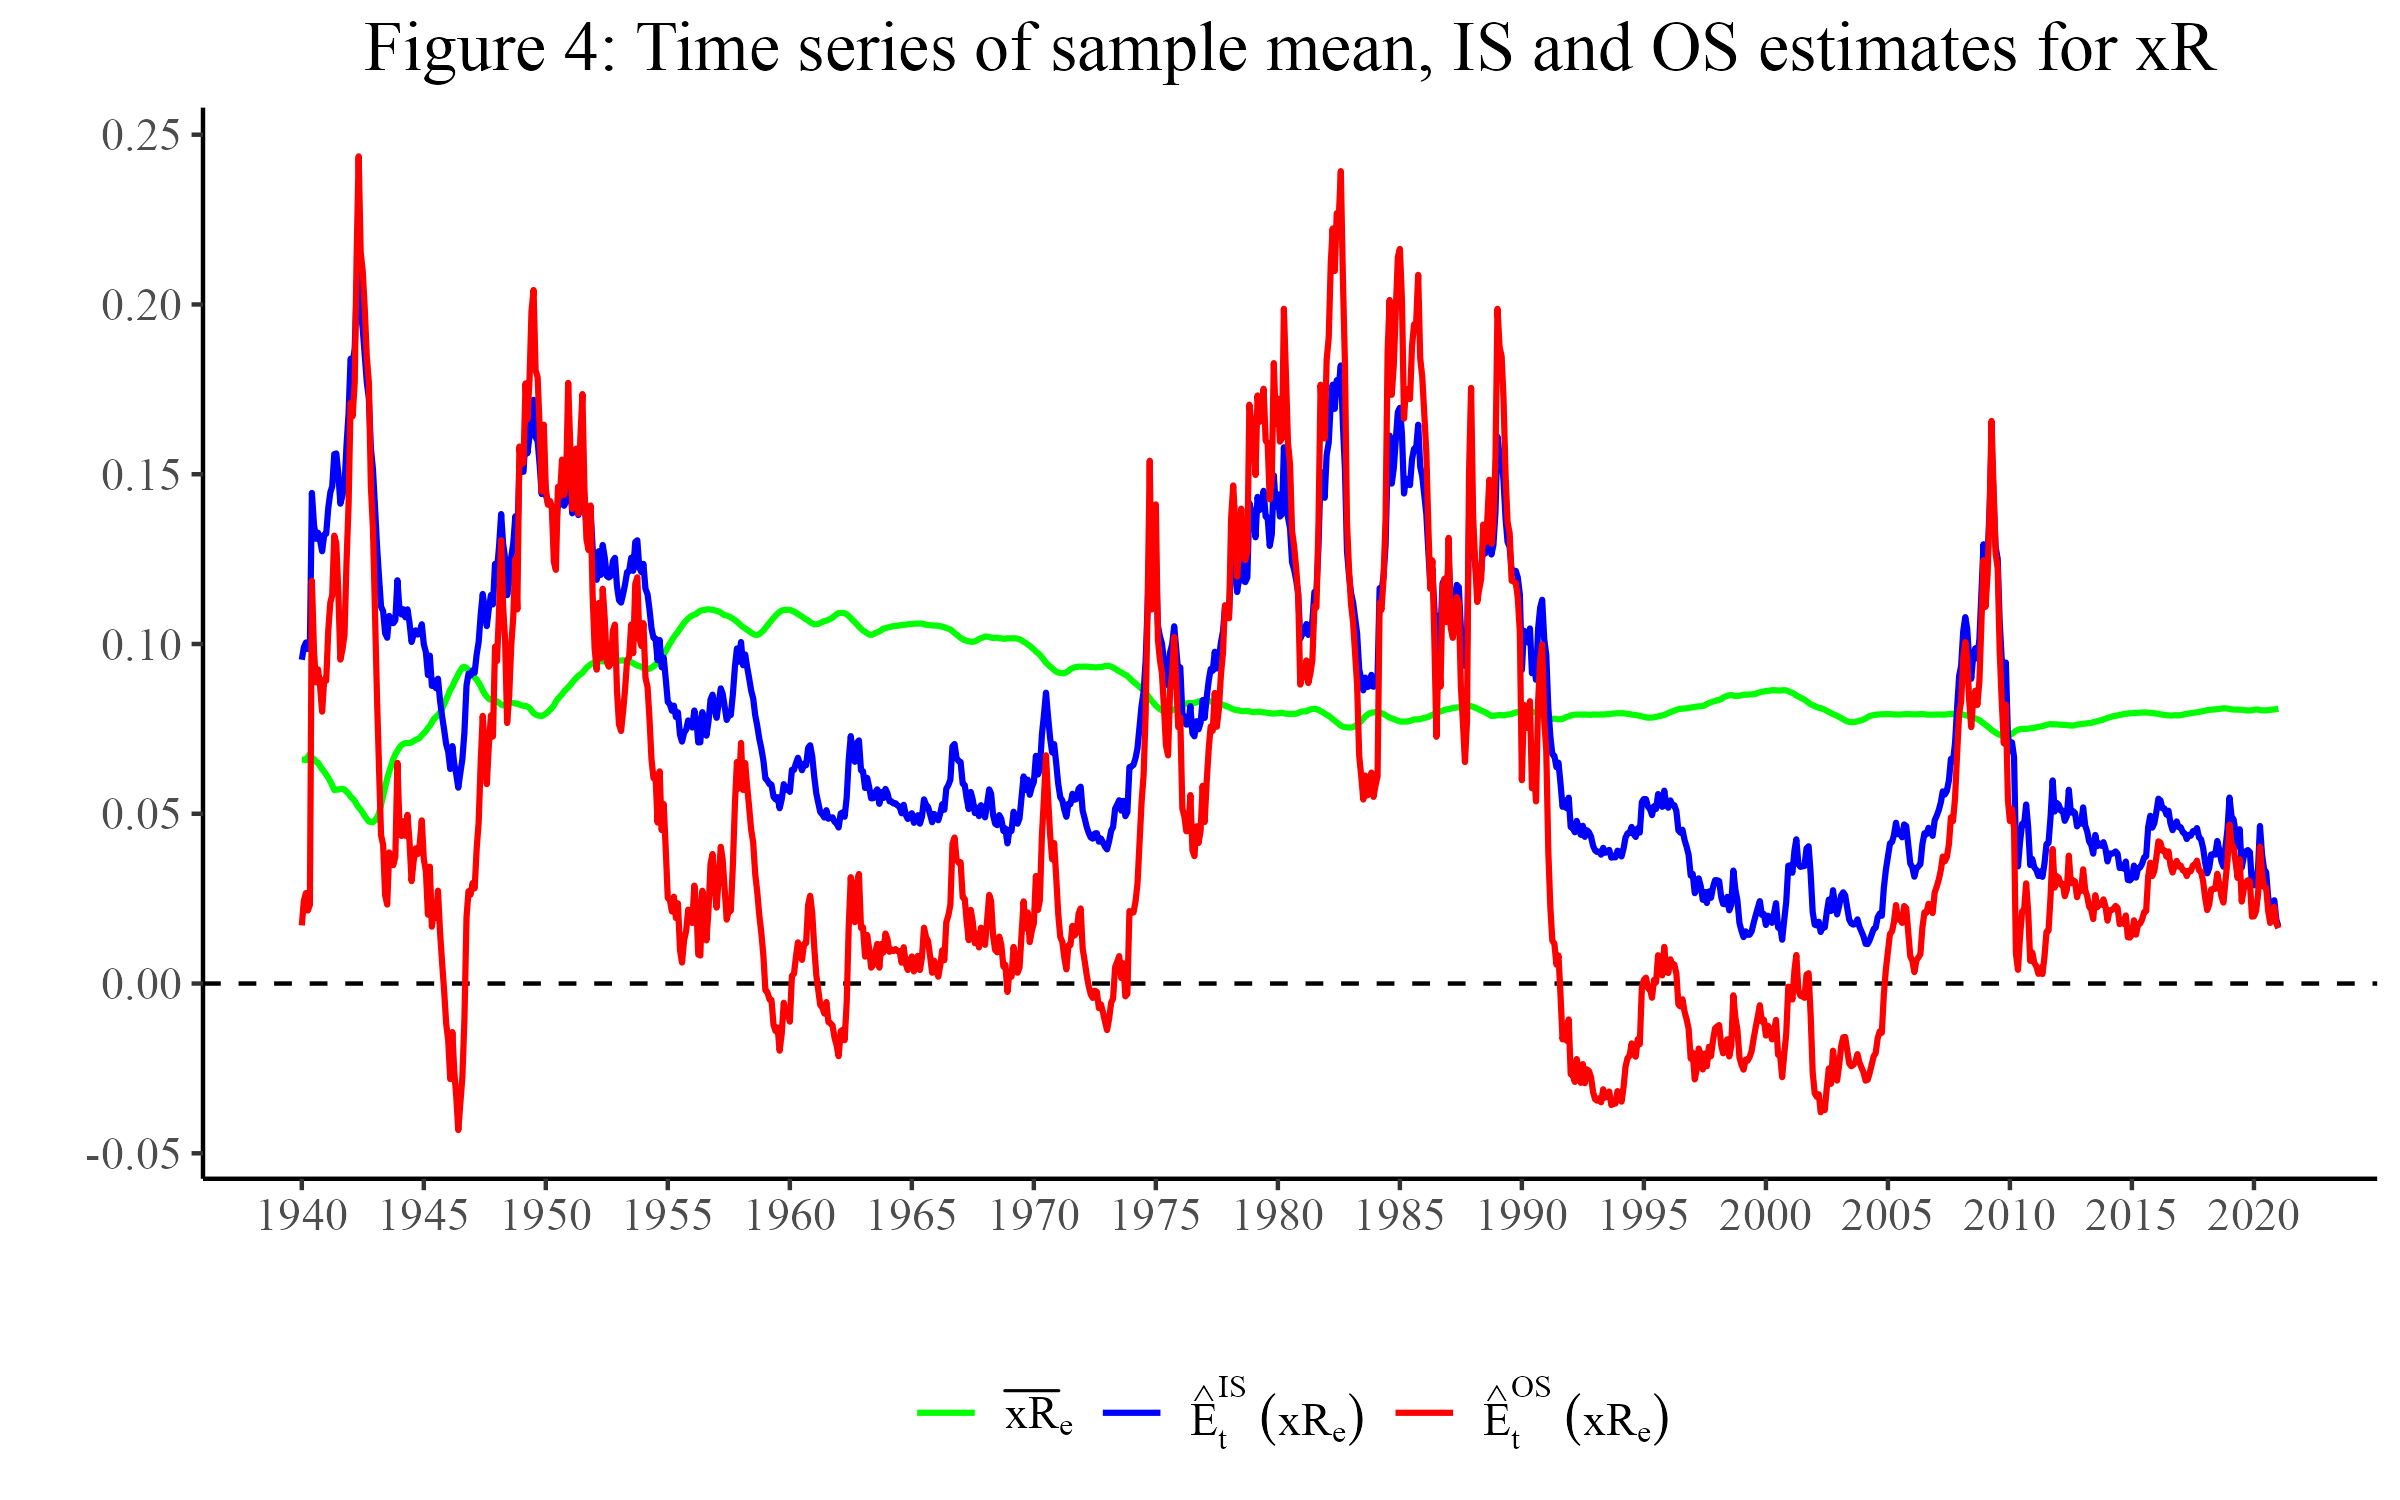
\includegraphics[width=0.75\textwidth]{figures/2d_1.png}
    \label{fig:q4}
\end{figure}

The 50-year rolling window $R^{2}_{OS}$ uses 600 observations of forecasting errors from the OS OLS estimation with the first window covering January 1941 to December 1990. As observed from the plot below, the predictability power of the model severely declines as the horizon expands, turning negative around 2000. This evidence demonstrates that the OS forecasts performed worse than the intercept-only OLS regression with an expanding window.  
\begin{figure}[H]
    \centering
    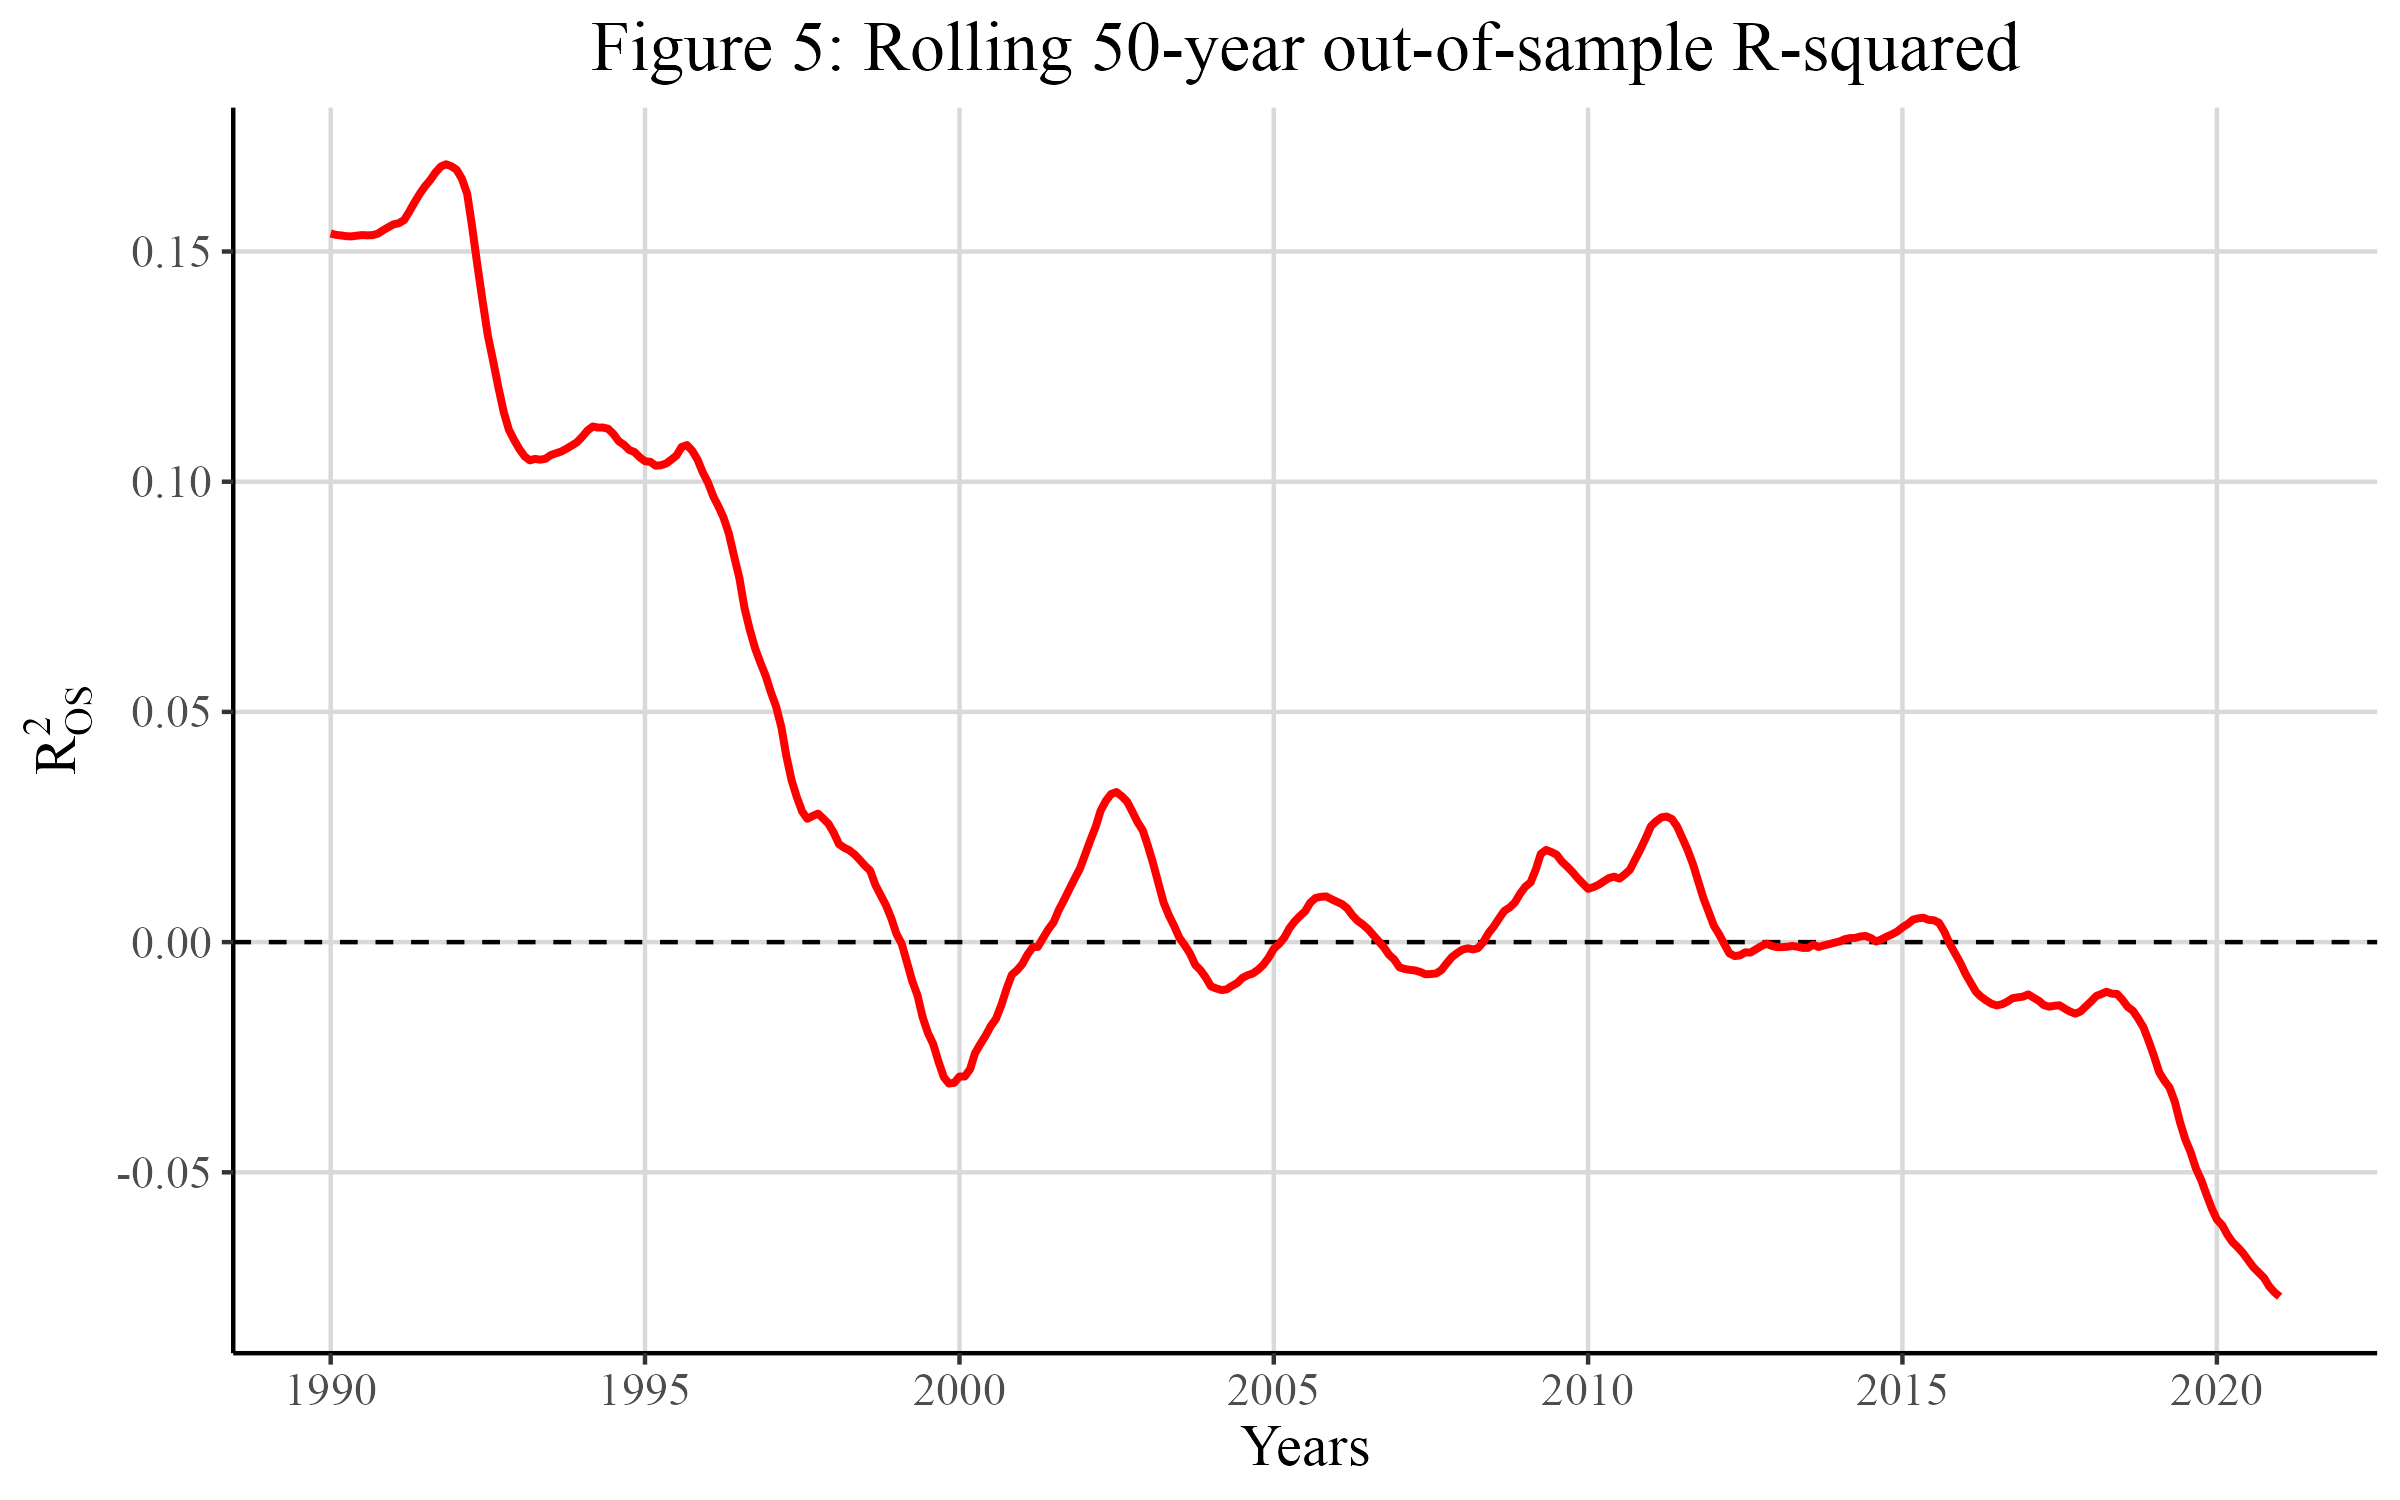
\includegraphics[width=0.75\textwidth]{figures/2d_2.png}
    \label{fig:q5}
\end{figure}

\subsection*{2 (e)} 
I keep the same $\hat{E}_{t}^{IS}[{xR}_{e}]$ and $\overline{xR}_{e,t}$ as constructed in question 2d. For the out-of-sample estimation, assuming that dividend growth is unexpected and expected return is 100\% persistent, Equation 1.9 implies:
\[
    log(1+ D_t/P_t) 
    = \mathbb{E}_{t} [r_e] - g
\]

where $\mathbb{E}_{t} [\Delta d_{t+h}] = g$ and $\mathbb{E}_{t} [\Delta r_{e,t+h}] = \mathbb{E}_{t} [r_e]$. Assuming 0\% real interest rate, $e^{rf} = 1$. Let $G_t = exp(g)$. Taking the exponent of both sides and subtracting $e^{rf}$, we have: 
\[
    xR_{e,t+1}
    = (G_t - 1) + G_t \cdot D_t/P_t
\]

Applying the steady state implied coefficients, I set $ \hat{a} = \bar{G_t} -1$ and $ \hat{b} = \bar{G_t}$ such that $\bar{G_t}$ is the average $e^{\Delta d}$ over the expanding window period (starting from December 1927), I estimate $\hat{E}_{t}^{OS2}[{xR}_{e}]$ and retrieve the following figure. 
\begin{figure}[H]
    \centering
    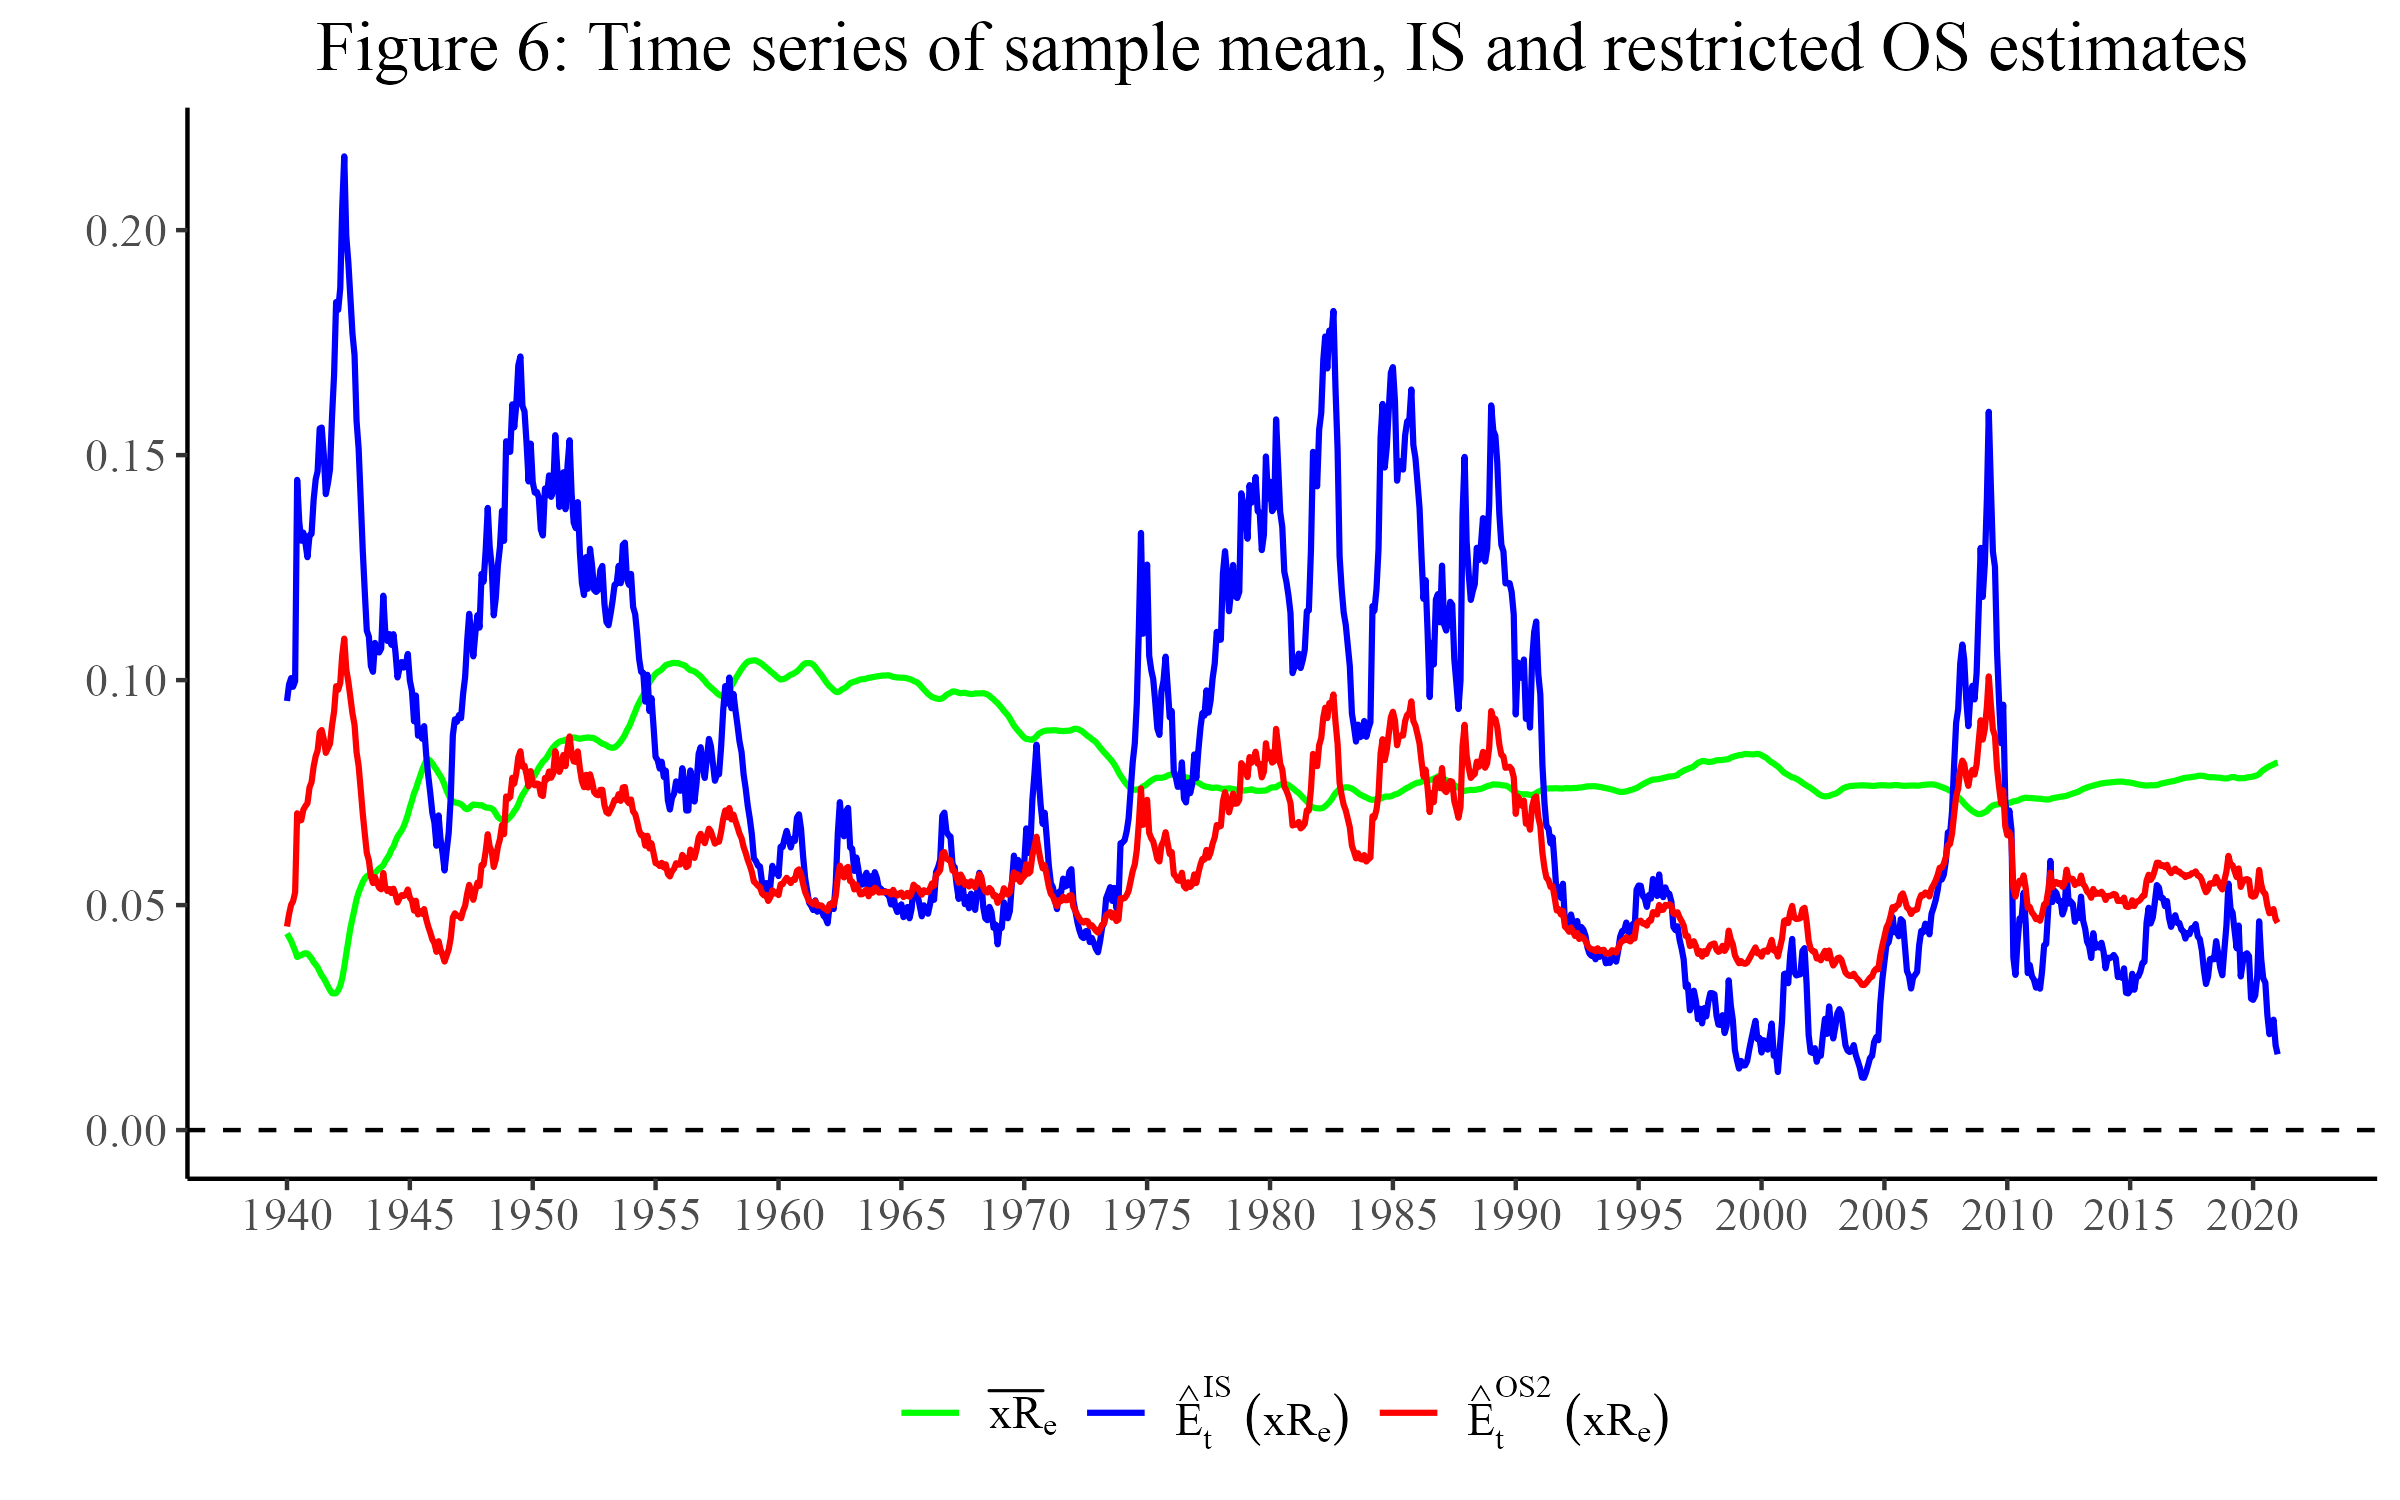
\includegraphics[width=0.75\textwidth]{figures/2e_1.png}
    \label{fig:q6}
\end{figure}

$R^{2}_{OS2}$, using the same formula as question 2d, is 0.001978 with the 50-year rolling $R^{2}_{OS2}$ time series as follows: 
\begin{figure}[H]
    \centering
    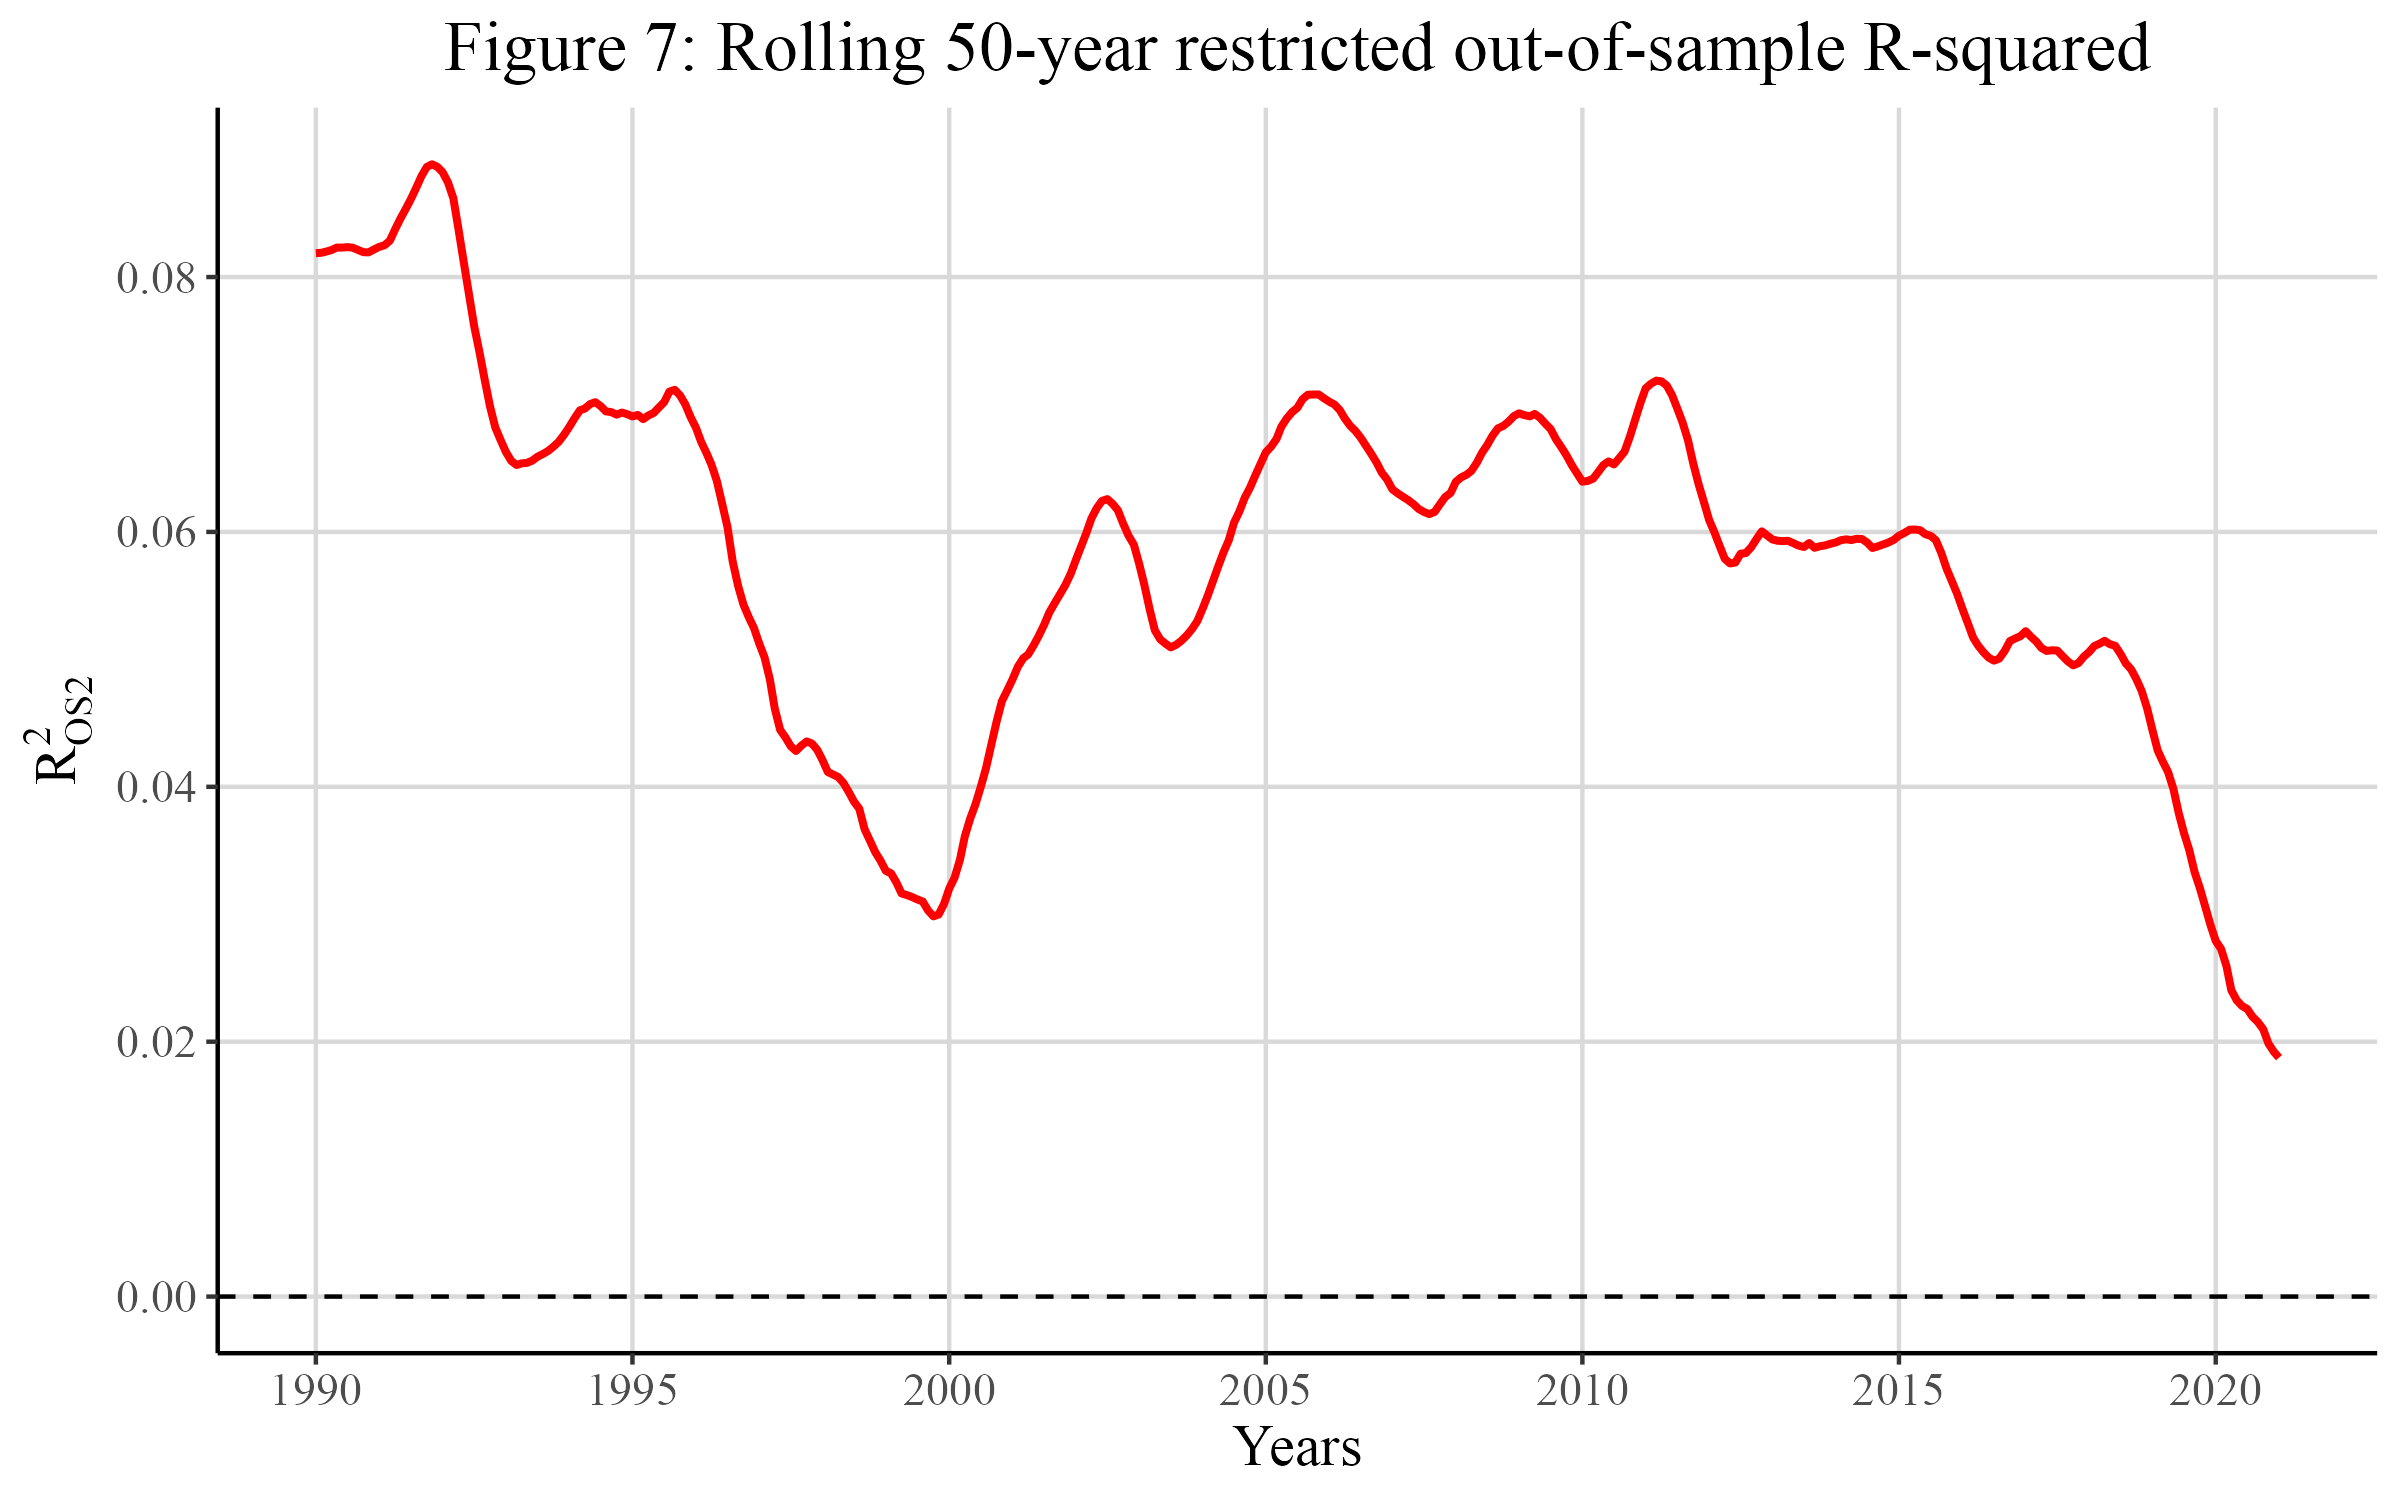
\includegraphics[width=0.75\textwidth]{figures/2e_2.png}
    \label{fig:q7}
\end{figure}

Given these results, we can clearly see that the steady state constraint has slightly improved the out-of-sample $R^2$ $(0.001978 > 0.001824)$. Looking over the horizons, the rolling $R^2$ using the fixed coefficient constraint also never dipped below 0, suggesting that imposing restrictions from steady-state valuation model can improve OS predictability. This makes sense as less estimation errors come at the expense of less flexibility in estimating regression coefficients. This conclusion is consistent with the view of Campbell \& Thompson (2008). 
    
\section*{Question 3}
\subsection*{3 (a)} 
Imposing standard restrictions, I restricted the sample of CRSP monthly stocks to contain common stocks on firms incorporated in the United States, trading on NYSE, Amex, or Nasdaq, and exclude utilities and financials. To account for delisting, I calculated the adjusted CRSP return as  $ {RET\_ADJ}_{\tau} = (1+RET_\tau)(1+DLRET_\tau)-1$. Then I constructed the monthly momentum signal for a firm $j$ at time $\tau = 1,\ldots, T$ as follows:
\[
    MOM_{j, \tau} = \prod_{t=1}^{12}  (1+ RET\_ADJ_{j,\tau - t}) - 1 
\]

To preserve the construction of MOM, I verified that for each $PERMNO$, ${RET\_ADJ}_{\tau}$ is available and that there are 12 chronologically ordered observations of ${RET\_ADJ}_{\tau}$ corresponding to 12 calender months. For companies with available $DLSTCD$ and $DLRET$, there is no subsequent obeservation. Then, I proceeded to match the newly constructed CRSP sample with the Chen \& Zimmermann (2022) Mom12m dataset on $PERMNO$ and $YYYYMM$. Using an inner merge, I retrieved 2,410,492 pairs of $MOM$ and $MOM\_CZ$ and ran 739 monthly cross-firm regressions in the sample as follows:
\[
    MOM\_CZ_{j, \tau} = a_\tau + b_\tau \cdot MOM_{j, \tau} + e_{j, \tau}
\]

\begin{figure}[H]
    \centering
    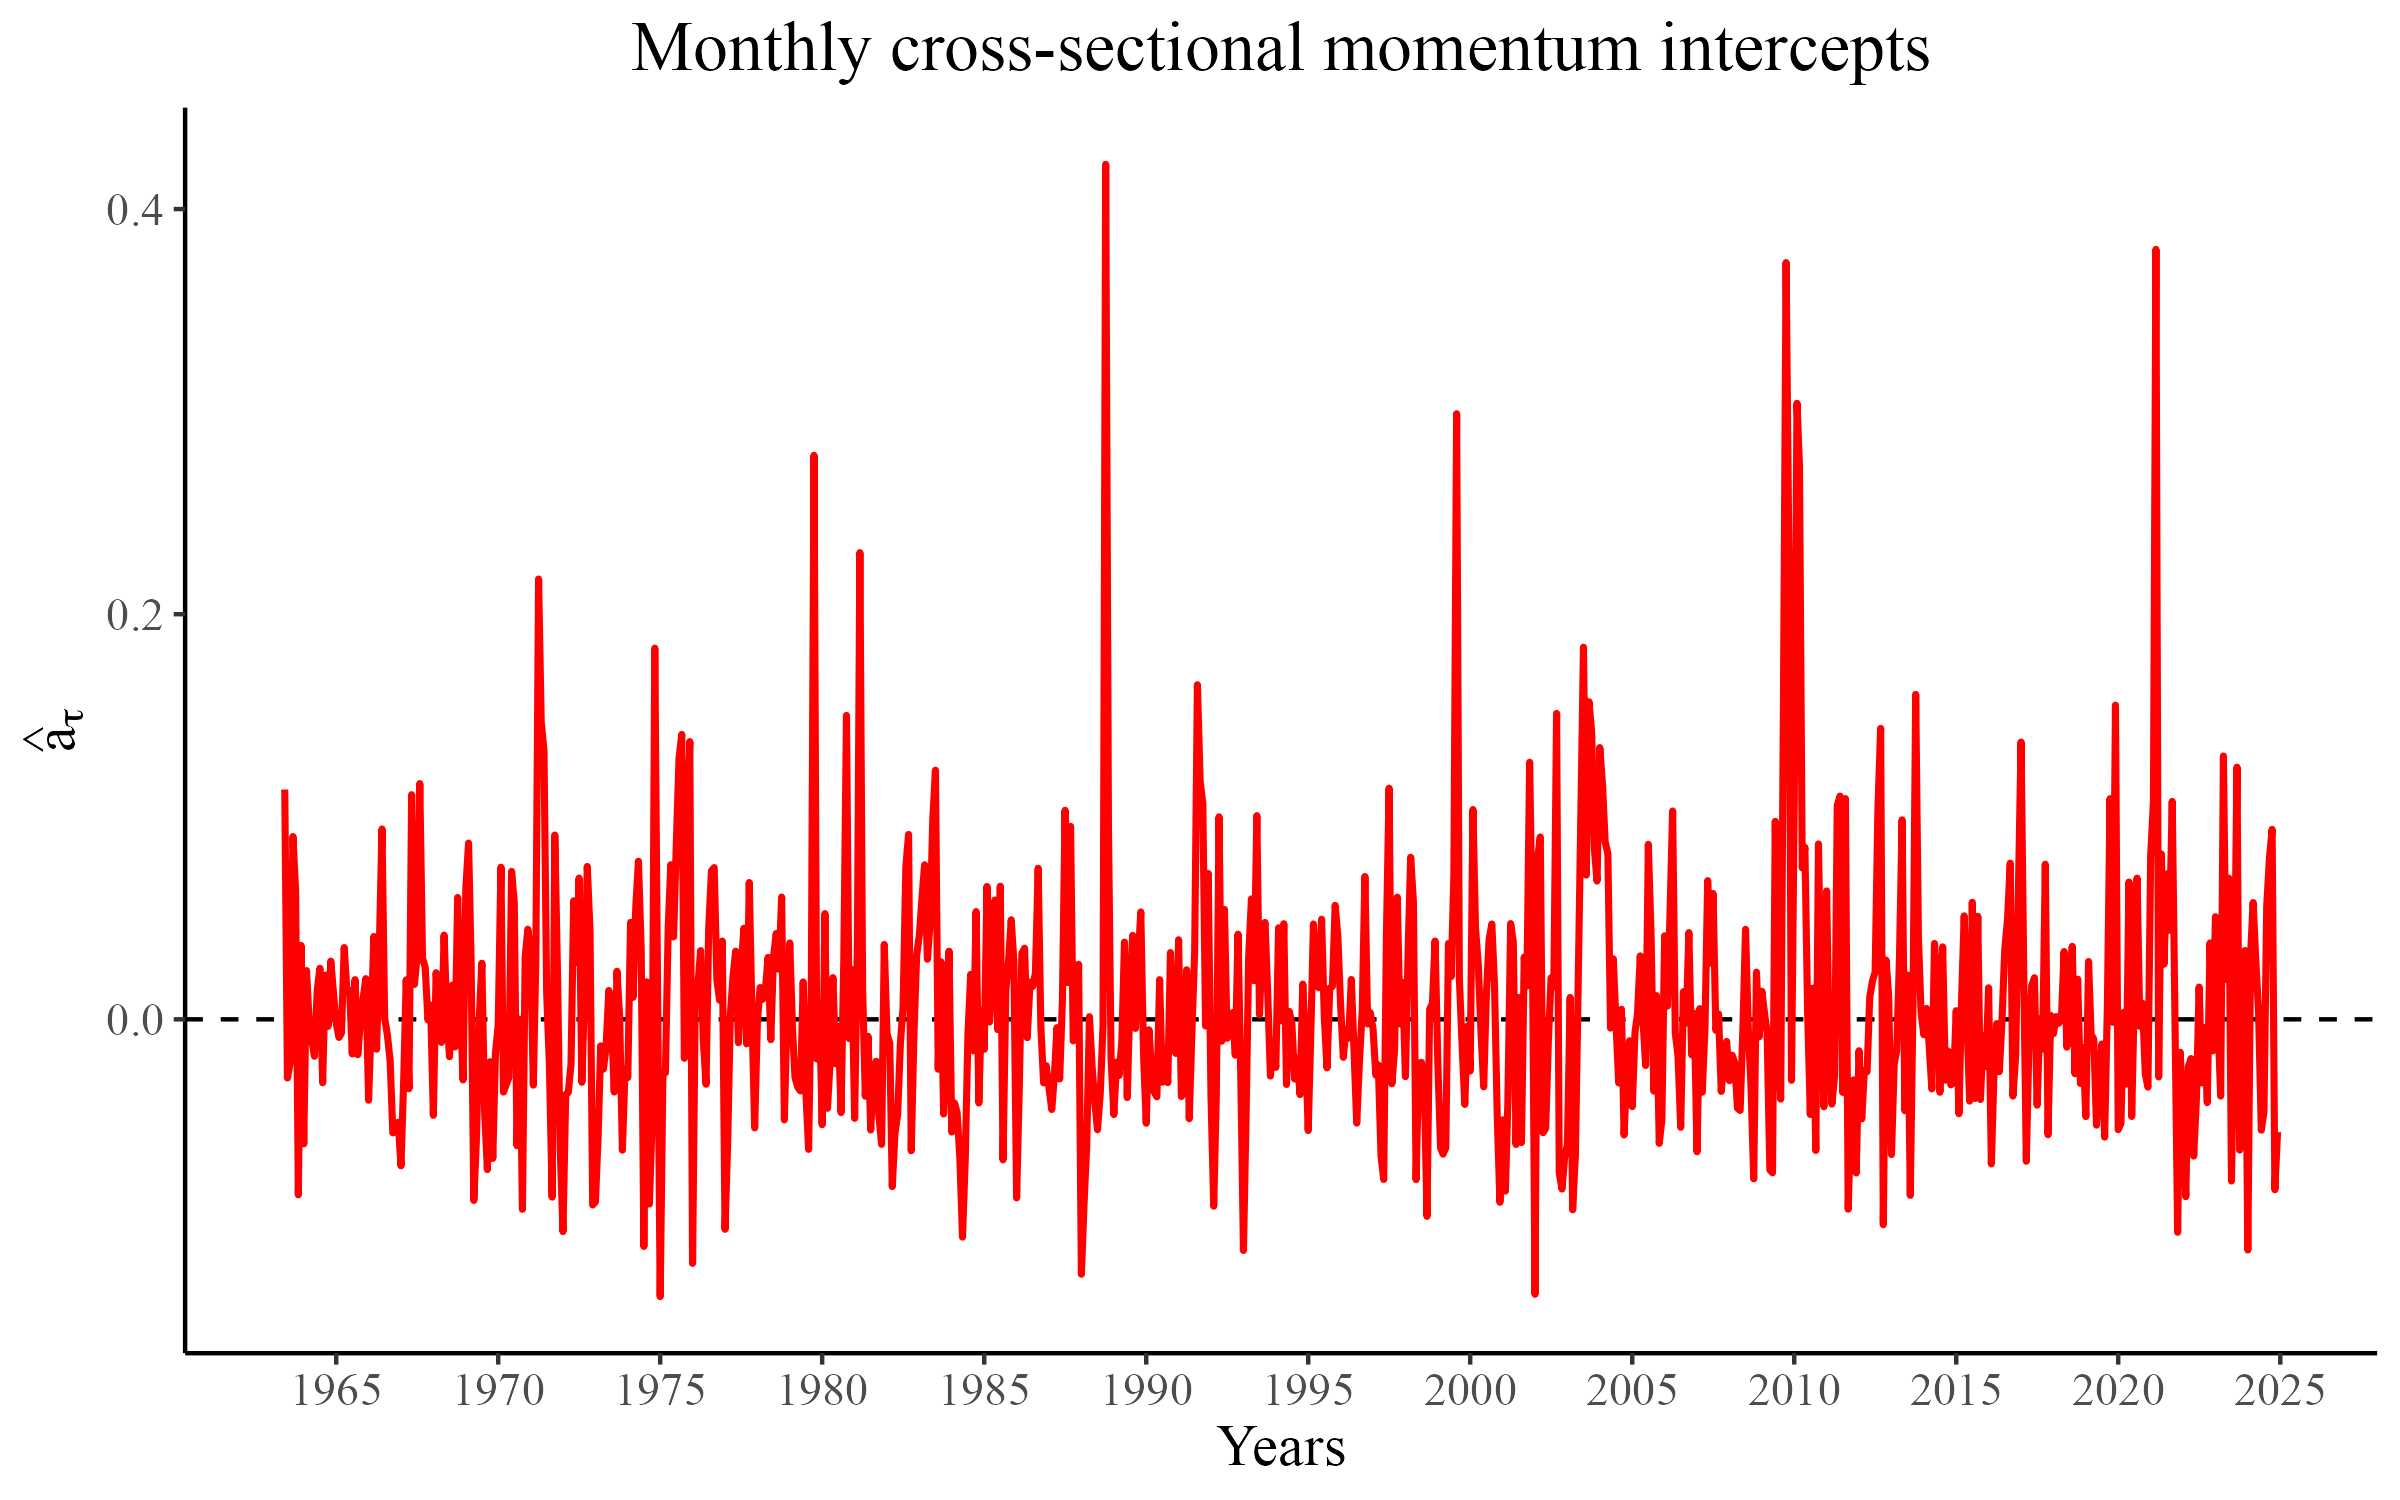
\includegraphics[width=0.75\textwidth]{figures/3a_intercept.png}
    \label{fig:q12}
\end{figure}

\begin{figure}[H]
    \centering
    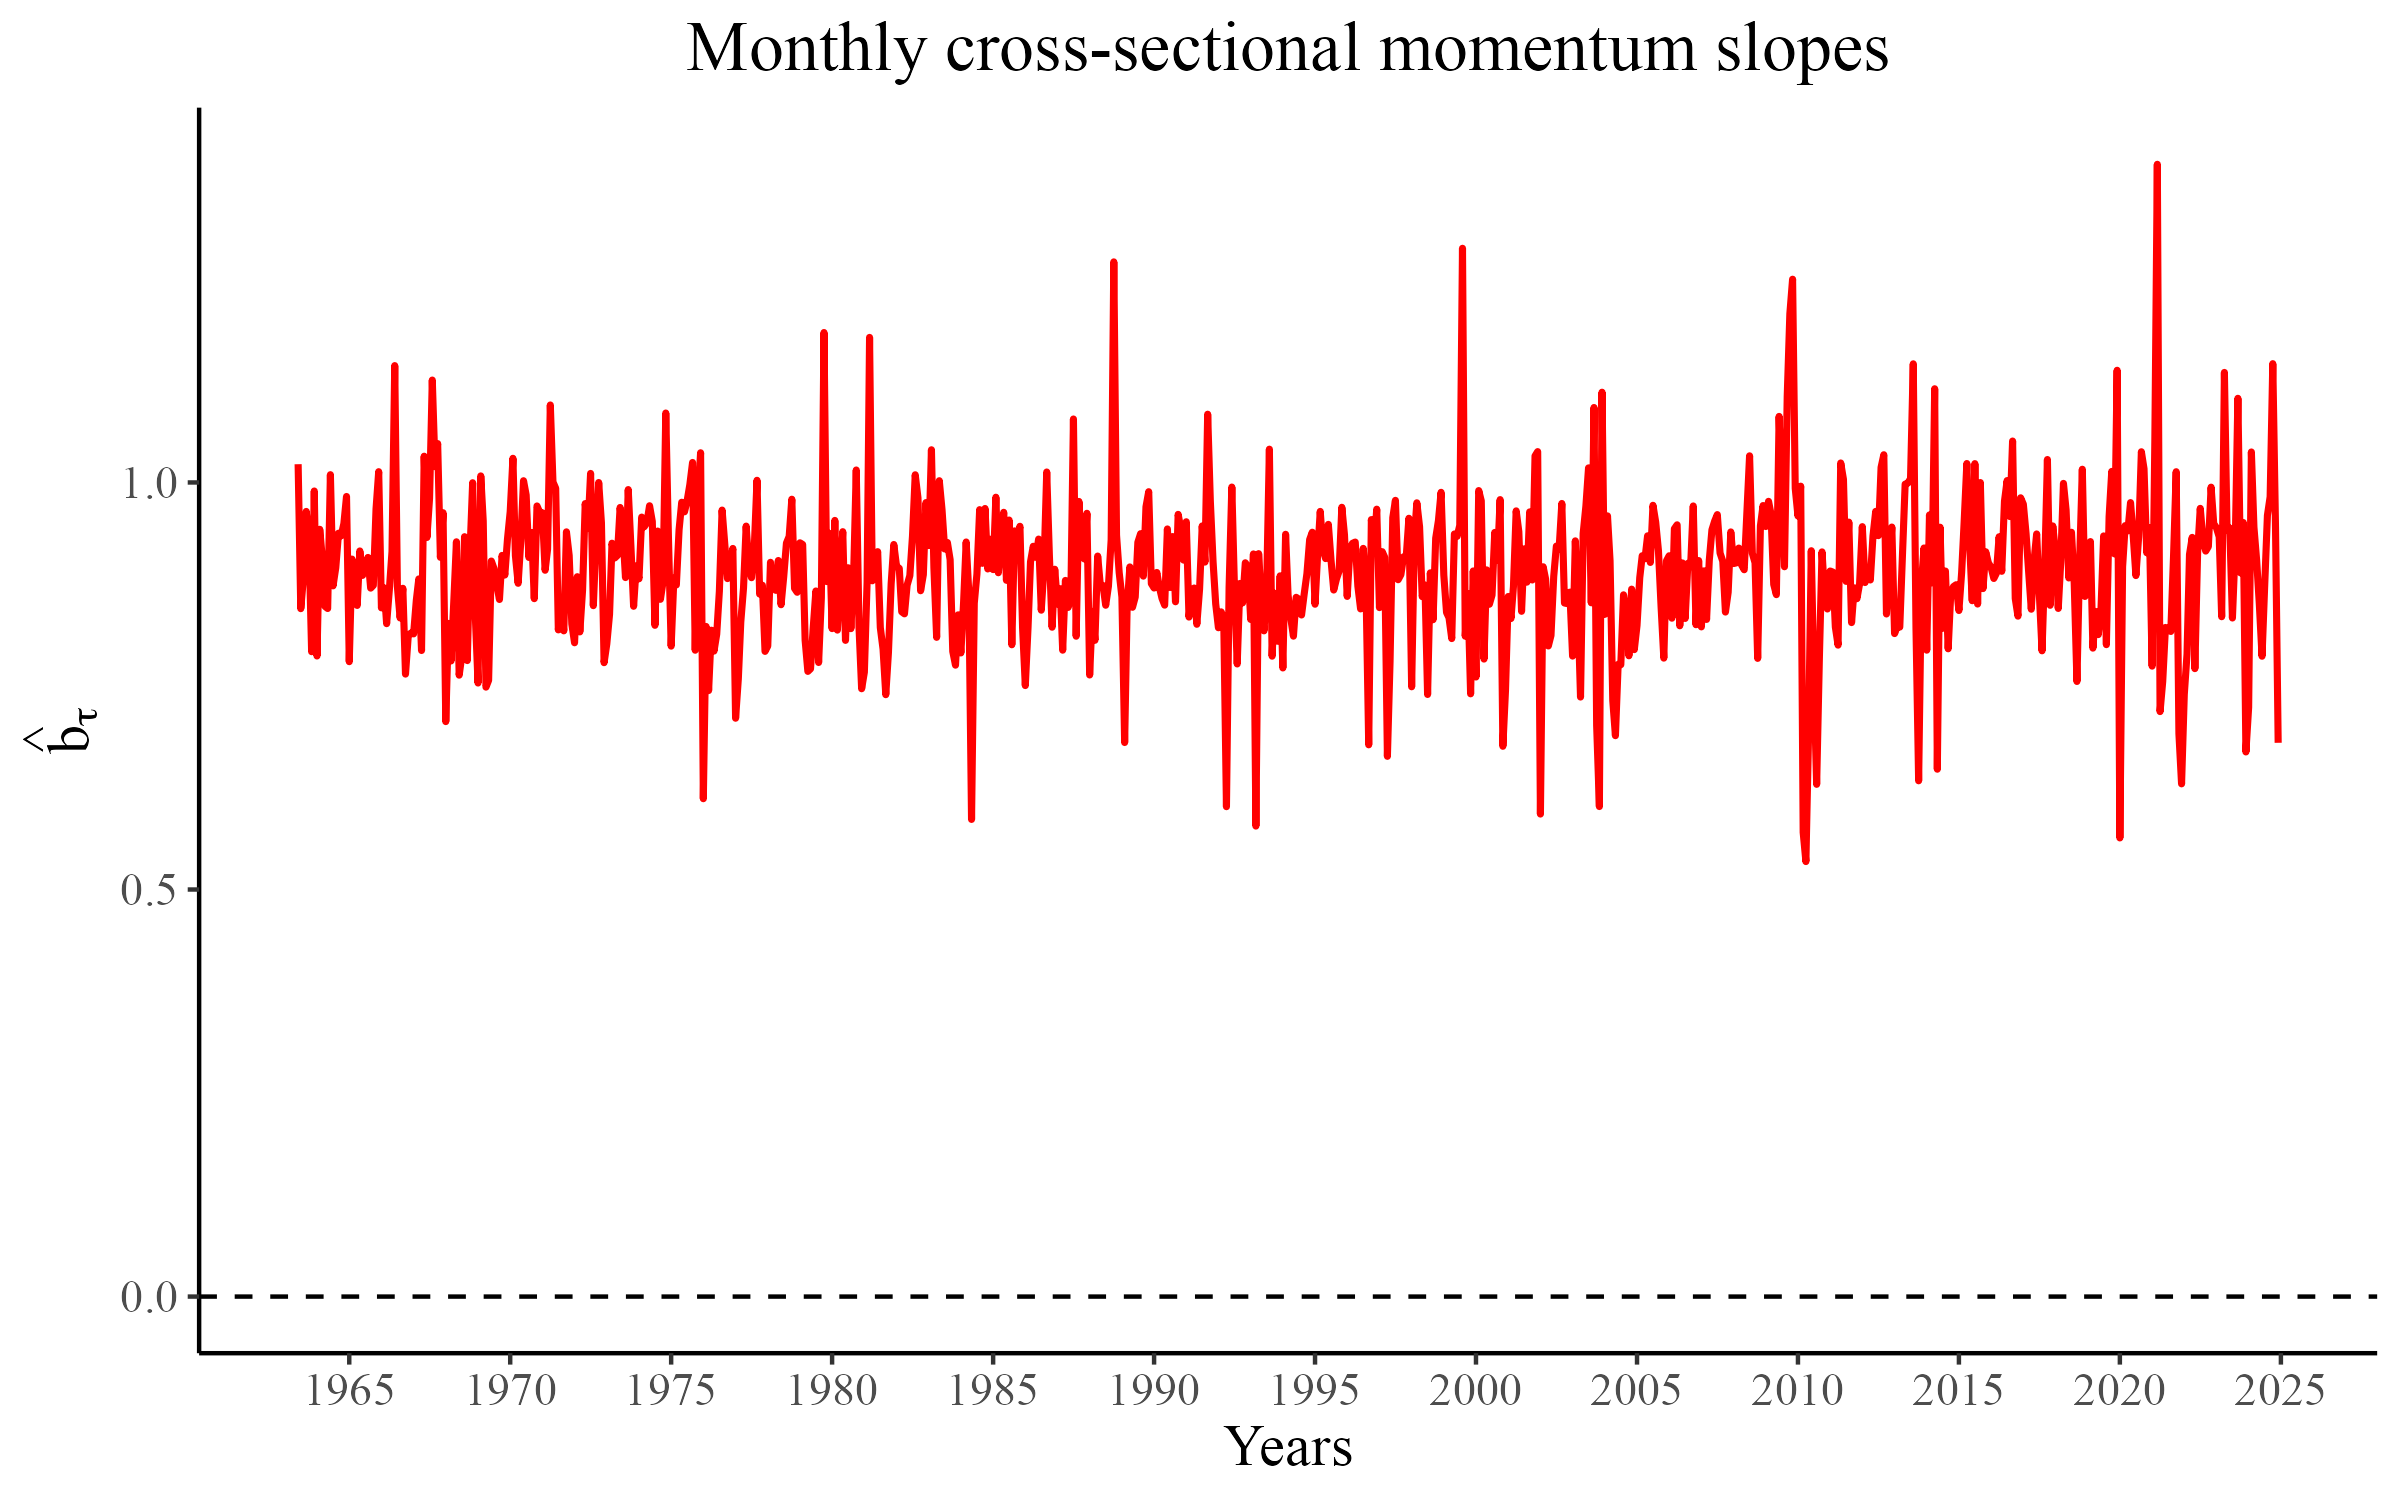
\includegraphics[width=0.75\textwidth]{figures/3a_slope.png}
    \label{fig:q10}
\end{figure}

\begin{figure}[H]
    \centering
    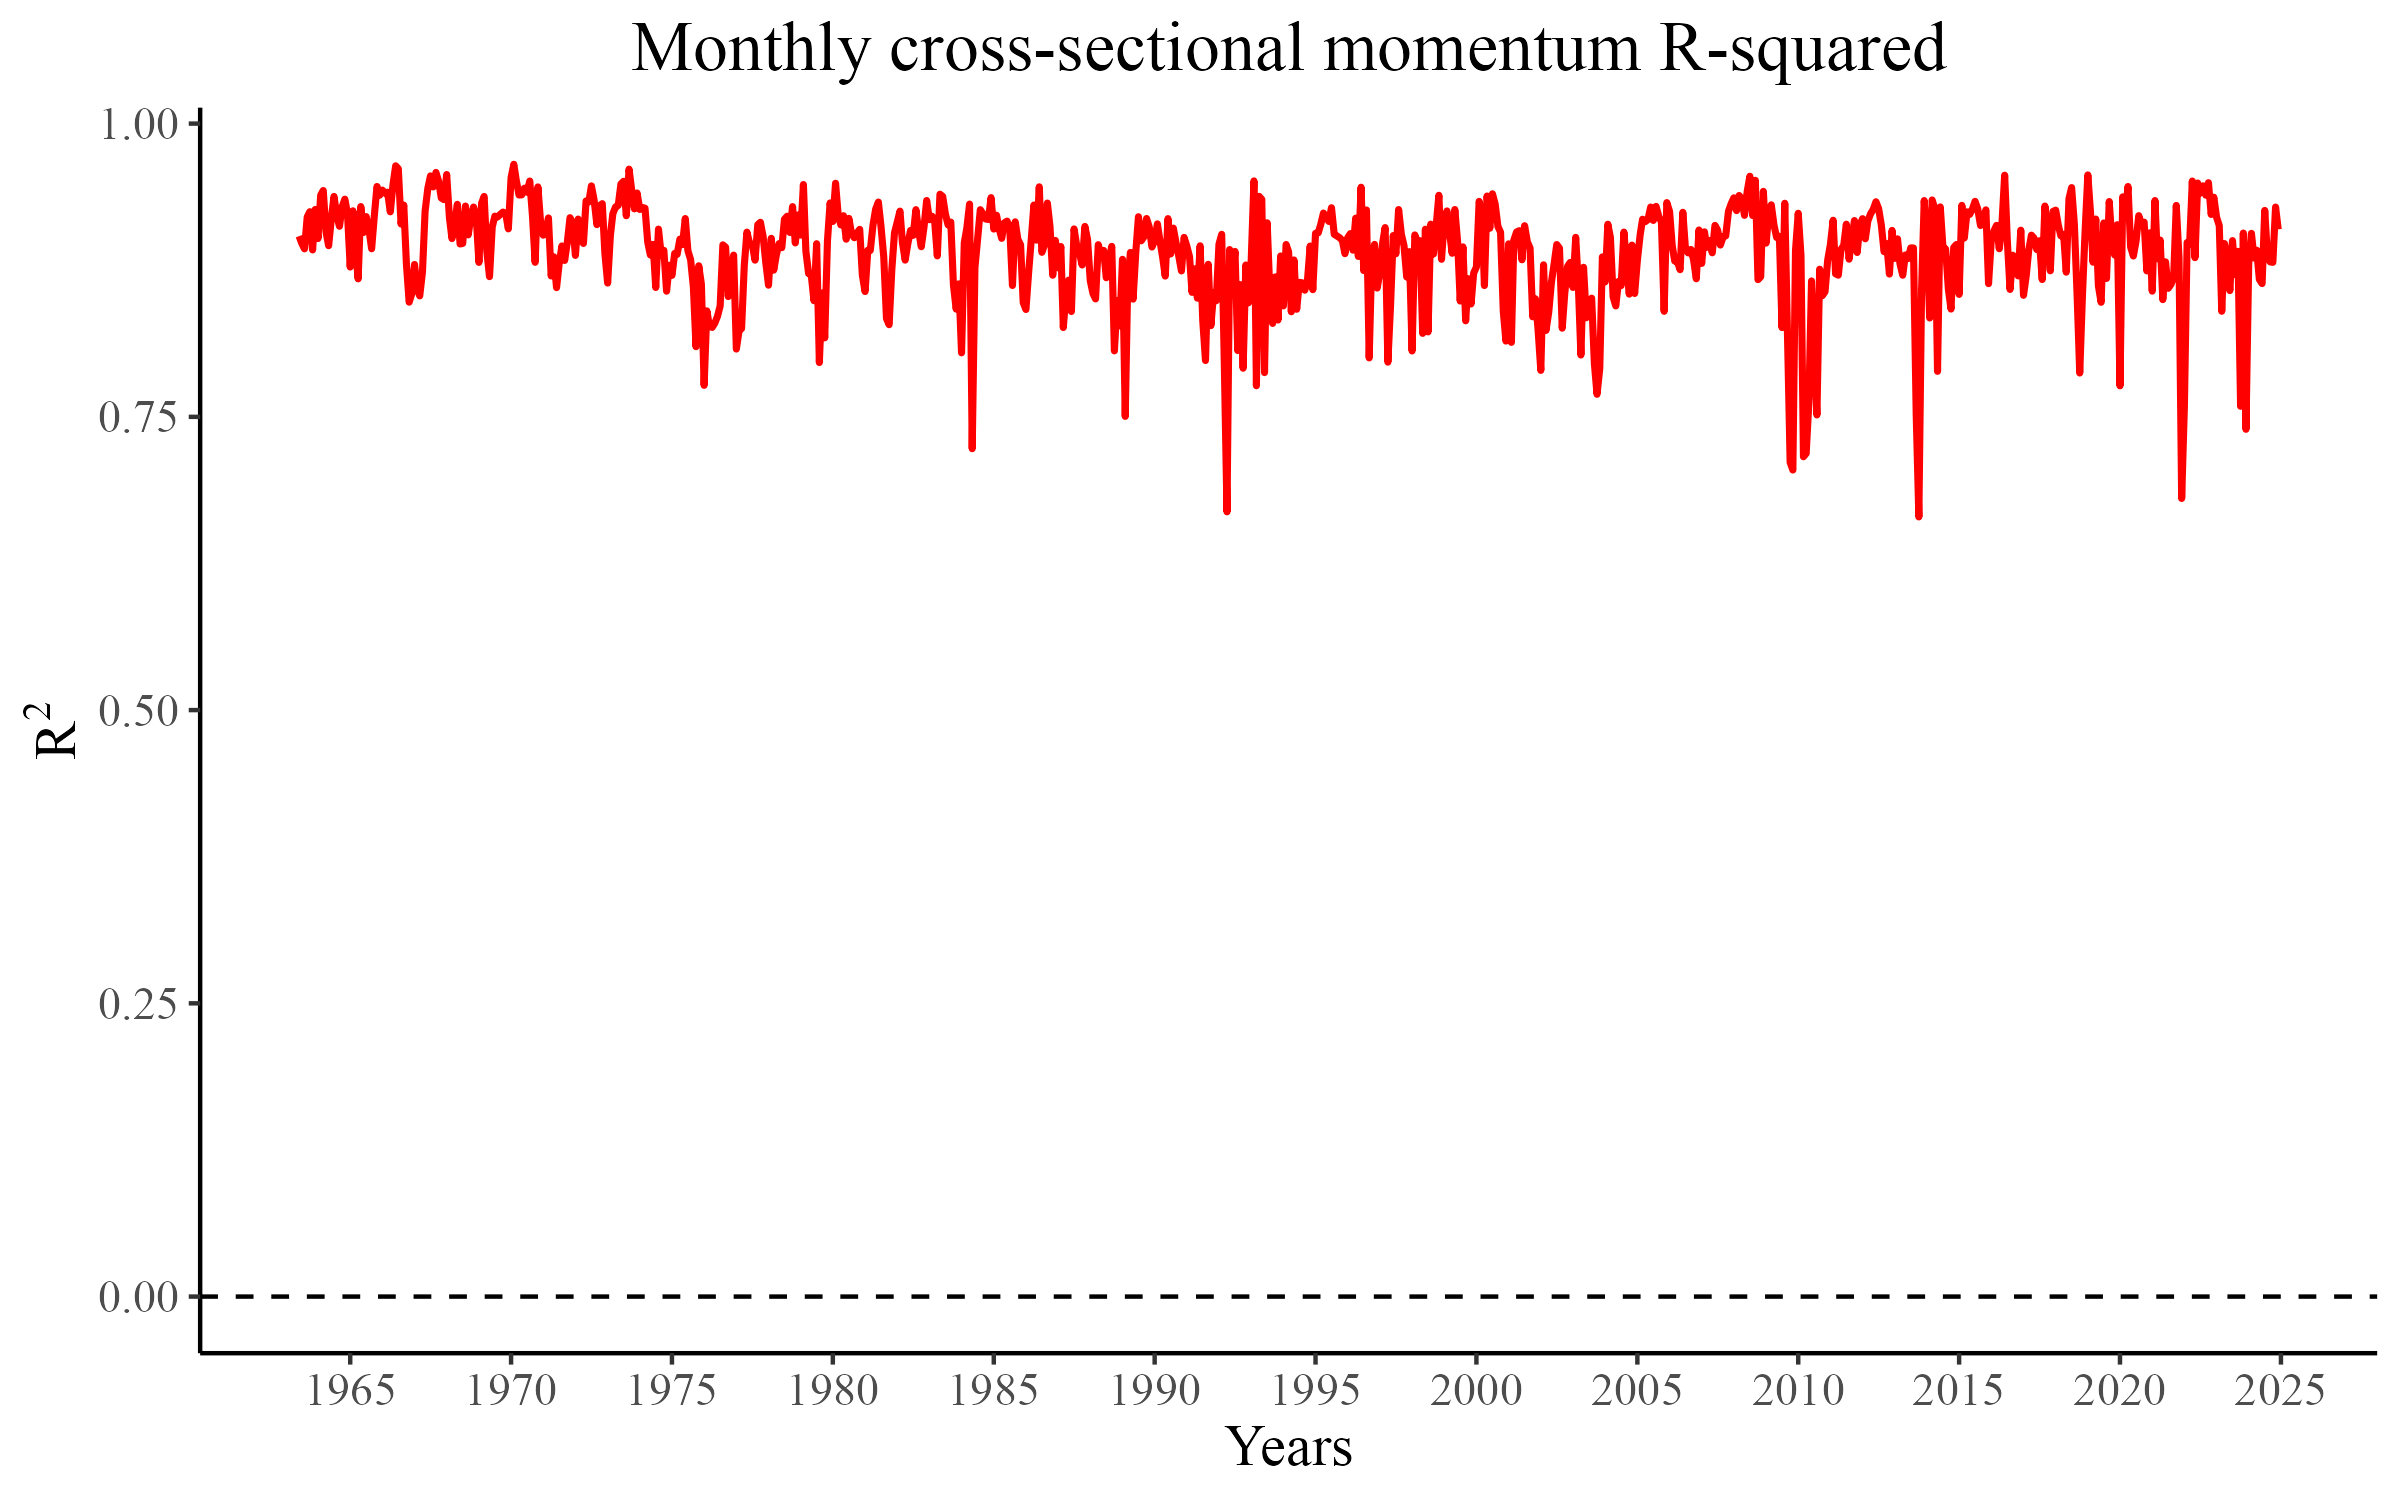
\includegraphics[width=0.75\textwidth]{figures/3a_Rsquared.png}
    \label{fig:q11}
\end{figure}

As observed in these plots, the intercepts and slopes bounced around 0 and 1 with $R^{2}$ close to 1, suggesting that the constructed $BM$ closely tracks $BM\_CZ$. 

\subsection*{3 (b)} 
Using the Fundamental Annual under the CRSP/COMPUSTAT Merged dataset, I computed the annual book equity $BE = SE + TXDITC - BVPS$ following the instructions in the footnote. I then imposed the backfilling bias restriction requiring that firms need at least 2 years of data, in addition to the requirement of $BE > 0$ and $CURCD = USD$. I also verified that there is a unique observation for each $GVKEY$ and $FYEAR$ pair using the standard Compustat Annual filters ($LINKTYPE = LC$ or $LU$ and $LINKPRIM = P$ or $C$ with preferences for the former). Then, using the cleaned CRSP dataset, I calculated the December market equity in millions as:
\[
ME_{j,\tau} = \frac{|PRC_{j, \tau}| * SHROUT_{j, \tau}}{1000}
\]
Then, I linked these 2 datasets on $PERMNO$ and $YYYYMM$ and constructed the June book-to-market signal $BM$ in the fiscal year t using $BE$ and December $ME$ in the fiscal year t-1 as follows: 
\[
    BM_{j,t} = \frac{BE_{j,t-1}}{ME_{j,t-1}}
\]
I kept the constructed June $BM$ signal fixed from June of year t through May of year t+1 as the assigned monthly $BM$. After inspecting the unit levels of $BM$ and $BM\_CZ$, I ran a cross-sectional regression of $BM\_CZ$ on monthly $BM$ for each month $\tau$ as a validation test and retrieved the following variables: 
\[
    BM\_CZ_{j, \tau} = a_\tau + b_\tau * BM_{j, \tau} + e_{j, \tau}
\]

\begin{figure}[H]
    \centering
    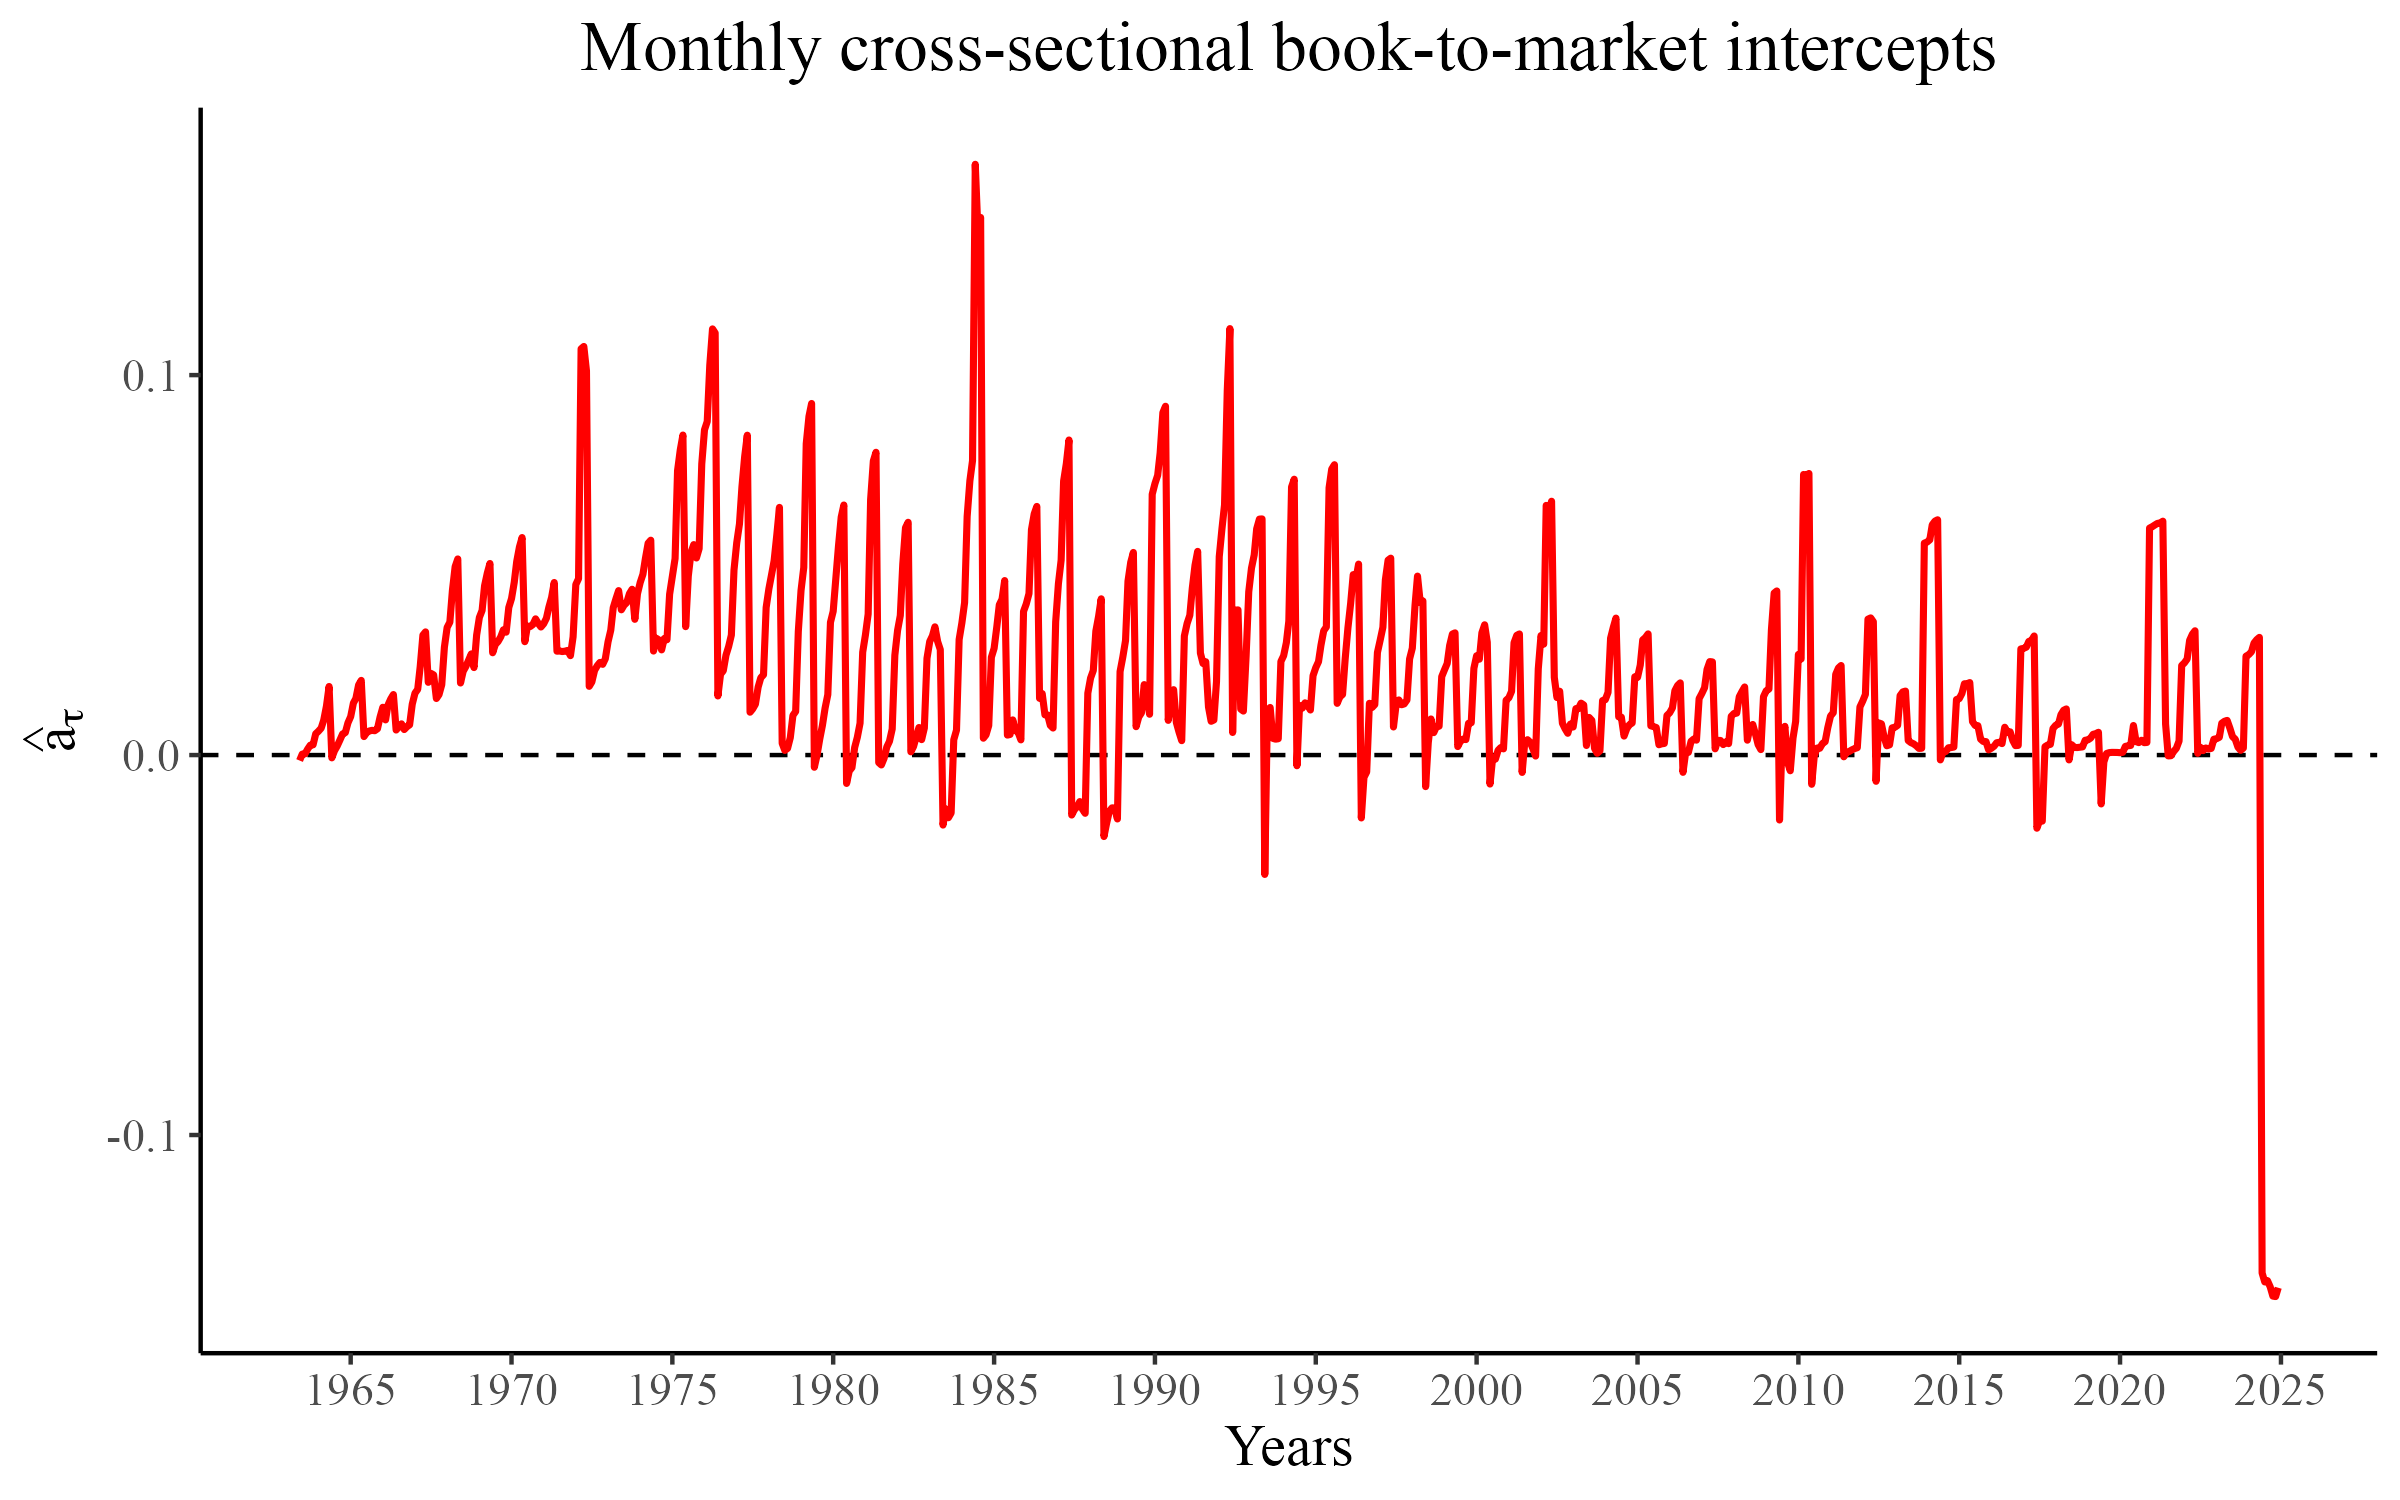
\includegraphics[width=0.75\textwidth]{figures/3b_intercept.png}
    \label{fig:q13}
\end{figure}

\begin{figure}[H]
    \centering
    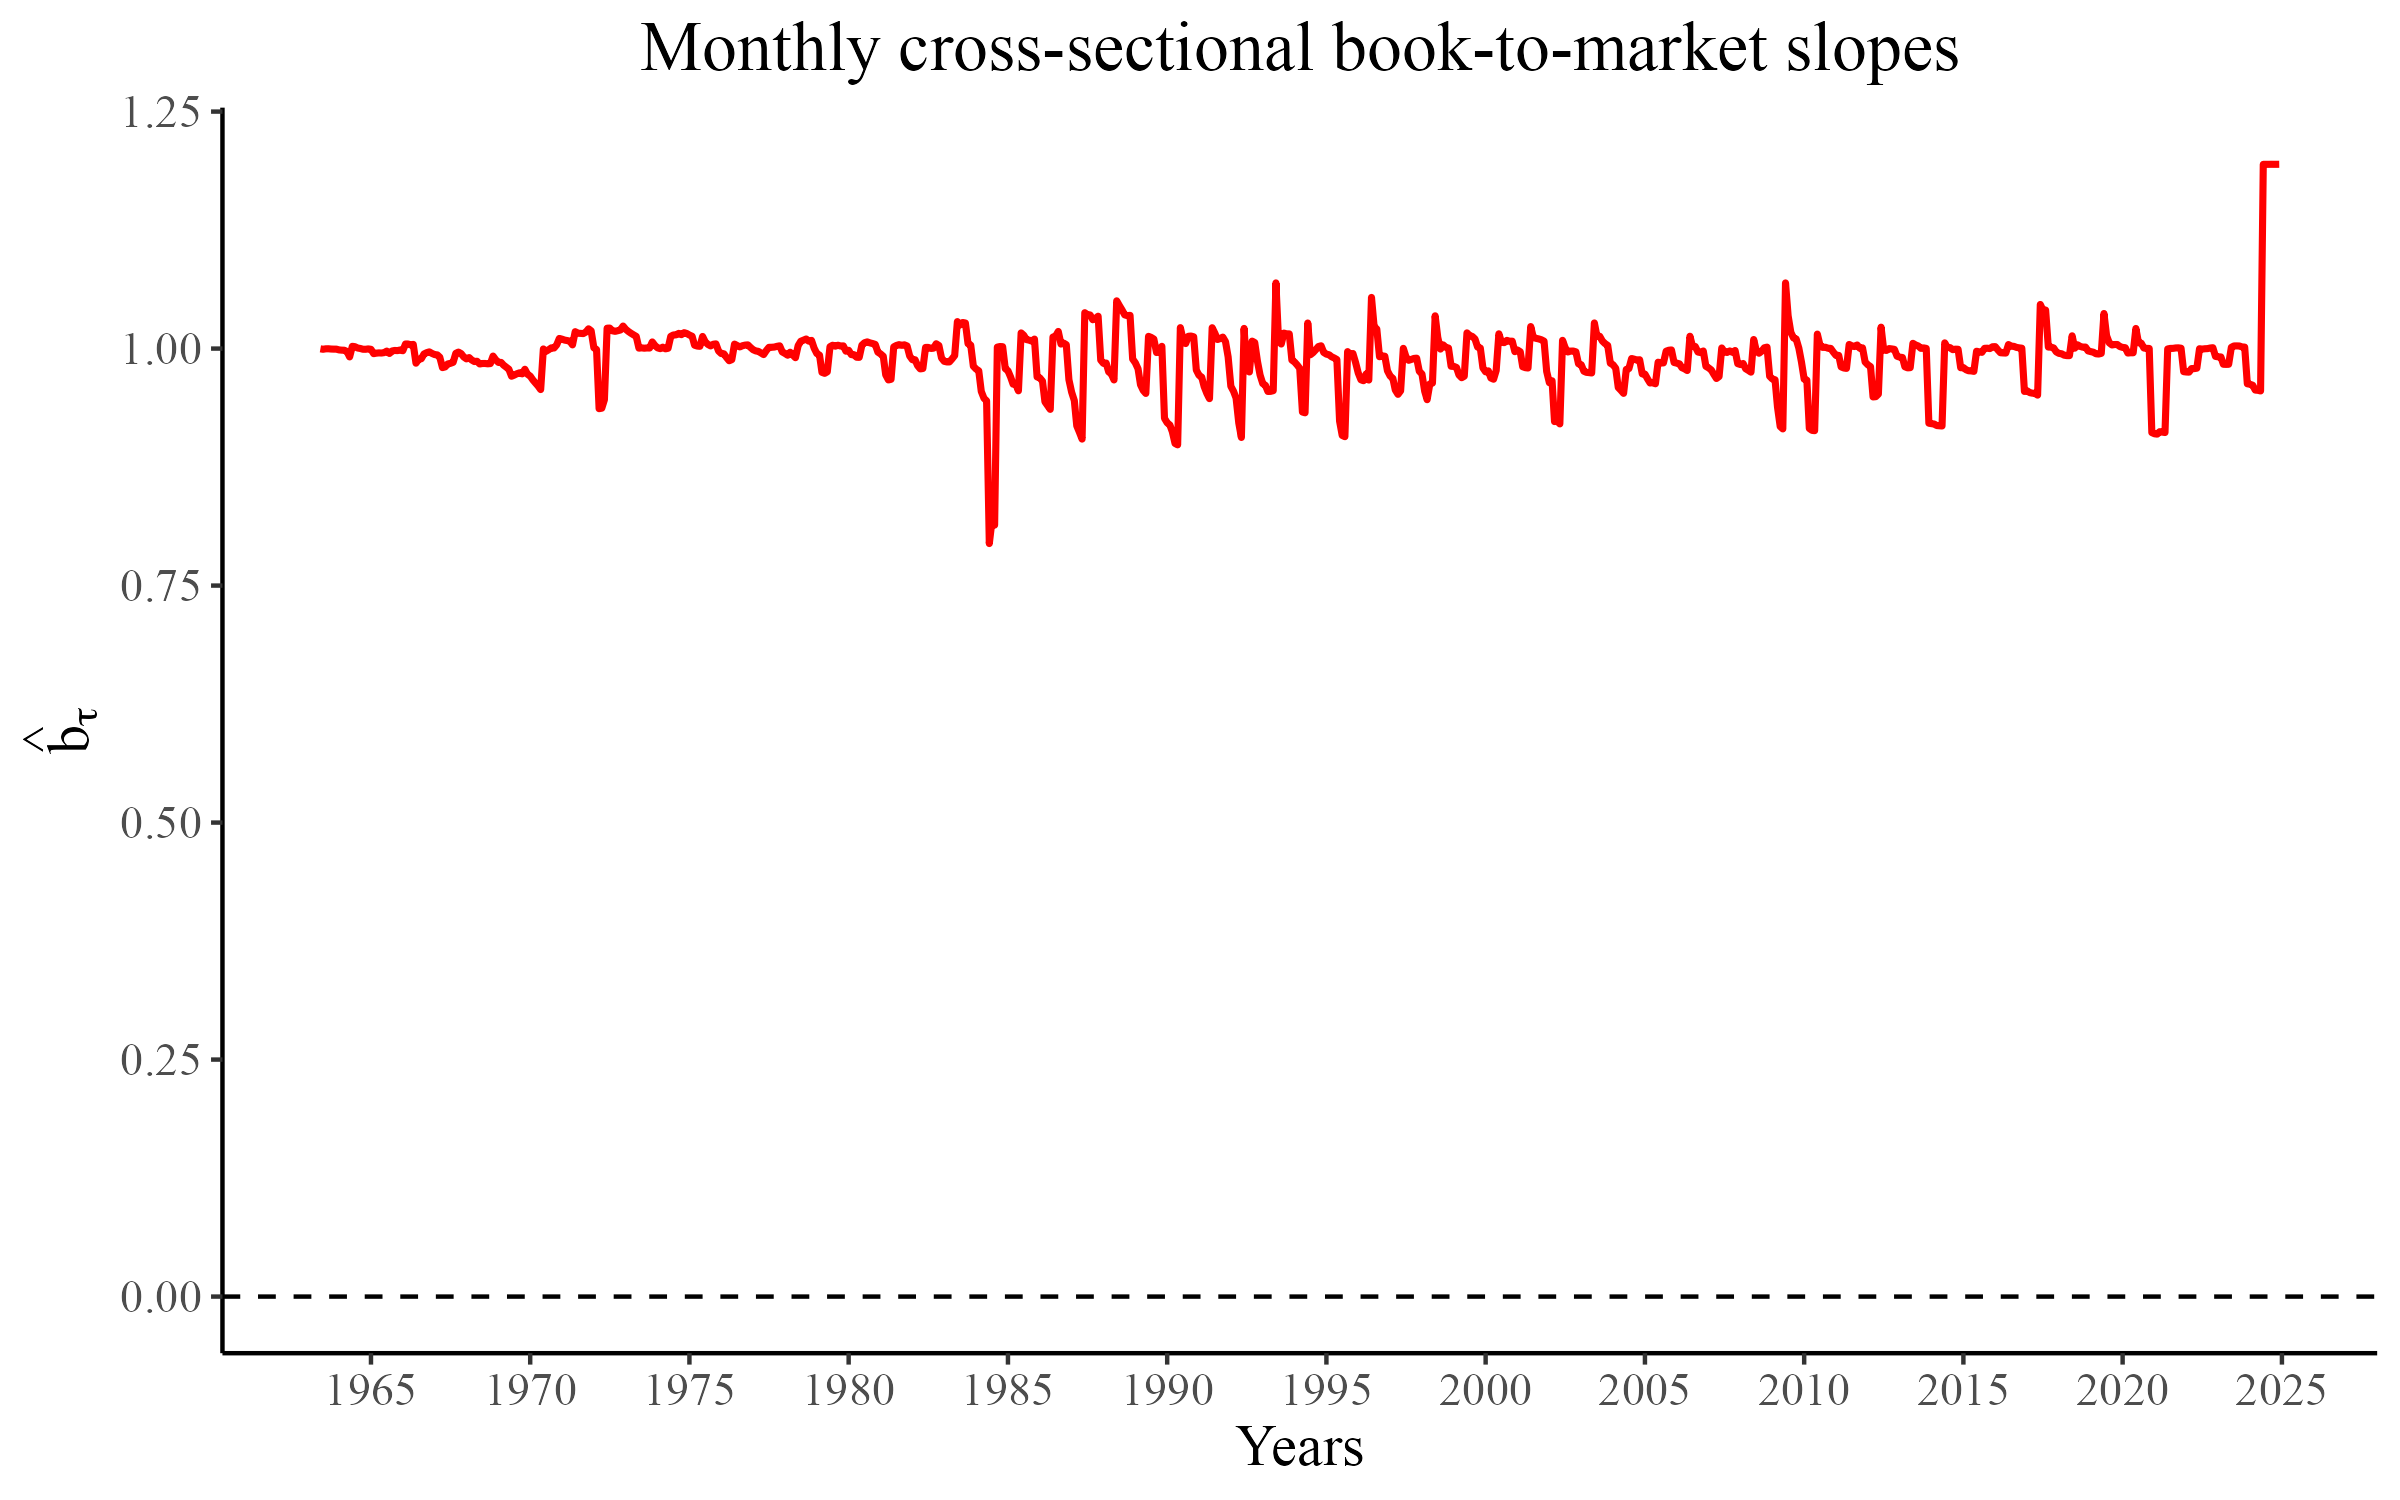
\includegraphics[width=0.75\textwidth]{figures/3b_slope.png}
    \label{fig:q14}
\end{figure}

\begin{figure}[H]
    \centering
    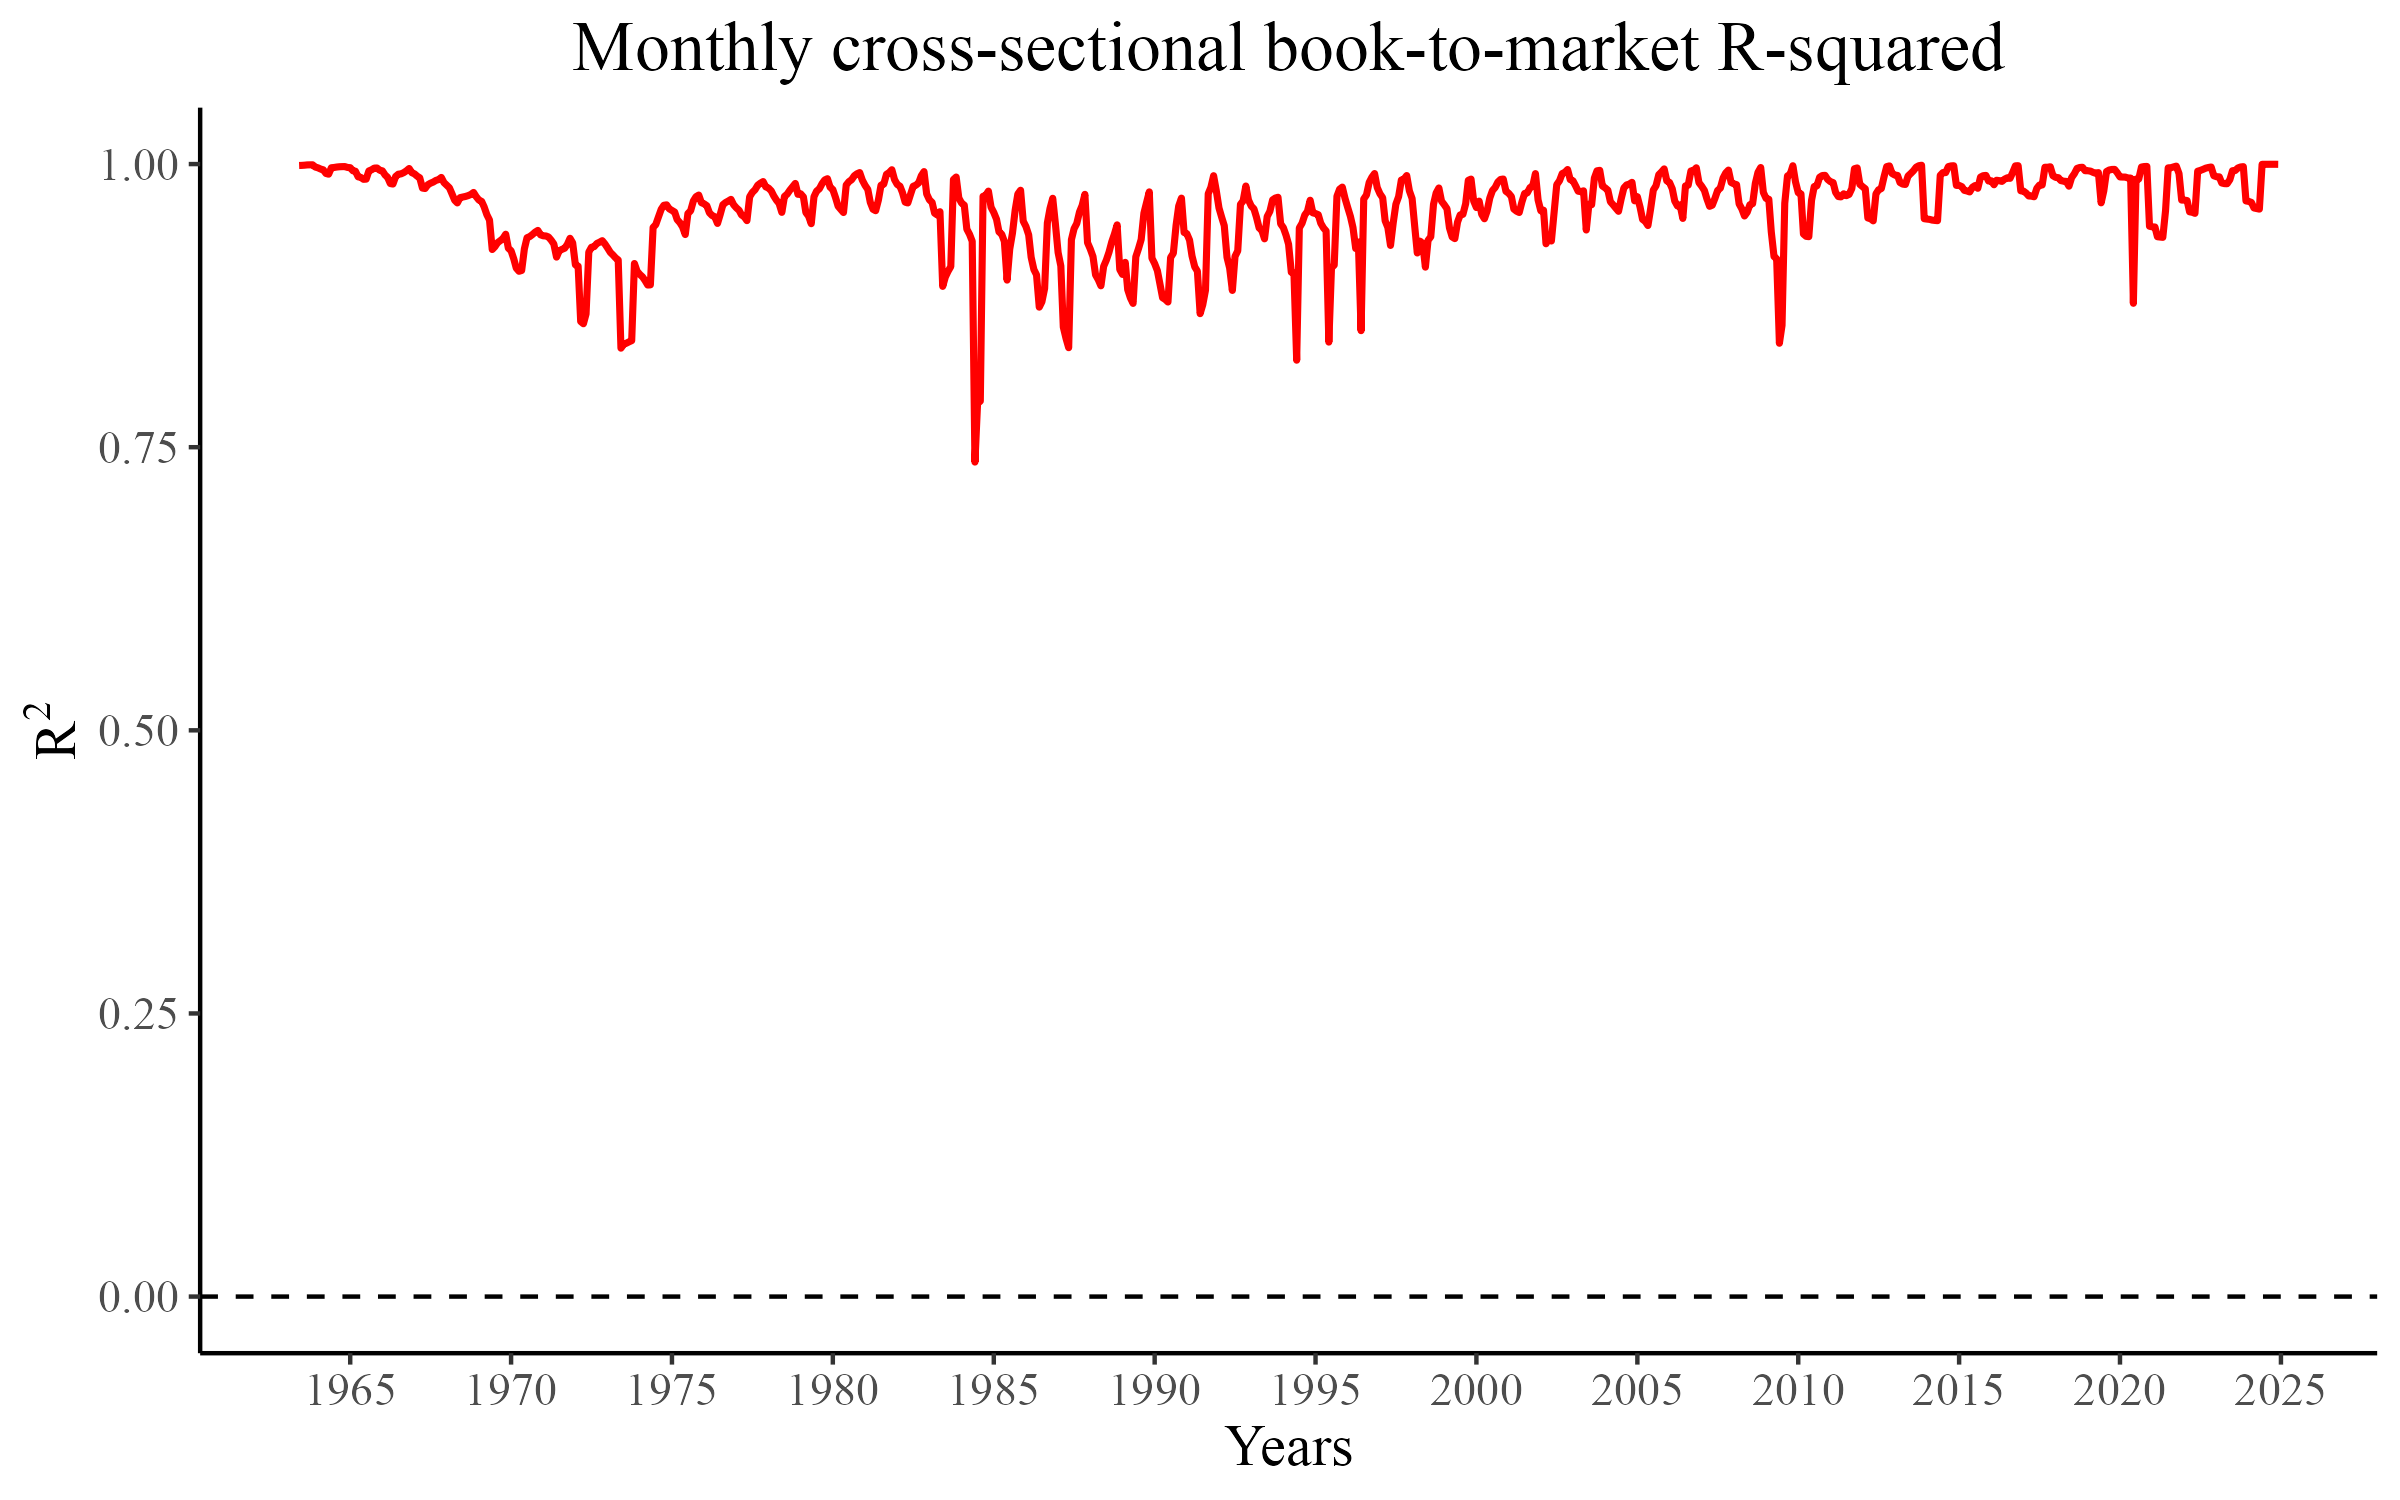
\includegraphics[width=0.75\textwidth]{figures/3b_Rsquared.png}
    \label{fig:q15}
\end{figure}

Except for an outlier observed in 2025, the constructed June $BM$ variable closely tracks $BM\_CZ$ with $R^2$ close to 1.
\subsection*{3 (c)} 
Following the sorting methods, I constructed 5 types of decile portfolios for each Chen-Zimmermann signal and retrieved their average monthly excess returns as follows: 

\begin{figure}[H]
    \centering
    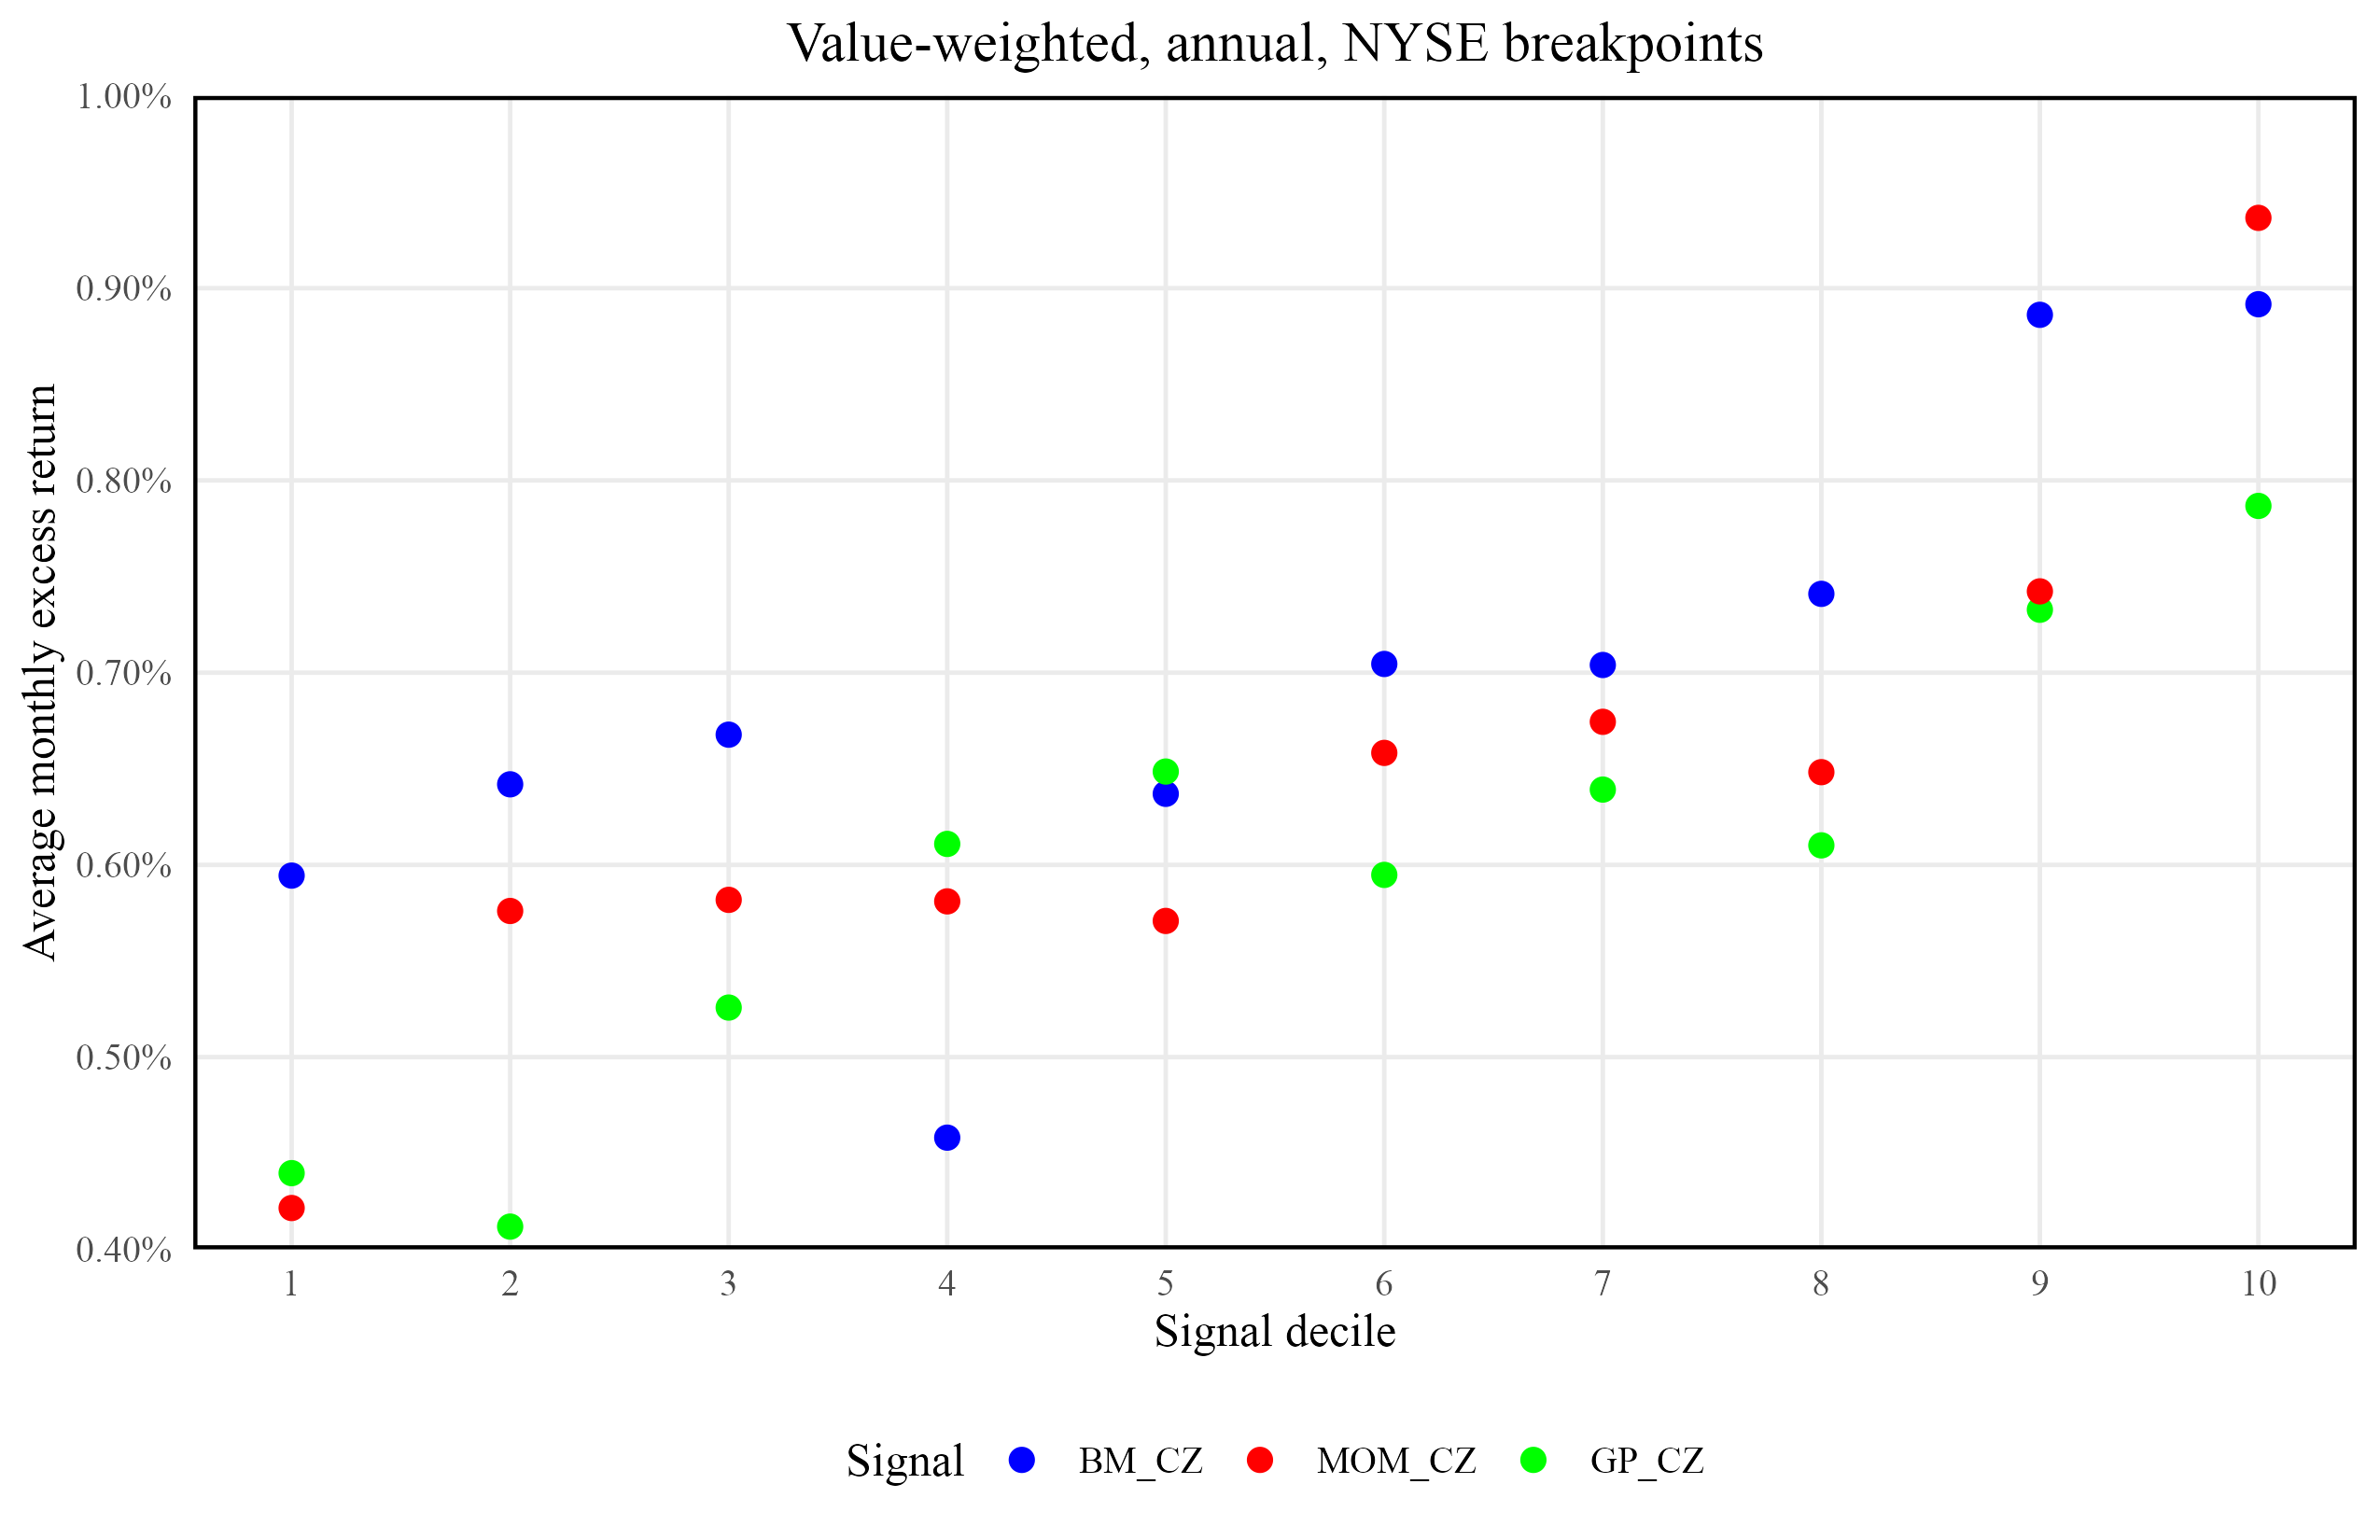
\includegraphics[width=0.70\textwidth]{figures/3c_i.png}
    \label{fig:q16}
\end{figure}

\begin{figure}[H]
    \centering
    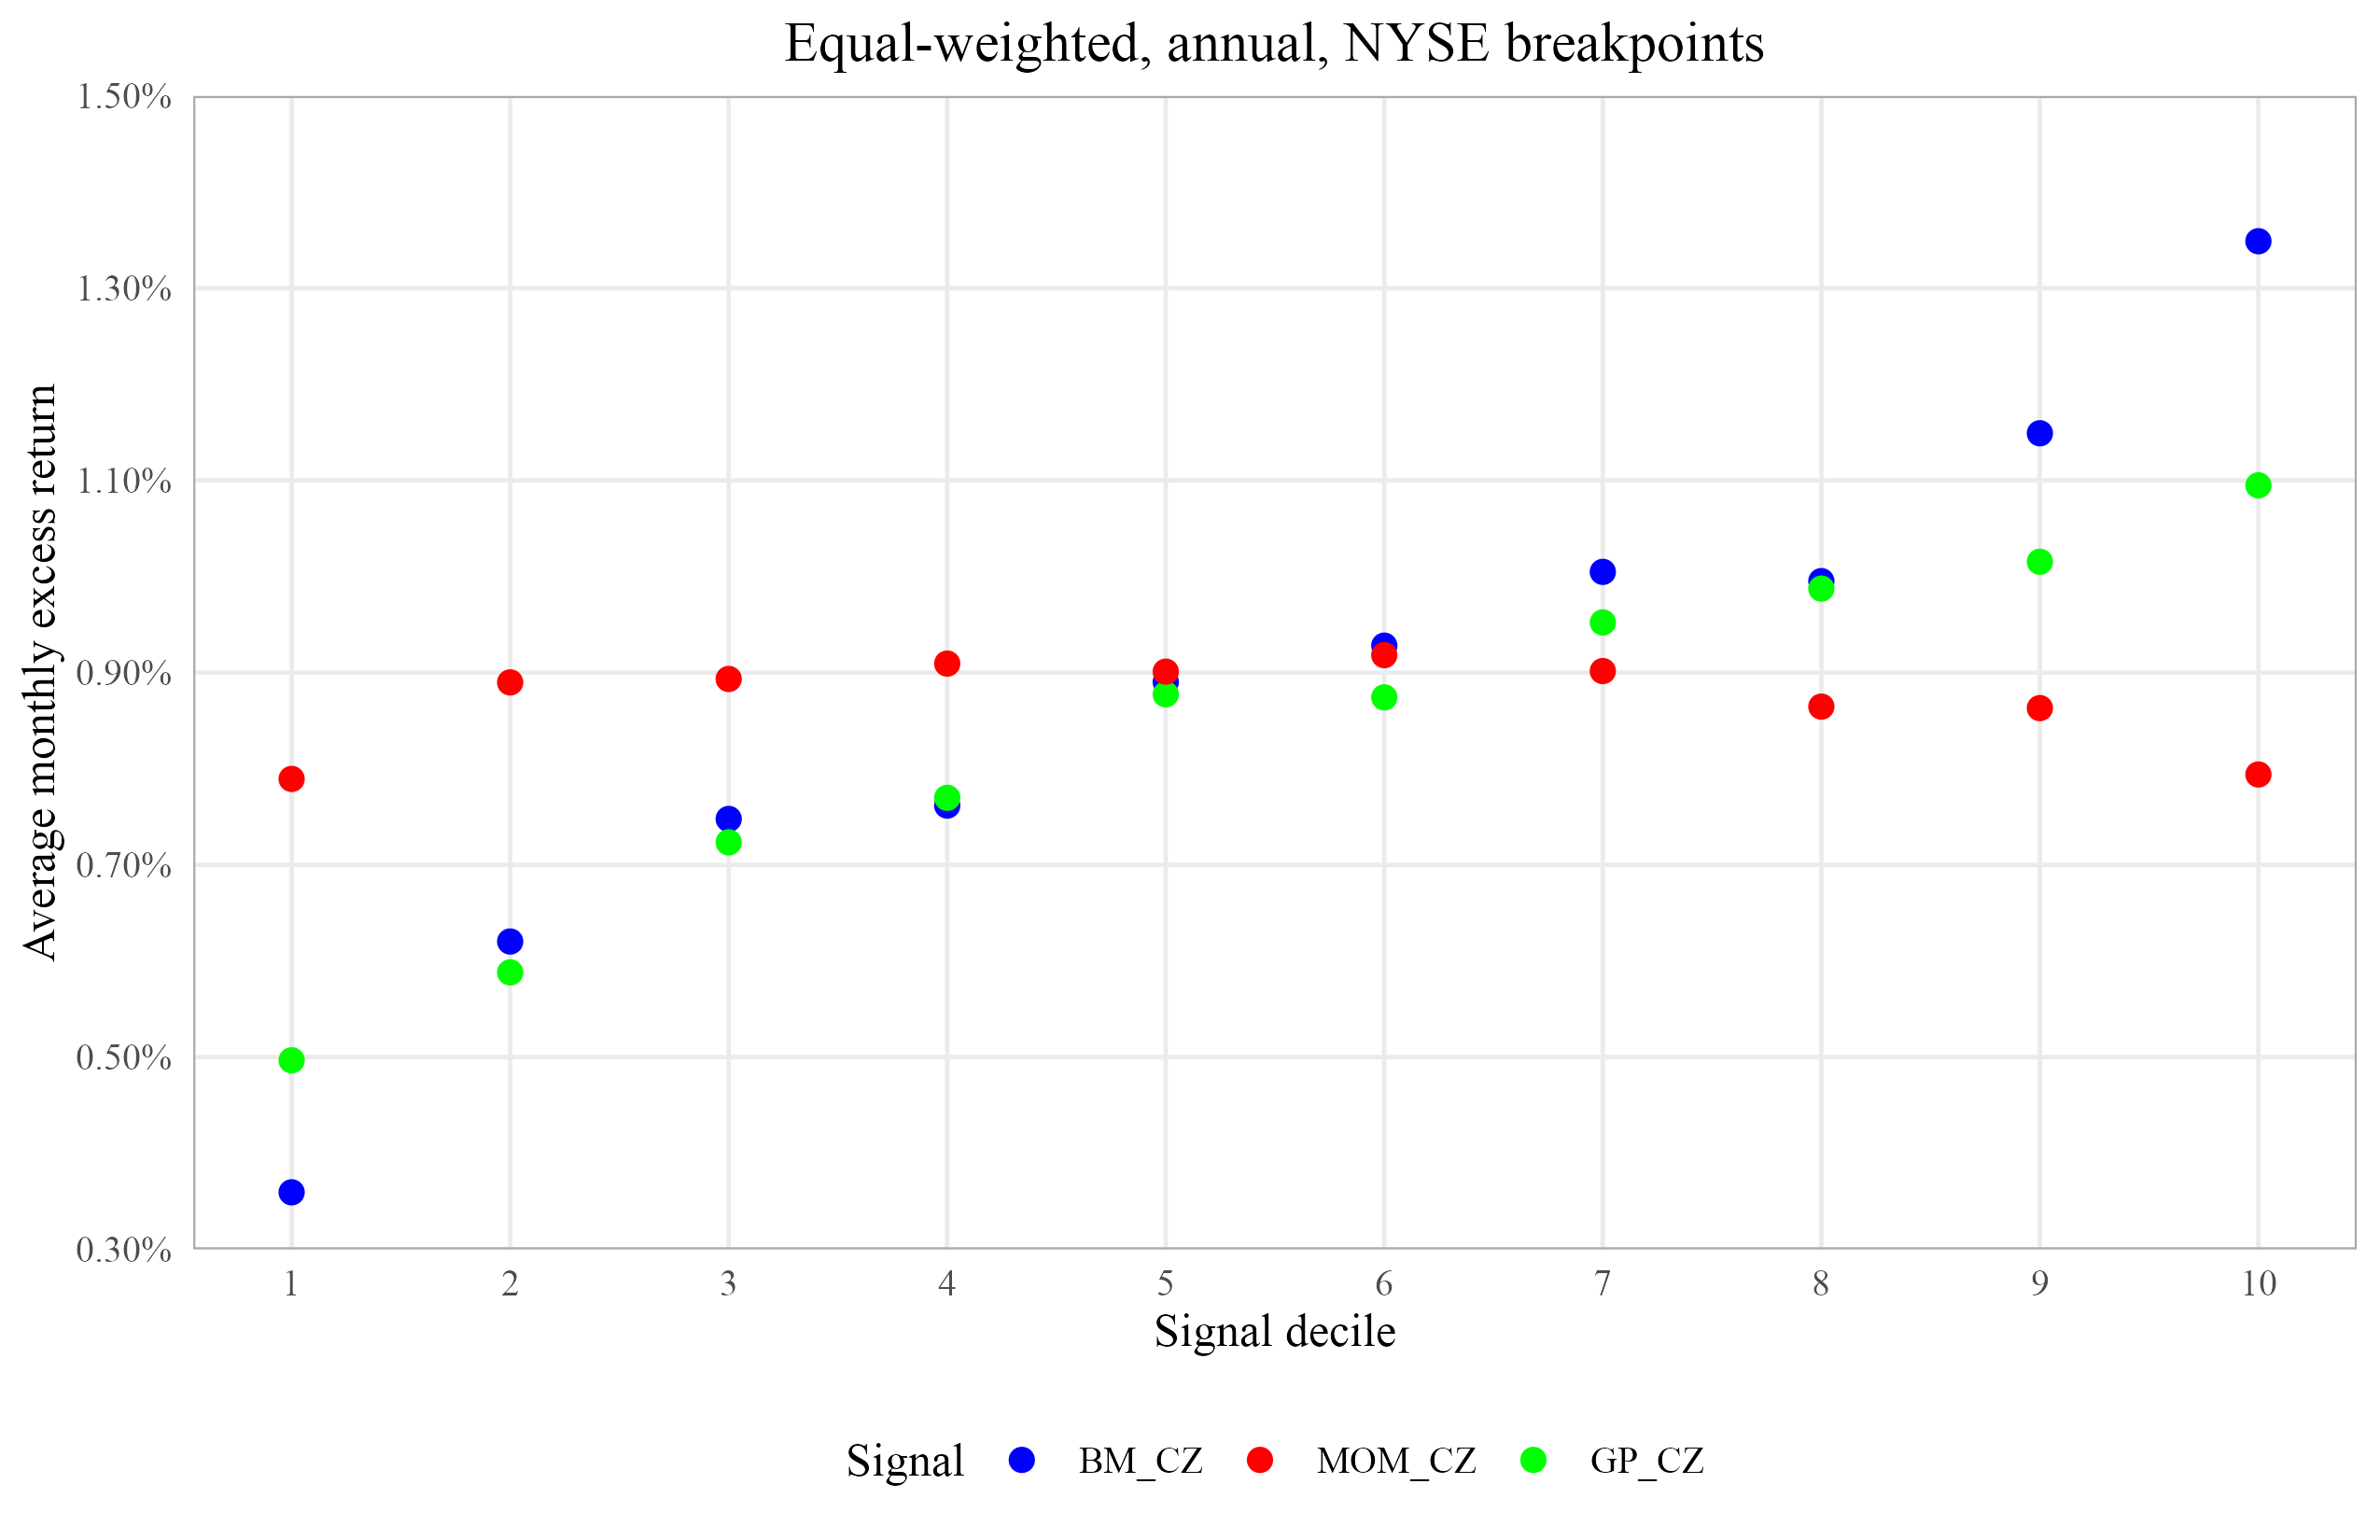
\includegraphics[width=0.70\textwidth]{figures/3c_ii.png}
    \label{fig:q17}
\end{figure}

\begin{figure}[H]
    \centering
    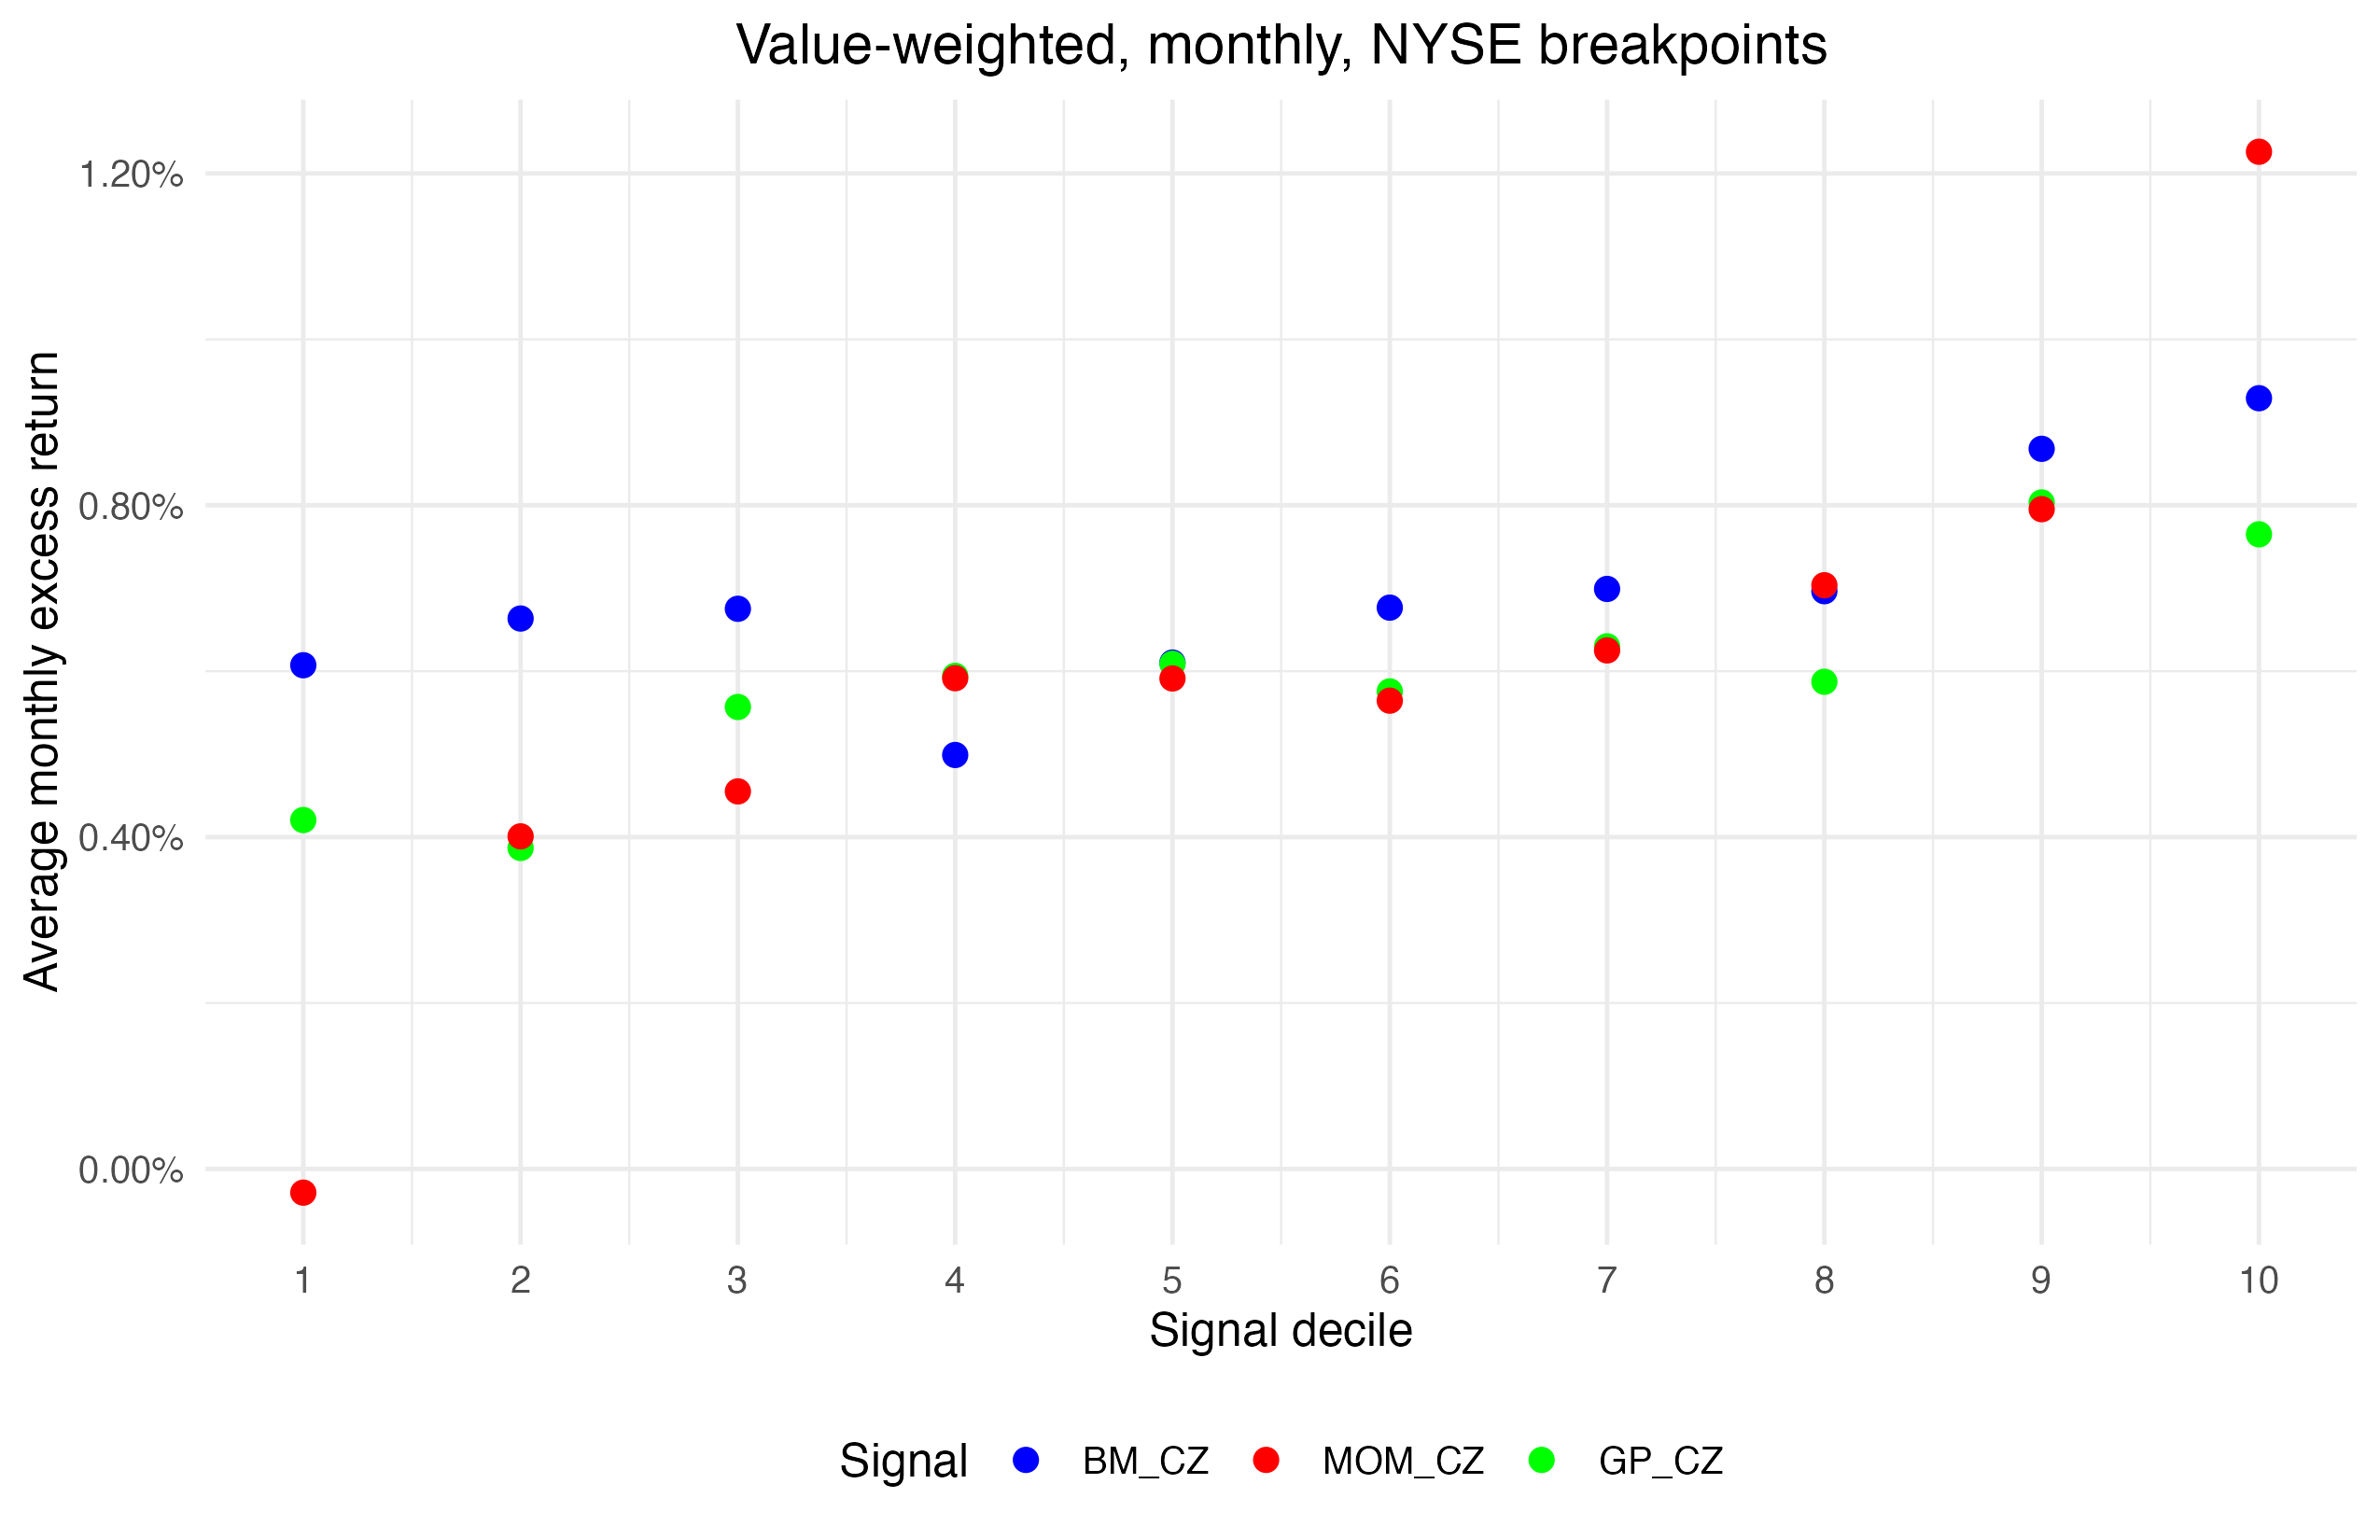
\includegraphics[width=0.70\textwidth]{figures/3c_iii.png}
    \label{fig:q18}
\end{figure}

\begin{figure}[H]
    \centering
    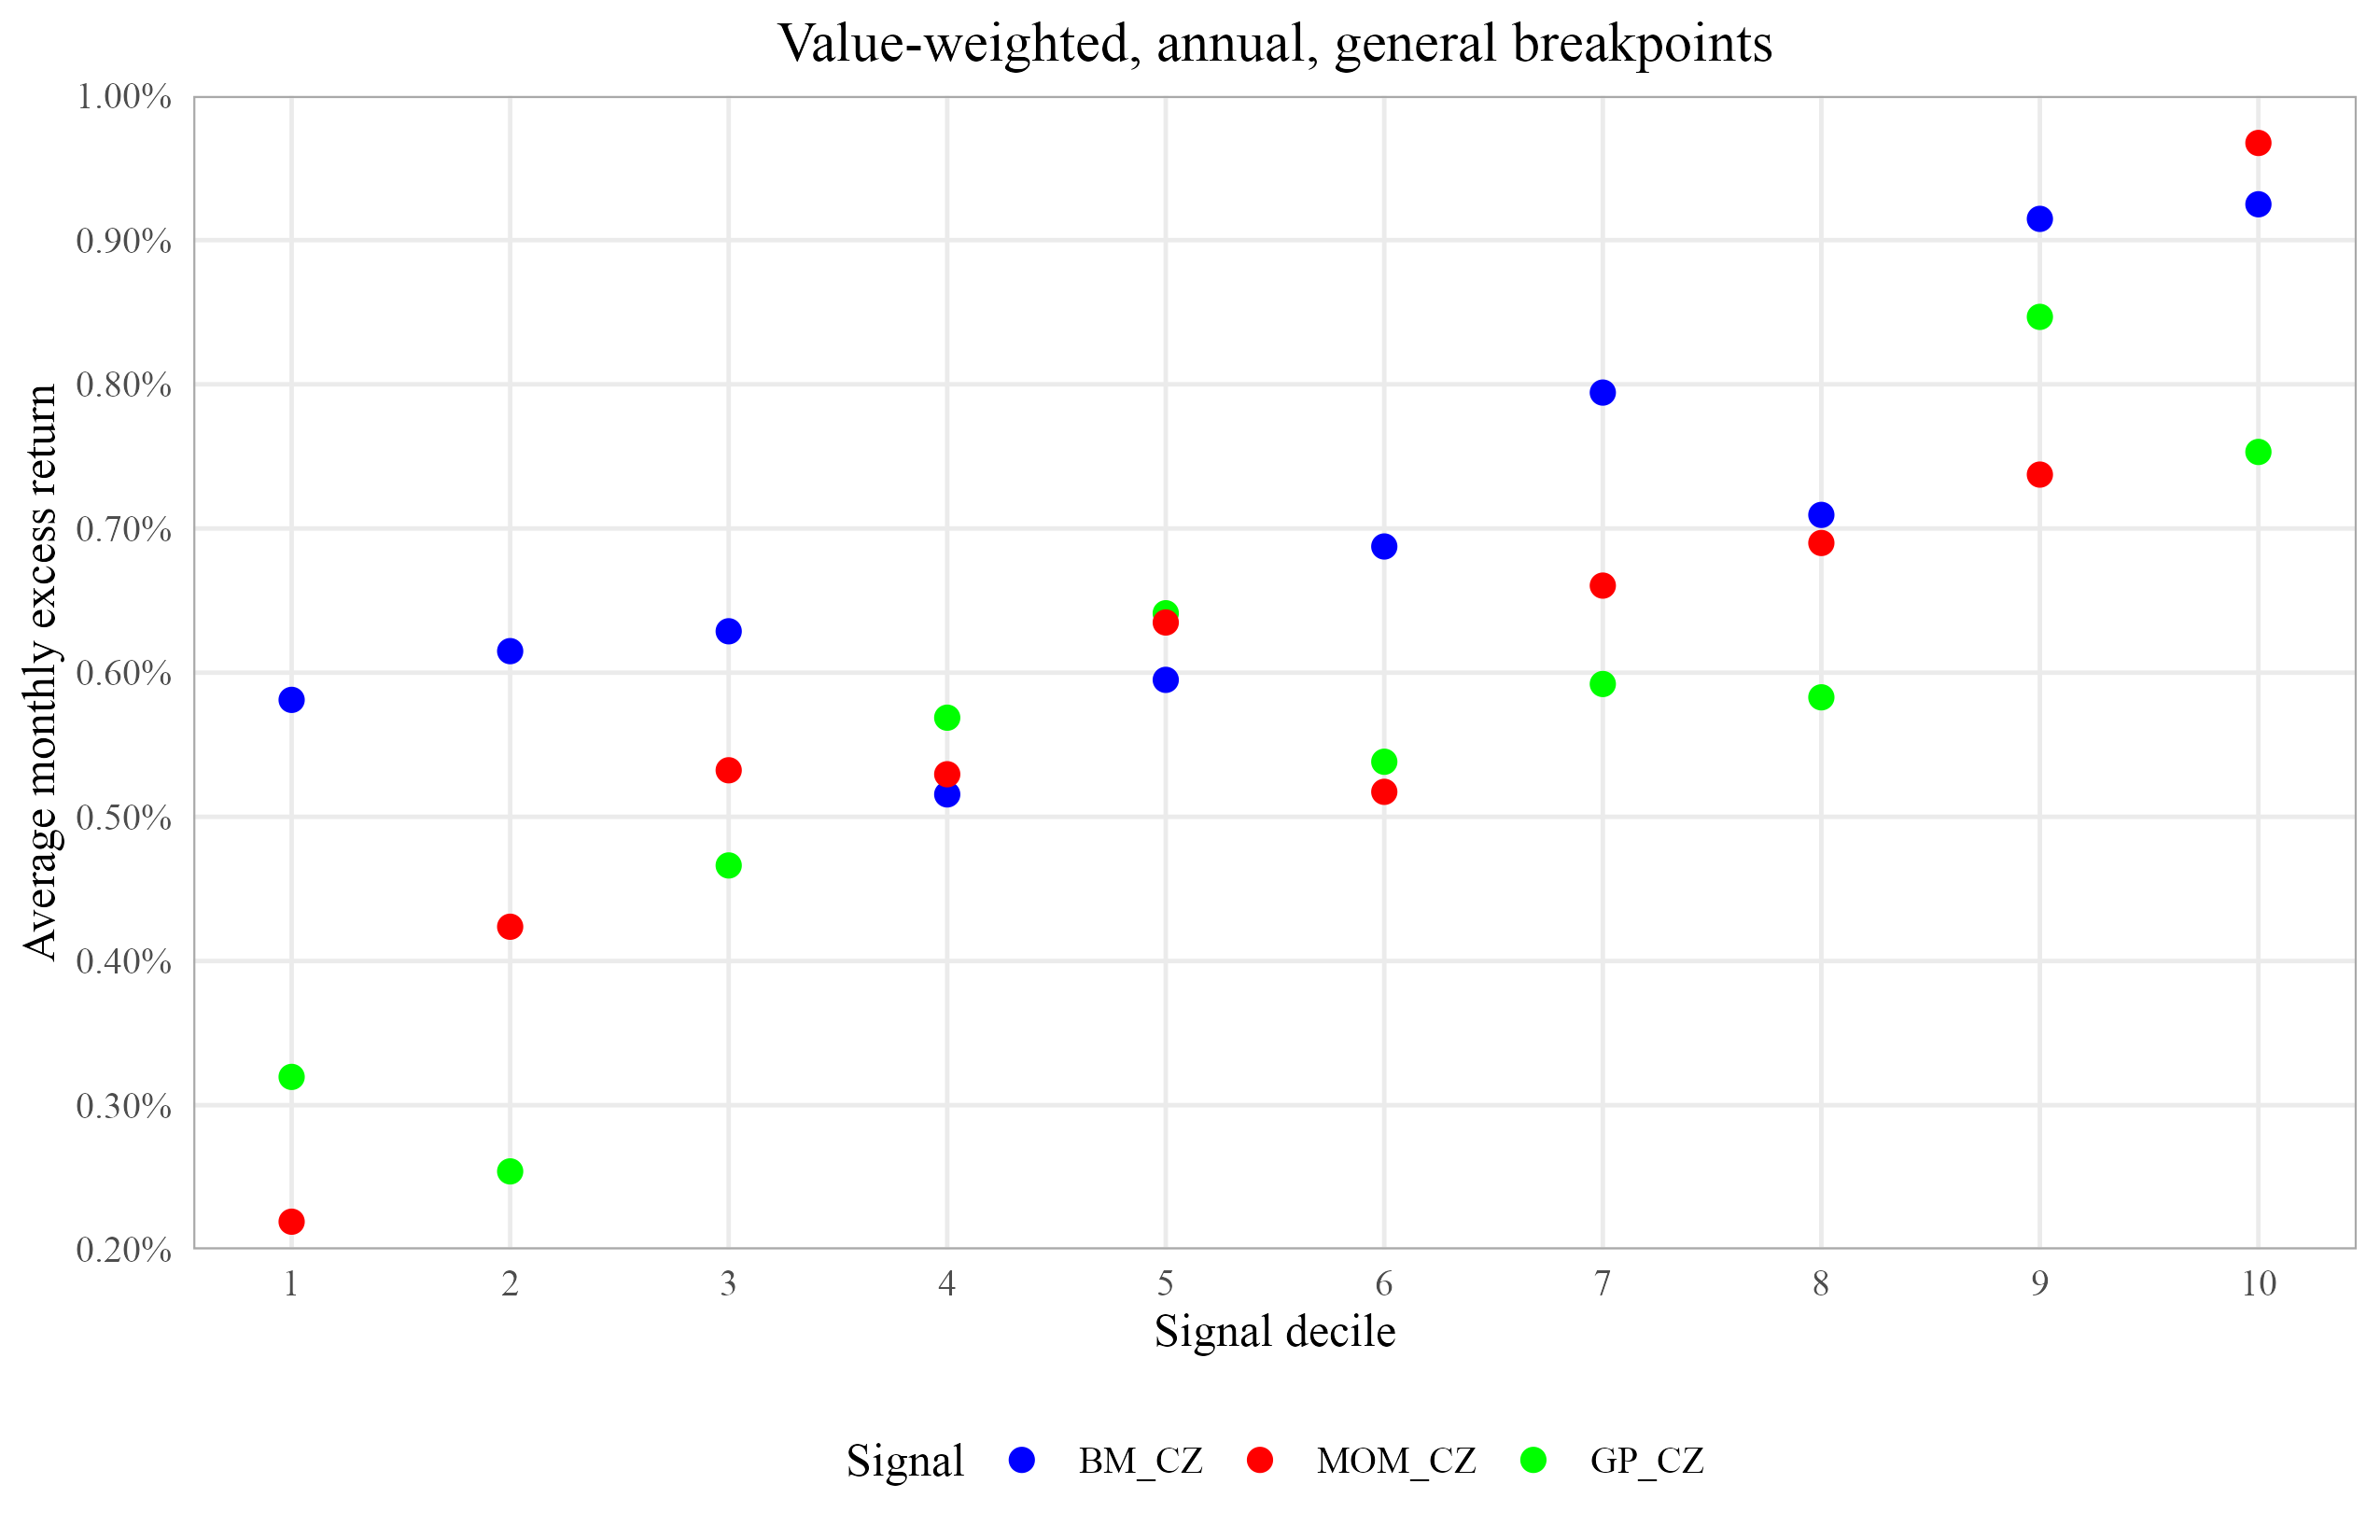
\includegraphics[width=0.70\textwidth]{figures/3c_iv.png}
    \label{fig:q19}
\end{figure}

\begin{figure}[H]
    \centering
    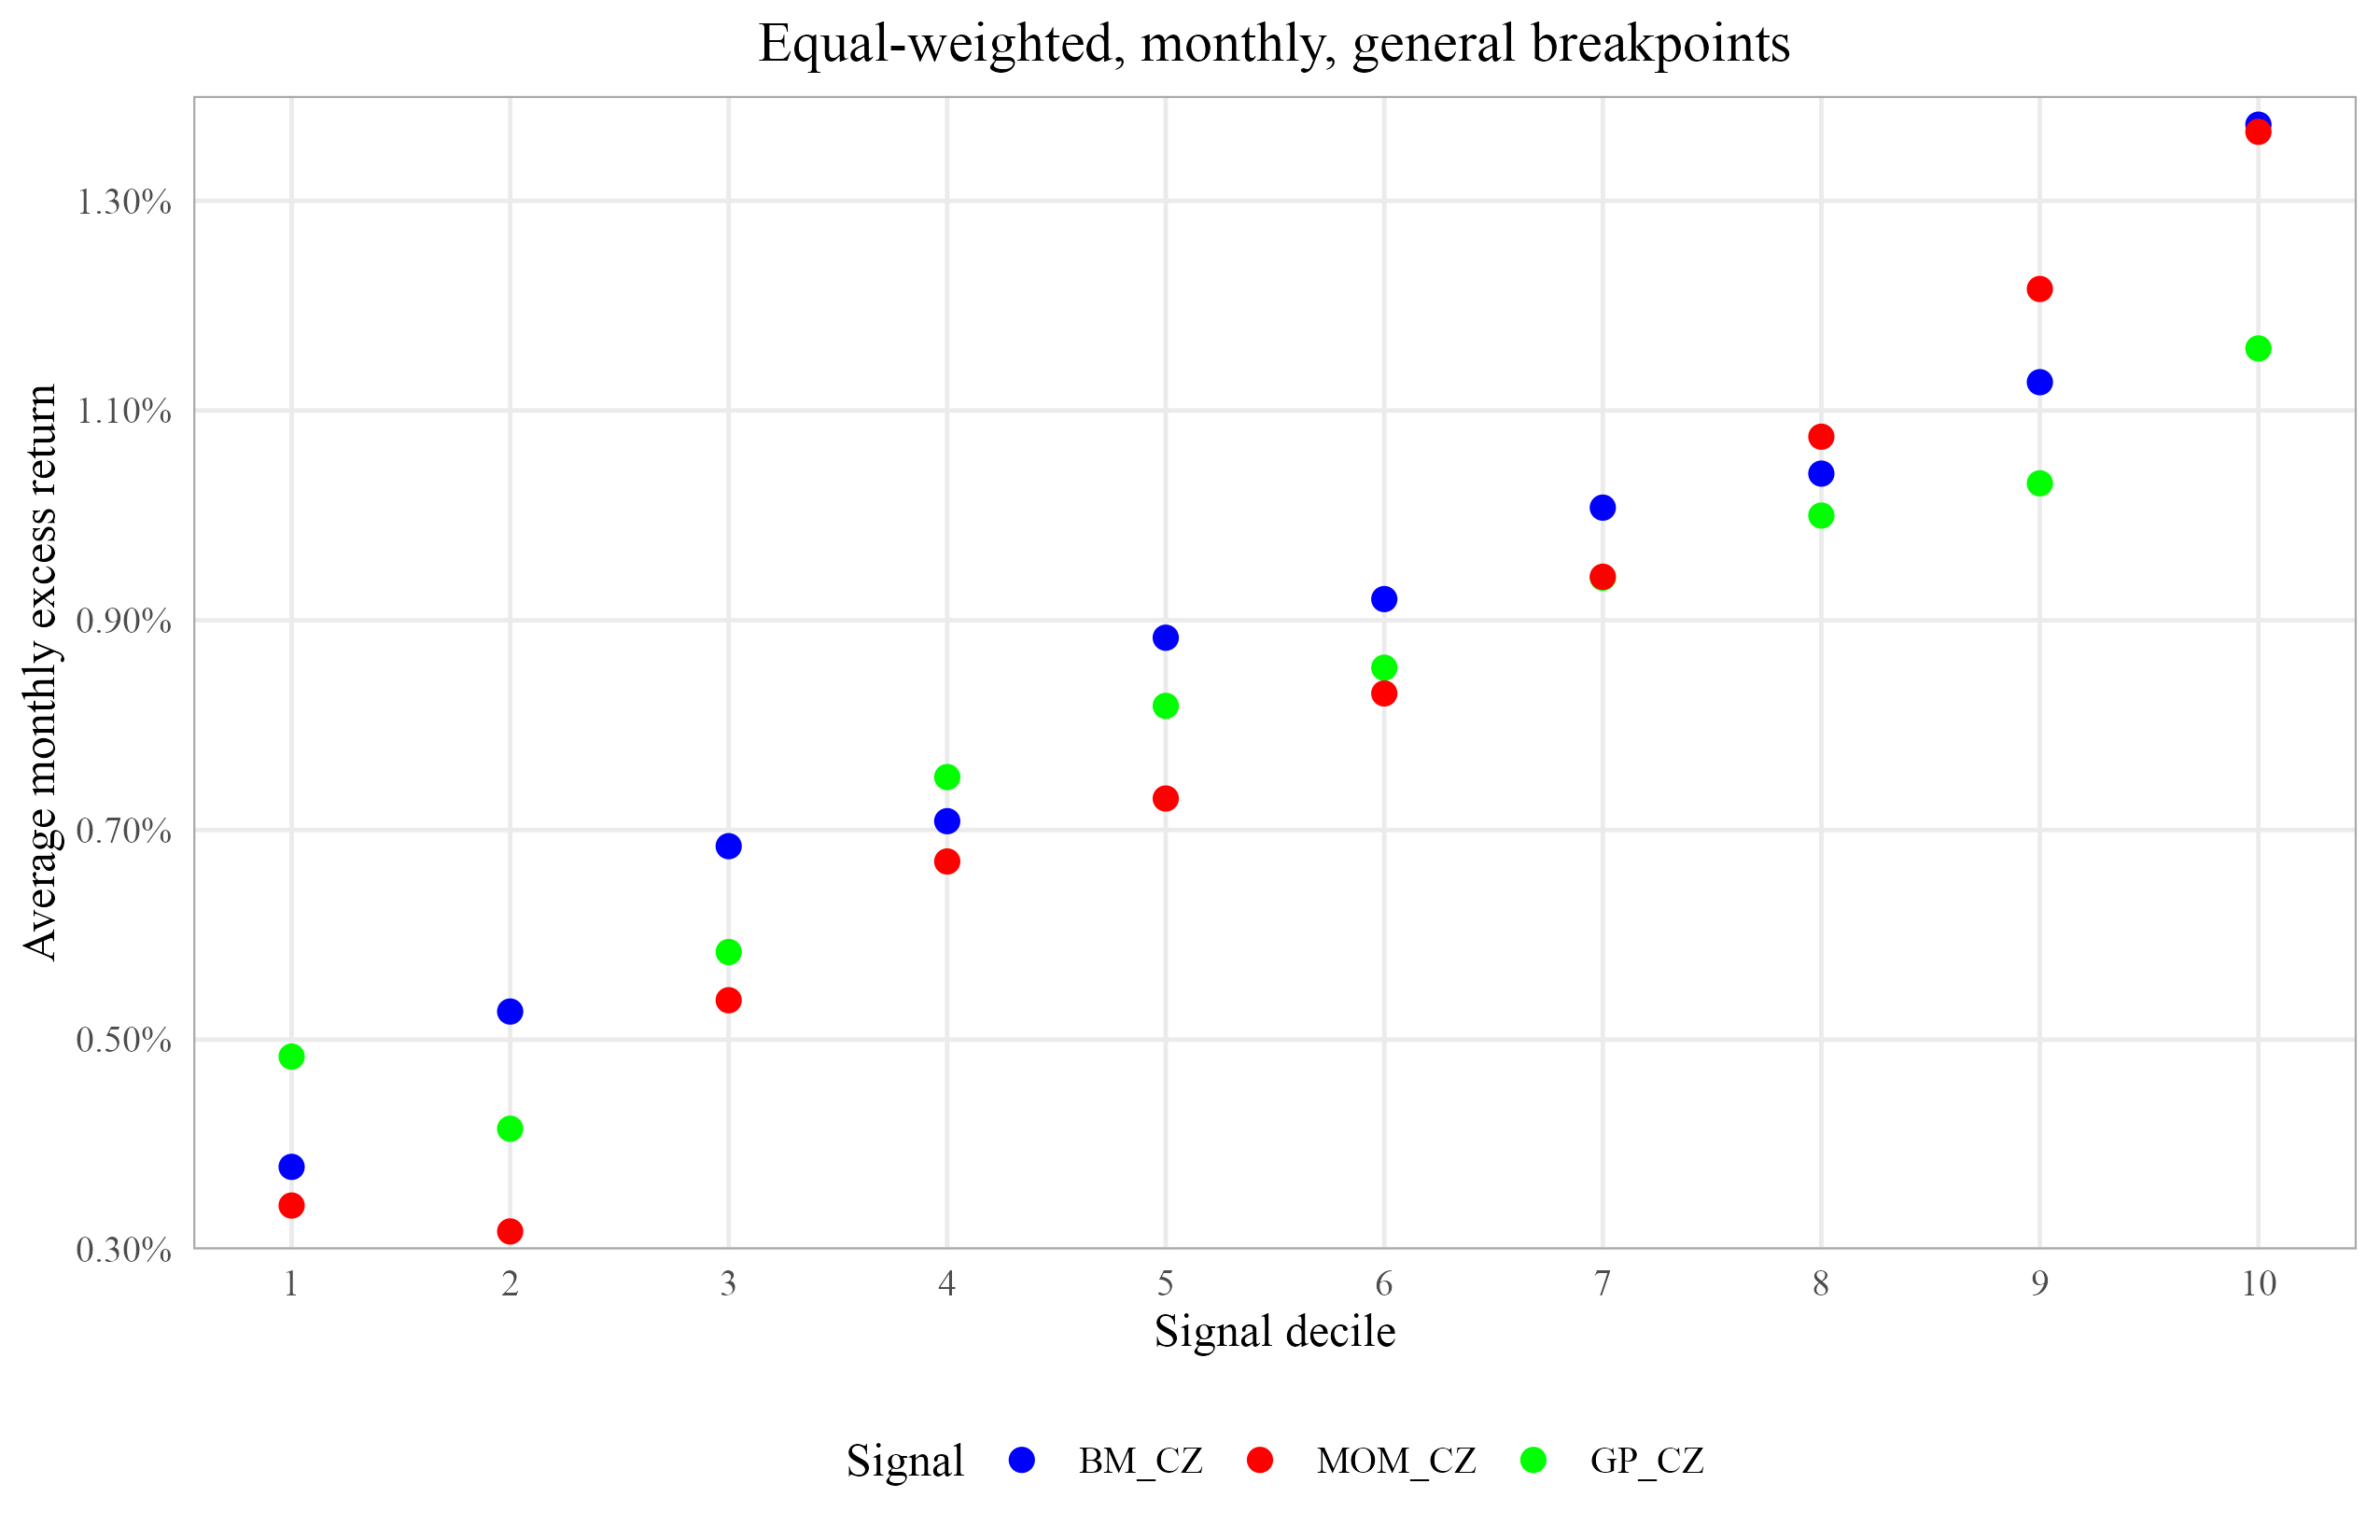
\includegraphics[width=0.70\textwidth]{figures/3c_v.png}
    \label{fig:q20}
\end{figure}

Across all scatterplots, higher decile portfolios have higher average excess returns than lower decile portfolios for each signal, which is consistent with their underlying principles. For instance, the book-to-market $BM\_CZ$ signal represents the value premium, positing that firms with high $BM\_CZ$ (value firms) tends to generate higher future returns than firms with low $BM\_CZ$ (growth firms). $MOM\_CZ$ captures the momemtum signal via returns from month t-12 to t-1 and suggests that recent winners (high $MOM\_CZ$) are likely to present higher future returns than recent losers (low $MOM\_CZ$). Finally, the profitability signal, $GP\_CZ$, suggests that firms with high gross profits/total assets tends to generate higher future returns than counterparts with low gross profits/ total assets. In addition, I also calculated the average HML excess returns of 15 HML portfolios for each pair of signal - portfolio construction method.  

\begin{table}[H]
  \centering
  \caption{Average excess HML portfolio returns \& t-statistic for each signal - portfolio construction pair}
  \label{tab:3c_hml}
  \begin{tabular}{lrrrrr}
    \hline
    Signal & Mean HML & Newey--West SE & $t$-statistic & Lag & $T$ \\
    \hline
    \multicolumn{6}{l}{\textit{Panel i: Value-weighted, annual, NYSE breakpoints}} \\
    BM\_CZ & 0.002972 & 0.002017 & 1.474 & 1 & 738 \\
    GP\_CZ & 0.003471 & 0.001630 & 2.129 & 8 & 738 \\
    MOM\_CZ & 0.005151 & 0.002268 & 2.271 & 6 & 738 \\
    \hline
    \multicolumn{6}{l}{\textit{Panel ii: Equal-weighted, annual, NYSE breakpoints}} \\
    BM\_CZ & 0.009895 & 0.001874 & 5.281 & 11 & 738 \\
    GP\_CZ & 0.005982 & 0.001695 & 3.529 & 11 & 738 \\
    MOM\_CZ & 0.000046 & 0.002085 & 0.022 & 5 & 738 \\
    \hline
    \multicolumn{6}{l}{\textit{Panel iii: Value-weighted, monthly, NYSE breakpoints}} \\
    BM\_CZ & 0.003219 & 0.002014 & 1.598 & 3 & 738 \\
    GP\_CZ & 0.003444 & 0.001686 & 2.042 & 10 & 738 \\
    MOM\_CZ & 0.012548 & 0.002717 & 4.619 & 1 & 738 \\
    \hline
    \multicolumn{6}{l}{\textit{Panel iv: Value-weighted, annual, general breakpoints}} \\
    BM\_CZ & 0.003438 & 0.002439 & 1.410 & 8 & 738 \\
    GP\_CZ & 0.004335 & 0.002092 & 2.072 & 7 & 738 \\
    MOM\_CZ & 0.007482 & 0.002910 & 2.571 & 4 & 738 \\
    \hline
    \multicolumn{6}{l}{\textit{Panel v: Equal-weighted, monthly, general breakpoints}} \\
    BM\_CZ & 0.009939 & 0.001909 & 5.206 & 10 & 738 \\
    GP\_CZ & 0.006754 & 0.002191 & 3.082 & 12 & 738 \\
    MOM\_CZ & 0.010240 & 0.003073 & 3.332 & 10 & 738 \\
    \hline
  \end{tabular}
\end{table}

Again, the mean HML excess returns in decimals are positive across all signals and sorting methods, reinforcing the idea that higher value, profitability, and momentum signals imply higher future returns. However, their magnitudes and statistical significance differ. Only $GP\_CZ$ is the most robust across 5 types of portfolios with average HML excess returns ranging from 0.30\% to 0.99\%. Meanwhile, $BM\_CZ$ is only statistically significant in equally weighted portfolios, suggesting that their predictability power is stronger among smaller firms. $MOM\_CZ$ is statistically insignificant with almost zero average HML excess returns in equally weighted, annually rebalanced portfolios with NYSE breakpoints. 

\subsection*{3 (d)} 
I used a common sample of 618 months from July 1973 to December 2024 by doing left join of $DUR$ from Goncalves (2021b), $GP\_CZ$ and $BM\_CZ$ from Chen \& Zimmermann (2022), $RF$ from Fama \& French's 3 Factor Model (1993) with the CRSP monthly $XRET\_ADJ$ constructed in part (a) on $PERMNO$ and $DUR\_YEAR$. In particular, $DUR\_YEAR$ denotes that $DUR$ is fixed for 12 calender months from June of year t to May of year t+1, which is consistent with the timing of $BM\_CZ$. For each signal $X$, within each month $\tau$, I sorted $N_{\tau}$ stocks in an ascending order and assigned its rank in the cross-sectional distribution of $X$ as $R_{j, \tau} = rank(X_{j, \tau})$. Then, I calculated its respective cross-sectional percentile rank as $Q_{j, \tau} = R_{j, \tau}/ N_\tau$ where $Q_{j, \tau} \in (0,1]$. I proceeded to estimate 7 monthly cross-sectional regressions using both OLS and WLS as follows: 
\[
\begin{aligned}
\text{(i)}\quad
xR_{j,\tau+1}
&=
a_{\tau+1}
+b^{BM}_{\tau+1} \cdot Q^{BM}_{j,\tau}
+e_{j,\tau+1},
\\[4pt]
\text{(ii)}\quad
xR_{j,\tau+1}
&=
a_{\tau+1}
+b^{GP}_{\tau+1} \cdot Q^{GP}_{j,\tau}
+e_{j,\tau+1},
\\[4pt]
\text{(iii)}\quad
xR_{j,\tau+1}
&=
a_{\tau+1}
+b^{Dur}_{\tau+1} \cdot Q^{Dur}_{j,\tau}
+e_{j,\tau+1},
\\[4pt]
\text{(iv)}\quad
xR_{j,\tau+1}
&=
a_{\tau+1}
+b^{BM}_{\tau+1} \cdot Q^{BM}_{j,\tau}
+b^{GP}_{\tau+1} \cdot Q^{GP}_{j,\tau}
+e_{j,\tau+1},
\\[4pt]
\text{(v)}\quad
xR_{j,\tau+1}
&=
a_{\tau+1}
+b^{Dur}_{\tau+1} \cdot Q^{Dur}_{j,\tau}
+b^{BM}_{\tau+1} \cdot Q^{BM}_{j,\tau}
+e_{j,\tau+1},
\\[4pt]
\text{(vi)}\quad
xR_{j,\tau+1}
&=
a_{\tau+1}
+b^{Dur}_{\tau+1} \cdot Q^{Dur}_{j,\tau}
+b^{GP}_{\tau+1} \cdot Q^{GP}_{j,\tau}
+e_{j,\tau+1},
\\[4pt]
\text{(vii)}\quad
xR_{j,\tau+1}
&=
a_{\tau+1}
+b^{Dur}_{\tau+1} \cdot Q^{Dur}_{j,\tau}
+b^{BM}_{\tau+1} \cdot Q^{BM}_{j,\tau}
+b^{GP}_{\tau+1} \cdot Q^{GP}_{j,\tau}
+e_{j,\tau+1}.
\end{aligned}
\]

For each regression specification and method, I retrieved the time series of the slope coefficients and obtained the Fama-Macbeth estimate $b_{FM}$ for each signal $X$ as follows:
\[
    \widehat b_{\tau+1}^{X} = b_{FM}^{X} + \eta_{\tau+1}^{X} 
\]

Then, I computed the Newey-West (1987, 1994) standard errors to account for autocorrelation in $e_{j,\tau+1}$ and obtained the following results: 

\begin{table}[H]
  \centering
  \caption{Fama--MacBeth regressions of monthly stock excess returns}
  \label{tab:3d}
  \resizebox{\textwidth}{!}{%
  \begin{tabular}{lrrrrrrr}
    \toprule
    & (i) & (ii) & (iii) & (iv) & (v) & (vi) & (vii) \\
    \midrule
    \multicolumn{8}{l}{\textit{Panel A: OLS}} \\
    Intercept & $0.0046$ & $0.0040$ & $0.0161^{***}$ & $-0.0009$ & $0.0143^{***}$ & $0.0143^{***}$ & $0.0096^{***}$ \\
    & $(1.50)$ & $(1.20)$ & $(6.85)$ & $(-0.27)$ & $(5.79)$ & $(5.10)$ & $(3.35)$ \\
    $b_{BM}$ & $0.0097^{***}$ &  &  & $0.0109^{***}$ & $0.0022$ &  & $0.0044$ \\
    & $(4.22)$ &  &  & $(4.65)$ & $(0.76)$ &  & $(1.34)$ \\
    $b_{GP}$ &  & $0.0093^{***}$ &  & $0.0095^{***}$ &  & $0.0026$ & $0.0042^{**}$ \\
    &  & $(4.71)$ &  & $(4.90)$ &  & $(1.48)$ & $(2.24)$ \\
    $b_{Dur}$ &  &  & $-0.0122^{***}$ &  & $-0.0110^{***}$ & $-0.0114^{***}$ & $-0.0085^{***}$ \\
    &  &  & $(-6.45)$ &  & $(-4.37)$ & $(-5.66)$ & $(-3.01)$ \\
    Average $R^2$ & 0.006 & 0.005 & 0.007 & 0.010 & 0.012 & 0.010 & 0.014 \\
    Average $N$ & 3130 & 3357 & 2365 & 3024 & 2344 & 2311 & 2307 \\
    \midrule
    \multicolumn{8}{l}{\textit{Panel B: WLS}} \\
    Intercept & $0.0061^{***}$ & $0.0041^{*}$ & $0.0132^{***}$ & $0.0011$ & $0.0132^{***}$ & $0.0076^{*}$ & $0.0041$ \\
    & $(2.68)$ & $(1.71)$ & $(6.78)$ & $(0.38)$ & $(3.90)$ & $(1.94)$ & $(1.05)$ \\
    $b_{BM}$ & $0.0027$ &  &  & $0.0061^{**}$ & $-0.0021$ &  & $0.0031$ \\
    & $(0.91)$ &  &  & $(2.05)$ & $(-0.53)$ &  & $(1.07)$ \\
    $b_{GP}$ &  & $0.0044^{**}$ &  & $0.0064^{***}$ &  & $0.0058^{*}$ & $0.0067^{**}$ \\
    &  & $(1.98)$ &  & $(3.11)$ &  & $(1.74)$ & $(2.38)$ \\
    $b_{Dur}$ &  &  & $-0.0089^{***}$ &  & $-0.0080^{**}$ & $-0.0052$ & $-0.0023$ \\
    &  &  & $(-3.09)$ &  & $(-2.25)$ & $(-1.26)$ & $(-0.62)$ \\
    Average $R^2$ & 0.023 & 0.019 & 0.017 & 0.037 & 0.039 & 0.043 & 0.051 \\
    Average $N$ & 3129 & 3355 & 2364 & 3023 & 2342 & 2310 & 2306 \\
    \bottomrule
  \end{tabular}%
  }
  \begin{minipage}{\textwidth}
  \footnotesize \textit{Notes:} Each column reports time-series averages of monthly cross-sectional coefficient estimates. Newey--West $t$-statistics are in parentheses. WLS uses month-$\tau$ market-equity weights normalized within each valid monthly regression sample. $^{***}$, $^{**}$, and $^{*}$ denote significance at the 1\%, 5\%, and 10\% levels, respectively.
  \end{minipage}
\end{table}

Looking at the results of OLS regressions, $\widehat{b}_{DUR}$ is negative and statistically significant across all regression specifications, which is consistent with the existence of the short duration premium (Goncalves, 2021b). In particular, firms with high ranks in $DUR$ (long duration stocks) tend to generate lower future returns than short duration counterparts. Controlling for both $GP\_CZ$ and $BM\_CZ$, $DUR$'s magnitude remained meaningful at -0.85\%, far outweighing the other two signals. While $BM\_CZ$ and $GP\_CZ$ were statistically signifincant in their standalone and joint regressions, these premia vanished after controlling for $DUR$. When all 3 signals were included in an OLS regression, only $DUR$ was statistically significant at 1\% level, while $GP\_CZ$ was statistically significant at 5\% level and $BM\_CZ$ disappeared. Examining the regression results of $ME$-weighted WLS, the magnitude and statistical significance of $DUR$ declined, suggesting that the short duration premium is not as strong in firms with high market capitalization. However, this difference could be merely due to a construction issue as I did not exclude microcaps nor winsorize returns as done by Goncalves (2021b). 

\subsection*{3 (e)}
I upheld the same merging techniques, timing decisions, and duplicate protocols in the previous parts. Similar to part (c), I constructed signal-specific decile portfolios using NYSE breakpoints for the entire valid stock universe. As a result, at time $\tau$, a stock has 3 decile assigments, namely $D_{j,\tau}^{X}$, and belongs to 1 of 10 decile portfolios, namely $P_{i, \tau}^{X}$ for $i = 1,\ldots,10$ and $X \in \{GP\_CZ, BM\_CZ, DUR\}$. For each decile portfolio $P$ at time $\tau$, I calculated excess returns using equal-weight and $ME$-weight methods and the average signal decile values as $Dec_{P, \tau}^{X} = \frac{1}{N_{P, \tau}^{X}} \cdot \sum_{j \in P} D_{j,\tau}^{X}$. Then, I proceeded to run the following multivaritate panel regressions of excess returns on average portfolio deciles: 
\[
\begin{aligned}
\text{(i)}\quad
xR_{P,\tau+1}
&=
a_{\tau+1}
+b^{BM}_{\tau+1} \cdot Dec^{BM}_{P,\tau}
+e_{P,\tau+1},
\\[4pt]
\text{(ii)}\quad
xR_{P,\tau+1}
&=
a_{\tau+1}
+b^{GP}_{\tau+1} \cdot Dec^{GP}_{P,\tau}
+e_{P,\tau+1},
\\[4pt]
\text{(iii)}\quad
xR_{P,\tau+1}
&=
a_{\tau+1}
+b^{Dur}_{\tau+1} \cdot Dec^{Dur}_{P,\tau}
+e_{P,\tau+1},
\\[4pt]
\text{(iv)}\quad
xR_{P,\tau+1}
&=
a_{\tau+1}
+b^{BM}_{\tau+1} \cdot Dec^{BM}_{P,\tau}
+b^{GP}_{\tau+1} \cdot Dec^{GP}_{P,\tau}
+e_{P,\tau+1},
\\[4pt]
\text{(v)}\quad
xR_{P,\tau+1}
&=
a_{\tau+1}
+b^{Dur}_{\tau+1} \cdot Dec^{Dur}_{P,\tau}
+b^{BM}_{\tau+1} \cdot Dec^{BM}_{P,\tau}
+e_{P,\tau+1},
\\[4pt]
\text{(vi)}\quad
xR_{P,\tau+1}
&=
a_{\tau+1}
+b^{Dur}_{\tau+1} \cdot Dec^{Dur}_{P,\tau}
+b^{GP}_{\tau+1} \cdot Dec^{GP}_{P,\tau}
+e_{P,\tau+1},
\\[4pt]
\text{(vii)}\quad
xR_{P,\tau+1}
&=
a_{\tau+1}
+b^{Dur}_{\tau+1} \cdot Dec^{Dur}_{P,\tau}
+b^{BM}_{\tau+1} \cdot Dec^{BM}_{P,\tau}
+b^{GP}_{\tau+1} \cdot Dec^{GP}_{P,\tau}
+e_{P,\tau+1}.
\end{aligned}
\]

\begin{table}[H]
  \centering
  \caption{Pooled regressions of portfolio excess returns}
  \label{tab:3e}
  \resizebox{\textwidth}{!}{%
  \begin{tabular}{lrrrrrrr}
    \toprule
    & (i) & (ii) & (iii) & (iv) & (v) & (vi) & (vii) \\
    \midrule
    \multicolumn{8}{l}{\textit{Panel A: Value-weighted portfolios}} \\
    Intercept & $0.0058^{***}$ & $0.0049^{**}$ & $0.0117^{***}$ & $0.0023$ & $0.0094^{***}$ & $0.0130^{***}$ & $0.0113^{*}$ \\
    & $(2.82)$ & $(2.11)$ & $(5.94)$ & $(0.93)$ & $(3.24)$ & $(4.12)$ & $(1.87)$ \\
    $b_{BM}$ & $0.0003$ &  &  & $0.0005^{*}$ & $0.0003$ &  & $0.0001$ \\
    & $(1.43)$ &  &  & $(1.90)$ & $(0.82)$ &  & $(0.26)$ \\
    $b_{GP}$ &  & $0.0003$ &  & $0.0004^{**}$ &  & $-0.0002$ & $-0.0001$ \\
    &  & $(1.54)$ &  & $(2.23)$ &  & $(-0.81)$ & $(-0.29)$ \\
    $b_{Dur}$ &  &  & $-0.0006^{***}$ &  & $-0.0005^{*}$ & $-0.0008^{***}$ & $-0.0007$ \\
    &  &  & $(-3.18)$ &  & $(-1.86)$ & $(-3.13)$ & $(-1.64)$ \\
    $R^2$ & 0.000 & 0.000 & 0.001 & 0.000 & 0.001 & 0.001 & 0.001 \\
    Observations & 6180 & 6180 & 6180 & 12360 & 12360 & 12360 & 18540 \\
    \midrule
    \multicolumn{8}{l}{\textit{Panel B: Equal-weighted portfolios}} \\
    Intercept & $0.0047$ & $0.0051$ & $0.0155^{***}$ & $-0.0038$ & $0.0132^{***}$ & $0.0155^{***}$ & $0.0078$ \\
    & $(1.63)$ & $(1.62)$ & $(6.29)$ & $(-1.03)$ & $(4.01)$ & $(4.54)$ & $(1.20)$ \\
    $b_{BM}$ & $0.0009^{***}$ &  &  & $0.0012^{***}$ & $0.0003$ &  & $0.0006$ \\
    & $(4.54)$ &  &  & $(5.34)$ & $(1.06)$ &  & $(1.37)$ \\
    $b_{GP}$ &  & $0.0007^{***}$ &  & $0.0011^{***}$ &  & $0.0001$ & $0.0005$ \\
    &  & $(5.09)$ &  & $(6.07)$ &  & $(0.41)$ & $(1.58)$ \\
    $b_{Dur}$ &  &  & $-0.0010^{***}$ &  & $-0.0010^{***}$ & $-0.0012^{***}$ & $-0.0008^{*}$ \\
    &  &  & $(-6.45)$ &  & $(-3.40)$ & $(-5.35)$ & $(-1.90)$ \\
    $R^2$ & 0.002 & 0.001 & 0.002 & 0.002 & 0.002 & 0.002 & 0.002 \\
    Observations & 6180 & 6180 & 6180 & 12360 & 12360 & 12360 & 18540 \\
    \bottomrule
  \end{tabular}%
  }
  \begin{minipage}{\textwidth}
  \footnotesize \textit{Notes:} The sample is July 1973--December 2024. Driscoll--Kraay $t$-statistics are in parentheses and use \texttt{plm::vcovSCC} with \texttt{type = HC0}, \texttt{inner = cluster}, Bartlett weights, four lags from $\lfloor T^{1/4}\rfloor$, and no finite-sample adjustment. $^{***}$, $^{**}$, and $^{*}$ denote significance at the 1\%, 5\%, and 10\% levels, respectively.
  \end{minipage}
\end{table}

The initial result of the pooled OLS regressions on porfolios deciles is in line with the Fama-MacBeth regressions on firm-level percentile ranks. Given a negative $\hat{b}_{Dur}$, longer duration stocks tend to generate lower excess return in the following month compared to shorter duration stocks, pointing to the short duration premium. However, its effect is only significant at 10\% level for equal-weighted portfolios and is insignificant for value-weighted portfolios. Looking into its interaction with $BM\_CZ$ and $GP\_CZ$, controlling for $DUR$ made the value and profitability premia vanish in their joint regressions for both types of portfolios. In the joint regressions of 3 signals, only equal-weighted portfolios yielded a statistically significant $\hat{b}_{DUR}$, thus suggesting that the short duration premium effect may not be strong for large-cap firms. 


\section*{Question 4}
\subsection*{4 (a)} 
I selected Fama-Bliss discount bonds with maturities of 1-5 years by first, filtering those with KYTREASNOX from 2000047 to 2000051 and, second, verifying the mapping with 5 unique combinations of KYTREASNOX and TTERMLBL. Obtaining the decimal yield by dividing TMYTM by 100, I calculated the following: 
\begin{enumerate}
    \item For $H = 1,\ldots,5$, log yield $y_t^{H} = log(1+Y_t^{H})$
    \item For $H = 2,\ldots,5$, log forward rate $f_t^{H} = H \cdot y_t^{H} - (H-1) \cdot y_t^{H-1}$ with $f_t^{1} = y_t^{1}$
    \item For $H = 2,\ldots,5$, log annual return $r_t^{H} = H \cdot y_{t-1}^{H} - (H-1) \cdot y_t^{H-1}$, with $r_t^{1} = y_{t-1}^{1}$, where $y_{t-1}^{1}$ is the 12-month lag of $y_t^{1}$.
\end{enumerate}

By subtracting $y_t^{1}, f_t^{1}$ and $r_t^{1}$ from these variables and taking their averages across H = 2,...,5, I obtained the following table: 

\begin{table}[H]
  \centering
  \caption{Average excess bond yields, forward rates, and annual returns}
  \label{tab:q4a}
  \begin{tabular}{crrr}
    \toprule
    $H$ & $\overline{xy}_{t}^{(H)}$ & $\overline{xf}_{t}^{(H)}$ & $\overline{xr}_{t}^{(H)}$ \\
    \midrule
    2 & 0.001686 & 0.003372 & 0.003154 \\
    3 & 0.003278 & 0.006461 & 0.006069 \\
    4 & 0.004660 & 0.008805 & 0.008198 \\
    5 & 0.005639 & 0.009557 & 0.008719 \\
    \bottomrule
  \end{tabular}
\end{table}

\subsection*{4 (b)} 
For $H = 2,\ldots,5$, I estimated the OLS regression of long-term excess returns on excess log yield as follows: 
\[
    (1/H) \cdot xr_{t \to t+H}^{H} = a^{H} + b^{H} \cdot xy_{t}^{H} + e_{t}^{H}
\]

where the hold-to-maturity excess return is $xr_{t \to t+H}^{H} = \sum_{h=1}^{H} xr_{t+h}^{(H-h+1)}$. Using a common set of 811-month sample from June 1952 to December 2019 and the Hansen-Hodrick standard errors with $L = Overlap = 12H-1$, I derived the estimated $b^{H}$, t-stat, and $R^2$ for each maturity as follows: 
\begin{table}[H]
  \centering
  \caption{Predictive regressions for hold-to-maturity excess bond returns}
  \label{tab:q4b}
  \begin{tabular}{crrr}
    \toprule
    $H$ & $\hat{b}^{(H)}$ & Hansen--Hodrick $t$-stat & $R^2$ \\
    \midrule
    2 & 0.6931 & 3.4373 & 0.0809 \\
    3 & 0.5201 & 2.9989 & 0.0543 \\
    4 & 0.3935 & 2.2761 & 0.0379 \\
    5 & 0.3140 & 2.0716 & 0.0281 \\
    \bottomrule
  \end{tabular}
\end{table} 

As observed in the table, $\hat{b}^{(H)}$ remains positive across all maturities, suggesting that a higher term spread predicts higher long-horizon hold-to-maturity excess return. As H increases, t-stat and $R^{2}$ decreases, which is consistent with the notion of time-varying bond risk premia.  

\subsection*{4 (c)} 
For $H = 2,\ldots,5$, I estimated the OLS regression of 1-year excess returns on log forward spreads as follows: 
\[
    xr_{t+1}^{H} = a^{H} + b^{H} \cdot xf_{t}^{H} + e_{t}^{H}
\]
Using a common set of 811-month sample from June 1952 to December 2019 and the Newey-West standard errors with a Barlett kernel and chosen lags of 20,20,20,19 for H = 2,3,4,5 respectively, I estimated the $b^{H}$, t-stat, and $R^{2}$ as follows: 
\begin{table}[H]
  \centering
  \caption{Predictive regressions of 1-year excess bond returns on log forward spreads}
  \label{tab:q4c}
  \begin{tabular}{crrr}
    \toprule
    $H$ & $\hat{b}^{(H)}$ & Newey--West $t$-stat & $R^2$ \\
    \midrule
    2 & 0.6931 & 3.0524 & 0.0809 \\
    3 & 0.9028 & 3.0669 & 0.0889 \\
    4 & 1.1476 & 3.4600 & 0.1148 \\
    5 & 0.9715 & 2.7420 & 0.0685 \\
    \bottomrule
  \end{tabular}
\end{table}

Similar to part (b), a steeper forward spread predicts higher 1-year excess bond returns across all maturities with the highest predictability in H = 4 years. In addition, I also verified that $\hat{b}^{(2)}$ in Equation (4.2) is equal to that in Equation (4.3), following the steps in Footnote 15. 

\subsection*{4 (d)} 
Following Cochrane and Piazzesi (2005), I regressed the average 1-year excess bond returns across maturities on a linear combination of forward rates for $H = 1,\ldots,5$, using 859 observations from June 1952 to December 2023 as follows: 
\[
    \frac{1}{4} \cdot \sum_{H=2}^{5} xr_{t+1}^{H} = \theta_{0} + \sum_{H=1}^{5} \theta_{h} \cdot f_{t}^{H} + u_t
\]

Then, replicating the construction in the paper, I used the $\hat{\theta}_{h}$ to estimate the common return-forecasting factor in decimals, defined as:
\[
    cp_{t} = \sum_{H=1}^{5} \hat{\theta}_{h} \cdot f_{t}^{H}
\]

\begin{figure}[H]
    \centering
    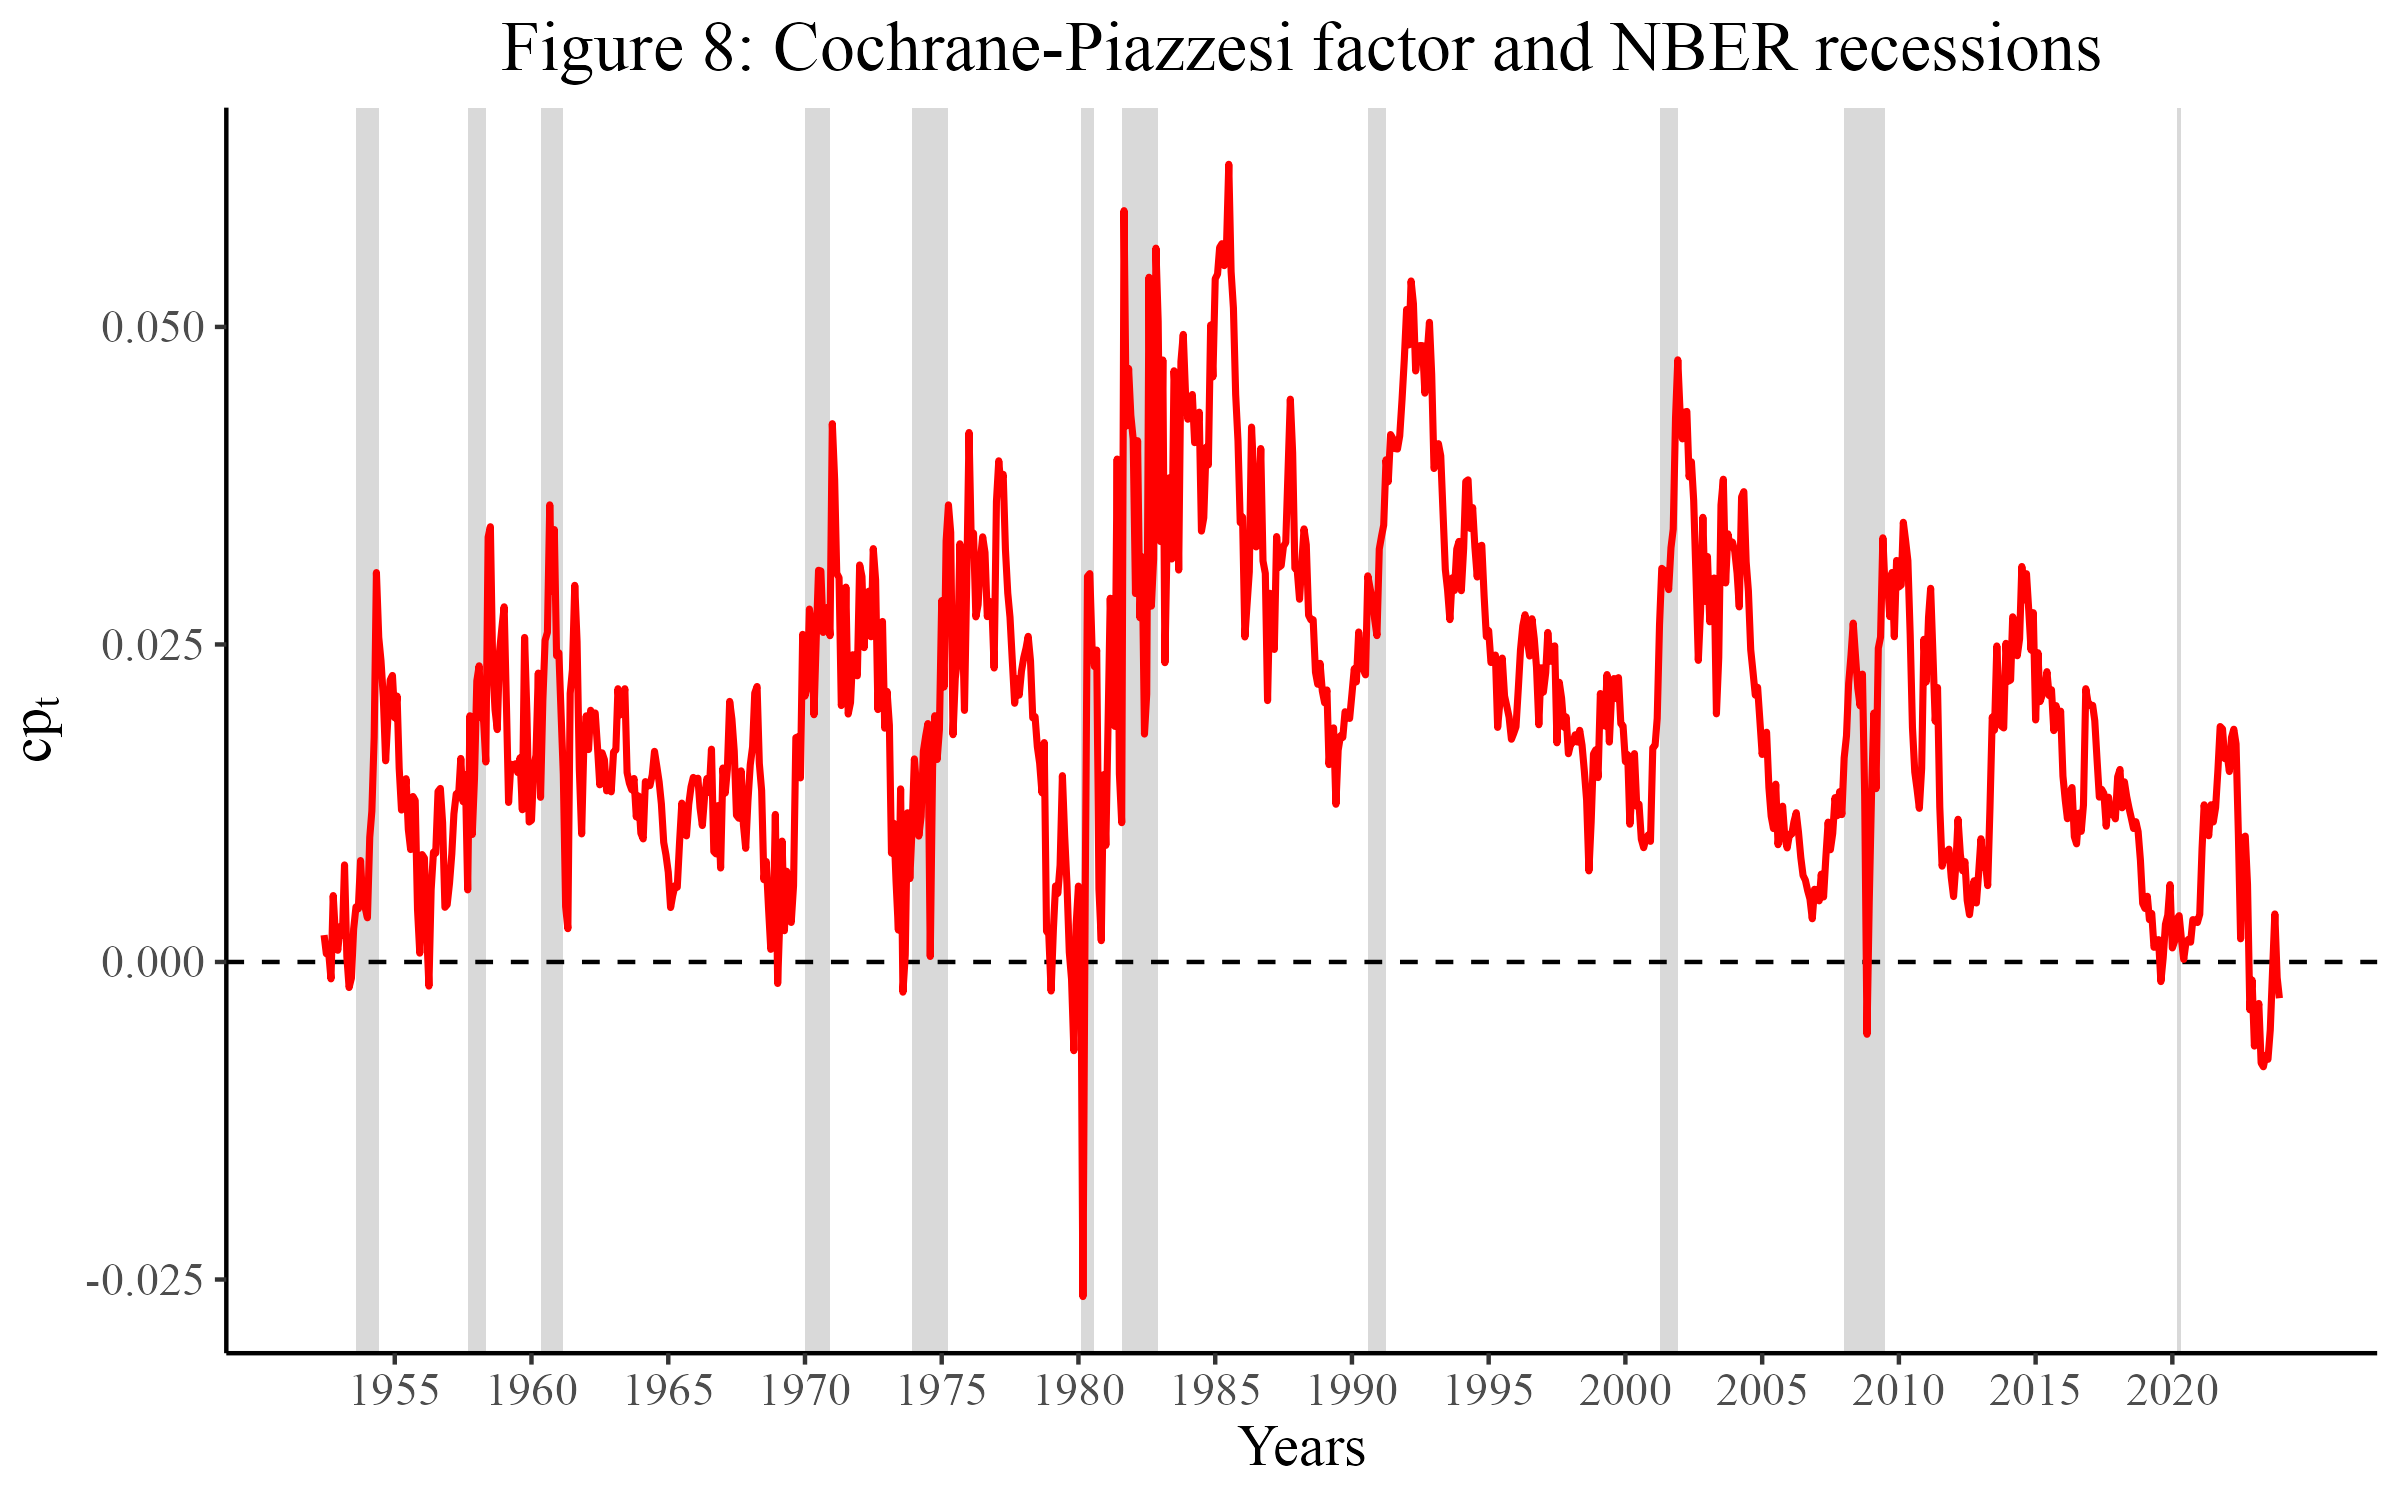
\includegraphics[width=0.8\textwidth]{figures/4d.png}
    \label{fig:q8}
\end{figure}

Figure 8 presented the time series of the common return-forecasting factor agaisnt the NBER recessions in grey. It is clear that $cp_{t}$ is countercyclical as it tends to be high when there is a recession, suggesting that investors demand higher excess returns during economic downturns. It is also worth noting that $cp_t$ also becomes negative, especially during highly inflationtionary periods in 1980 and 2023. This could be due to the tent-shaped pattern of the estimated $\hat{\theta}_{H}$ coefficients as demonstrated by Cochrane \& Piazzesi. Given that the coefficients are negative on the shorter term maturities of forward rates, elevated short-term rates relative to medium and long-term rates put downward pressure on the resulting $cp_t$, leading to negative $cp_t$ during those times. I attempted to verify the tent-shaped pattern of the forward rate coefficients, using data from 1952 to 2023 and retrieved a relatively similar observation. 

\begin{figure}[H]
    \centering
    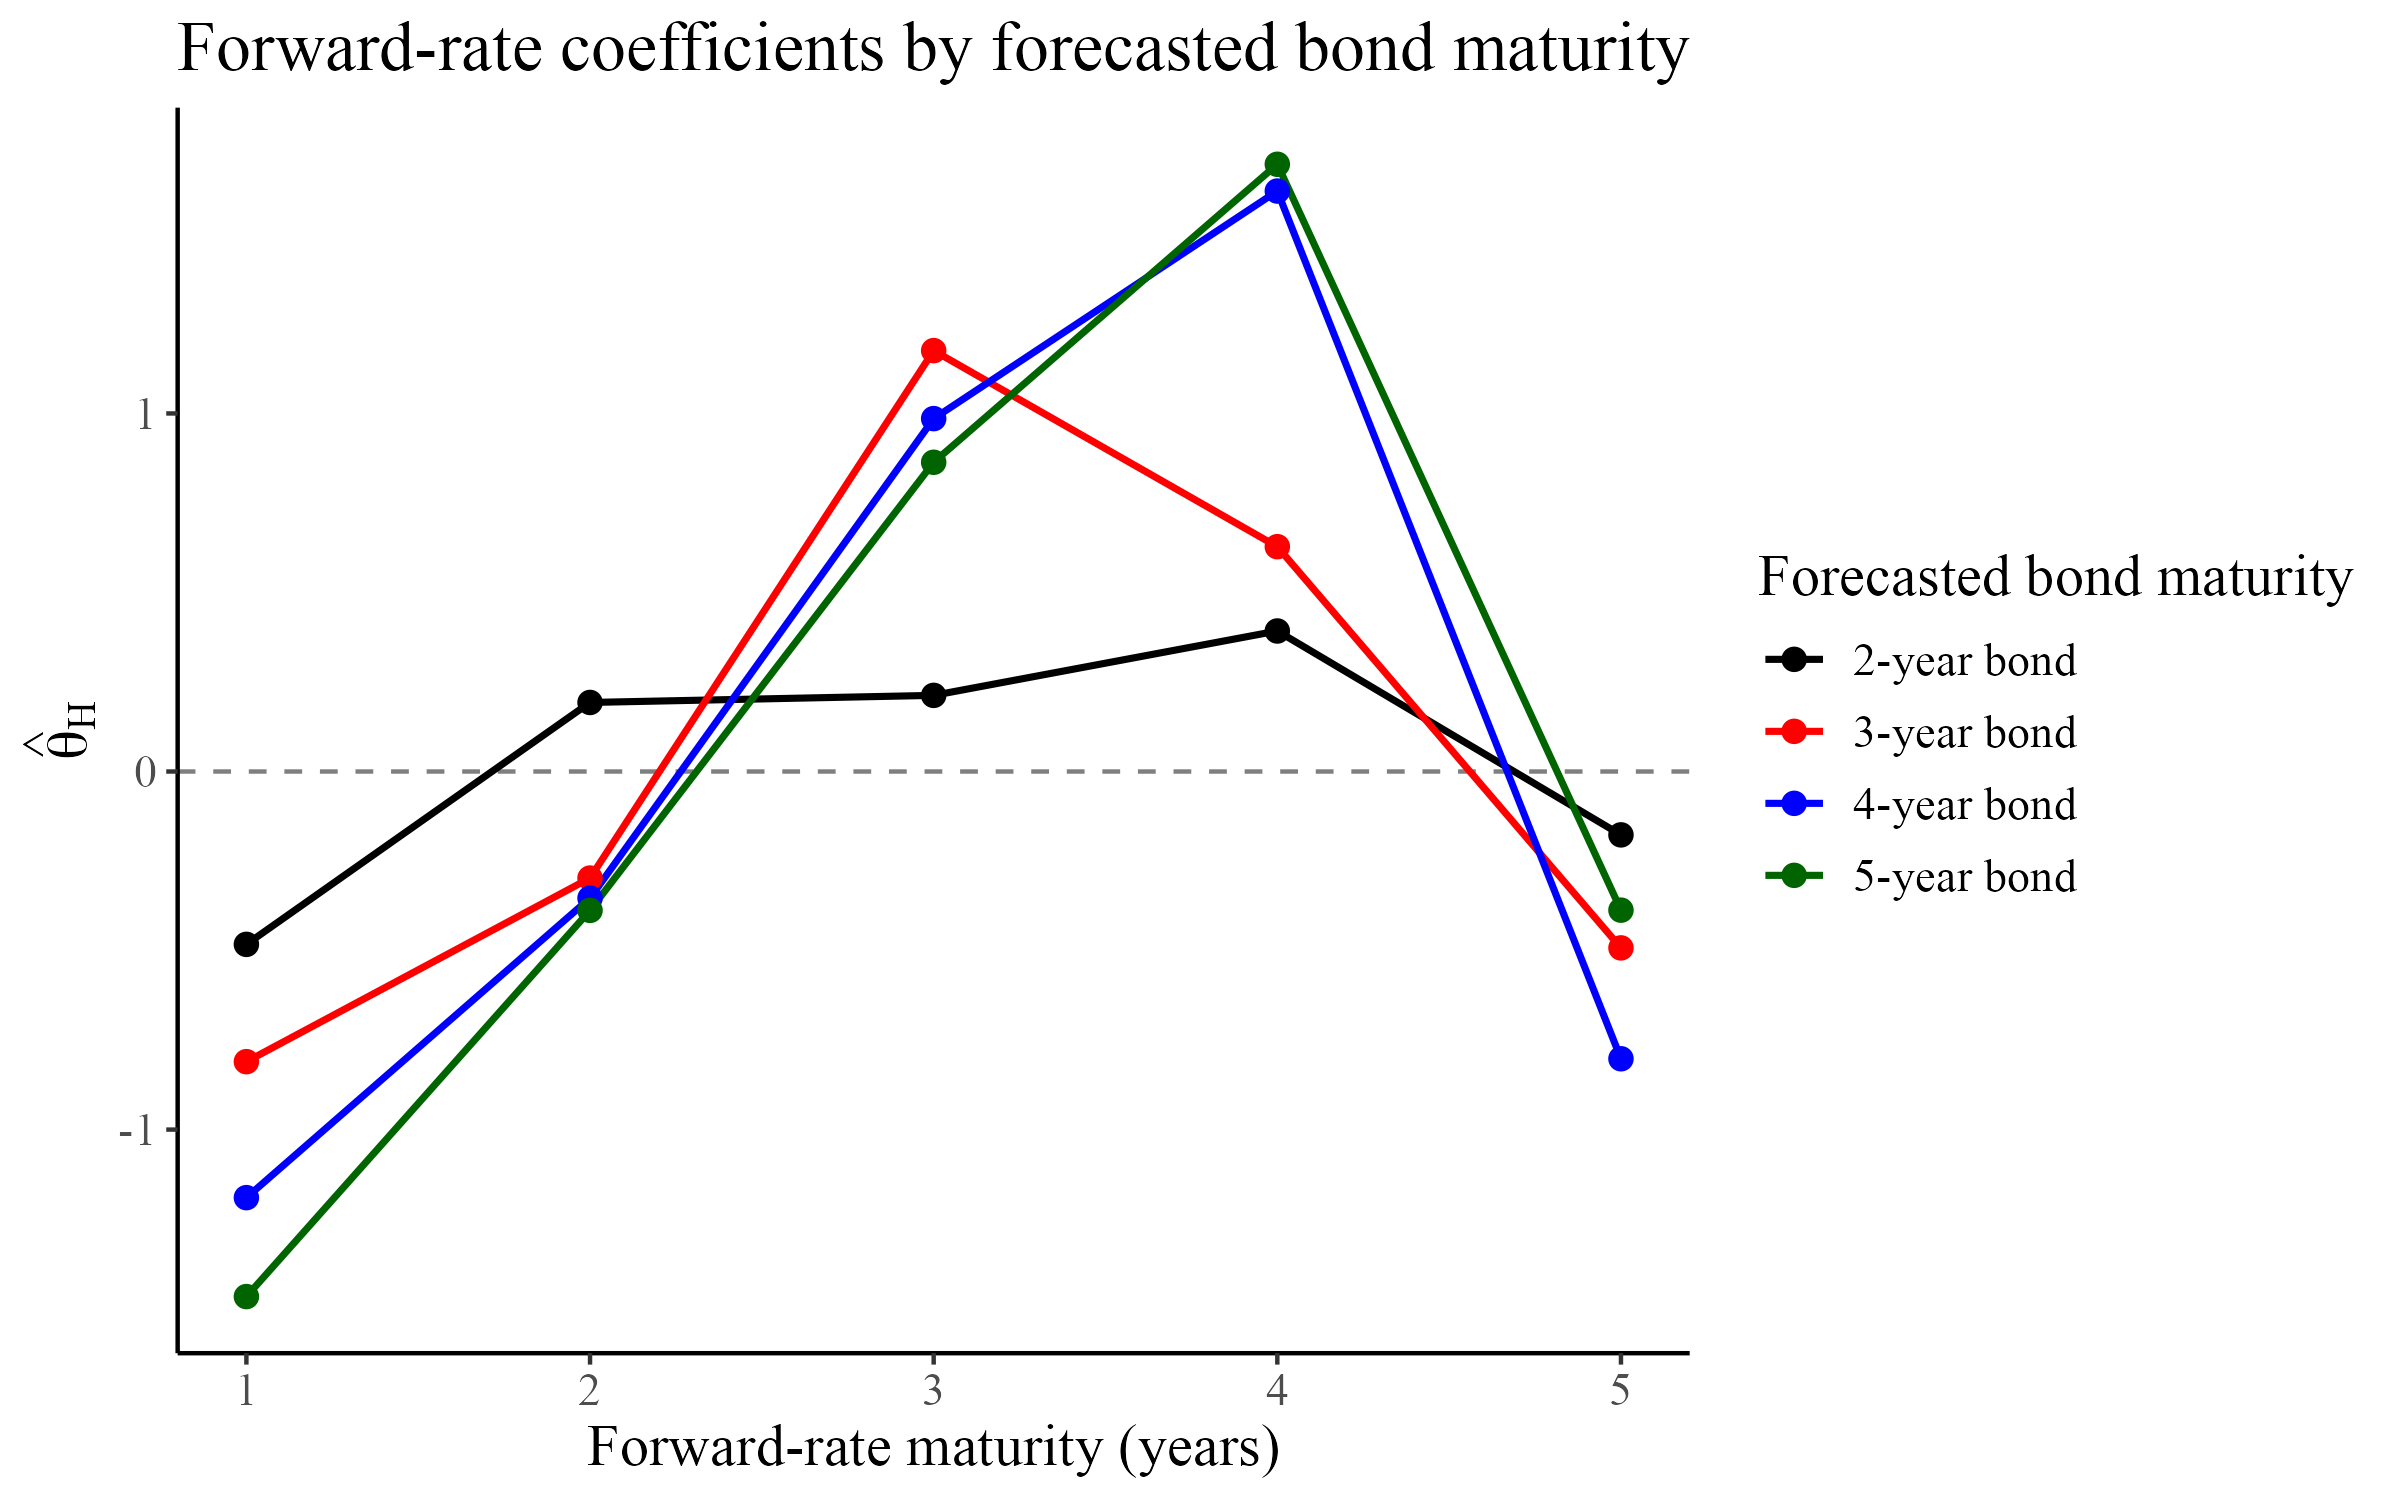
\includegraphics[width=0.75\textwidth]{figures/4d_2.png}
    \label{fig:q9}
\end{figure}

\subsection*{4 (e)} 
For $H = 2,\ldots,5$, I ran the OLS regression of 1-year excess returns on the Cochrane-Piazzesi factor as follows: 
\[
    xr_{t+1}^{H} = a^{H} + b^{H} \cdot cp_{t} + e_{t}^{H}
\]
Using a set of 859 observations from June 1952 to December 2023 and the Newey-West standard error with an automatically chosen lag of 21, I estimated $b_{H}$, t-statistics, and $R^{2}$ as follows:

\begin{table}[H]
  \centering
  \caption{Predictive regressions of 1-year excess bond returns on the Cochrane--Piazzesi factor}
  \label{tab:q4e}
  \begin{tabular}{crrr}
    \toprule
    $H$ & $\hat{b}^{(H)}$ & Newey--West $t$-stat & $R^2$ \\
    \midrule
    2 & 0.4418 & 4.1257 & 0.1367 \\
    3 & 0.8274 & 4.1243 & 0.1438 \\
    4 & 1.2517 & 4.3896 & 0.1705 \\
    5 & 1.4791 & 4.1986 & 0.1552 \\
    \bottomrule
  \end{tabular}
\end{table}

In comparison to the individual regressions of excess returns on log yield spreads and log forward spreads in part (b) and part (c), $cp_t$ significantly improves the predictability of excess returns, with t-stat and $R^{2}$ consistently above 1.96 and 12 \% across all maturities. Most importantly, $cp_t$ seems to carry additional information that helps it better predict 1-year excess bond returns with higher maturities. 

\end{document}
